%%%%%%%%%%%%%%%%%%%%%%%%%%%
%                         %
%       2016.11.16.       %
%      Szakdolgozat       %
%    Tamás     LATEX      %
%%%%%%%%%%%%%%%%%%%%%%%%%%%
\documentclass[oneside,titlepage,12pt,a4paper]{report}
%\documentclass[12pt]{report}
\usepackage[centertags]{amsmath}
\usepackage{amsfonts}
\usepackage{amsthm}
\usepackage{newlfont}
%\usepackage[ansinew]{inputenc}
\usepackage[magyar]{babel}	
\usepackage[utf8]{inputenc}		
\usepackage{t1enc}				
\usepackage{graphicx}
\usepackage{color}
%\usepackage[colorlinks]{hyperref}
%\usepackage[active,new,noold,marker]{xrcs}
\usepackage{euler}
\usepackage{amssymb,latexsym}
\usepackage{amsmath}
\usepackage{graphics}
\usepackage{algorithm} 
\usepackage{algpseudocode} %ezzel összeakadhat \usepackage{algorithmic} 
%\usepackage{algorithmic} 
\usepackage{rotating}
\usepackage{bigstrut}
\usepackage{subfigure}
\usepackage{appendix}
\usepackage{setspace}
\usepackage{adjustbox}


\newtheorem{theorem}{Theorem}
\newtheorem{corollary}{Corollary}
\newtheorem{lemma}{Lemma}
\newtheorem{proposition}{Proposition}
\newtheorem{definition}{Definition}
\newtheorem{notation}{Notation}

\textwidth=6.truein \textheight=9.truein \hoffset=-.5truein
\voffset=-.8truein

\frenchspacing				
\setlength{\parskip}{\smallskipamount}	
\renewcommand{\appendixtocname}{Függelék}
\renewcommand{\appendixpagename}{Függelék}
\DeclareMathOperator{\grad}{grad}
\DeclareMathOperator{\sgn}{sign}
\DeclareMathOperator{\PRD}{PRD}
\DeclareMathOperator{\CR}{CR}
\newcommand{\conj}[1]{\overline{#1}}

\begin{document}
\begin{titlepage}
	\parbox[t]{5.5cm}{\vspace{1cm}}
\begin{center}
	\large
	\textsc{Eötvös Loránd Tudományegyetem \linebreak Informatikai Kar} \\[2cm]
\end{center}

\begin{center}
	% Title
	\LARGE EKG jelek feldolgozása Hermite-függvények segítségével\\[0.55cm]
	\large BSc Szakdolgozat \\[1.9cm]
\end{center}

\begin{center}
	\parbox[t]{25mm}{Készítette:}
	\parbox[t]{5.5cm}
		{Dózsa Tamás\\
		ELTE IK\\
		Programtervező informatikus \\
		BSc
		}
	\\[0.9cm]
	
  \parbox[t]{25mm}{Témavezető:}
	\parbox[t]{5.5cm}{
		Dr. Kovács Péter\\
		Adjunktus\\
		ELTE IK\\
		Numerikus Analízis Tanszék
		}
	\\[4cm]
\end{center}

\begin{center}
	
\includegraphics[scale=0.7]{./Abrak/Egyeb/elte_logo.jpg}\\[1cm]
	Budapest, 2016.11.16.
\end{center}
\end{titlepage}

\tableofcontents

%%%%%%%%%%%%%%%%%%%%%
% BEVEZETES
%%%%%%%%%%%%%%%%%%%%%

\chapter{Bevezetés}
\label{intro}



\par
Az információ ábrázolásának módja az informatika tudomány fontos kérdése. Természetesen annak eldöntése, hogy egy adott adat halmaz milyen módon kerül ábrázolásra erősen függ annak jellegétől. Az adatábrázolás felel az adatok hatékony felhasználhatóságáért (például egy internetes video hívásnál az adatokat gyorsan kell egymás után továbbítani), ugyanakkor biztosítania kell, hogy az adatokból kinyerhető információ nem veszik el (ha túl rossz mindőségű képeket továbbítunk, a fogadó fél nem tudja értelmezni azokat). 
\par	A szakdolgozat célja egy speciális adatábrázolás, nevezetesen EKG jelek egy ábrázolásának bemutatása. Mivel jellemzően ezeket az adatokat, későbbiekben \textit{jelek}-et, általában nagyobb memória felhasználásával szokás ábrázolni, ezért a dolgozat az eljárásra EKG jelek \textit{tömörítéseként} hivatkozik. EKG jelek esetén az ábrázolás minősége sok szemponttól függ. Mivel ezek a jelek fontos információkat hordoznak a szív állapotáról, különösen fontos, hogy a tömörítés során ne vesszen el fontos információ. Egy ilyen jel rögzítésekor azonban sok olyan adat is tárolásra kerül (például a végtagok mérés közbeni mozgatása miatt), amelyek nem hordoznak fontos információt. Az ilyen adatokra a dolgozat \textit{zaj}-ként hivatkozik. Egy jó EKG ábrázolás sikeresen szűri a mérés során keletkezett zajt, miközben az orvosi szempontból fontosnak nevezhető információt megtartja. Mivel a dolgozatban egy tömörítési eljárás kerül bemutatásra, fontos szempont az EKG jelek memória takarékos ábrázolása. Gyakorlati szempontból minél kevesebb memórián történik meg a jelek ábrázolása, annál könnyebb azokat tárolni (hosszú mérések esetén fontos lehet), illetve egyszerűbb és biztonságosabb a jelek hálózaton törtenő továbbítása. EKG jeleknek egy igazán jónak nevezhető ábrázolása pedig az eddig említettek mellett az orvosok munkáját közvetlenül segítő információt is kódol magában. Ilyen lehet például egy olyan ábrázolás amely hatékony bemenetéül szolgál valamilyen osztályozó algoritmusnak, lehetővé téve az abnormális jelek automatikus felismerését. 
	\par A dolgozat három fő fejezetre tagolható. A Bevezetés című fejezetben található a dolgozatban bemutatott eljárás specifikációja, a jel reprezentáció matematikai modelljének ismertetése, valamint a bemutatott módszer egyéb jellemzőit ismertető alfejezetek. Ezek közé tartozik például a jel közelítésének optimalizációjához szükséges Nelder-Mead algoritmus elméleti bemutatása, illetve az EKG jel szegmentációját elősegítő Matching-Pursuit algoritmust részletező alfejezet. 
\par	A dolgozat második fejezete az eljárás mellékelt implementációjának a fejlesztői dokumentációja. Ebben a fejezetben találhatóak a tömörítő eljárást implementáló c++ osztályok jellemzői, illetve az elérést segítő webes felület implementációjának részletes ismertetése. A fejlesztői dokumentáció fejezet tartalmazza továbbá a program logikai jellemzését elősegítő UML és egyéb osztálydiagrammokat. A fejezet igyekszik pragmatikusan és érthetően jellemezni a program felépítését, illetve kellően megindokolni az egyes implementációk mellett szóló döntéseket. 
\par	A Felhasználói dokumentáció fejezetbe, a program használatával kapcsolatos információk kerültek. Ebben a fejezetben található a felhasználói felület funkcióinak pontos ismertetése, valamint hasznos példák annak használatára. Bemutatásra kerülnek továbbá a program használatához szükséges előkészületi lépések, és az ismert rendszerkövetelmények. 
\par	A dolgozat utolsó része a függelék, melyben a Bevezetés fejezetben található matematikai állítások bizonyításai, egyéb kapcsolódó matematikai fogalmak leírásai, illetve felhasznált algoritmusok pszeudo-kódja található. 
		
\section{A feladat specifikációja}

A dolgozat célja egy olyan tömörítési eljárás bemutatása, amely lehetővé teszi az EKG jelek hatékony (memória takarékos) ábrázolását, a mérések zaj szűrését, illetve az EKG hullámszegmenseinek szeparációját. Az utóbbi jellemző orvosi szempontból lehet hasznos, ugyanis sok kóros elváltozás kimutatásához szükséges az egyes hullámszegmensek széleinek ismerete. A dolgozatban bemutatott módszer hatékonysága, az irodalomban fellelhető más tömörítési eljárások \cite{} hatékonyságának összehasonlításával igazolandó. \par A dolgozatban bemutatott tömörítési eljárás implementációjának feladata, hogy az MIT-BIH adatbázisban található EKG jelek tömörítésére alkalmas legyen, ehhez pedig egy könnyen használható webes felületet biztosítson. Az implementációnak két féle bemente megengedett: tömörítés esetén az MIT-BIH adatbázisban megtalálható EKG jelek, illetve a tömörítés következtében létrejött számsorozat, melyet a tömörített jel helyreállításához használ.  

\section{A modell ismertetése}
A modern orvostudományban nagy jelentőséggel bírnak 
a valamely élő szervezet által kibocsátott úgynevezett $biológiai jelek$. Ezek közé sorolható az $Elektro$ $Kardio$ $Gram$, vagy $EKG$,
amely a szív állapotáról képes információt adni. Bár ennek a dolgozatnak nem célja az $EKG$ jelek pontos elemzése, fontos néhány sorban ismertetni egy átlagos $EKG$ jel meghatározó hullámait. Egyetlen szí vütés  $EKG$ reprezentációja három fő részre bontható: a szí vütés elején megjelenő $P$ hullámra, az ezt követő $QRS$ komplexumra, és az ütés végén található $T$ hullámra. Ezek rendre a pitvari összehűzódást, a kamrák depolarizációját és elektromos újratöltődését reprezentálják. Diagnosztikai szempontból a $QRS$ komplexus a legfontosabb, ezért ezt nagy pontossággal kell tárolni. Általánosságban elmondható, hogy ezeknek a hullámoknak kezdő és végpontjai, valamint maximum és minimum értékei vesznek részt az orvosi diagnosztikában. Az említett paraméterek az \ref{fig:ekg} ábrán láthatóak.

\begin{figure}[htb!]
\begin{center}
   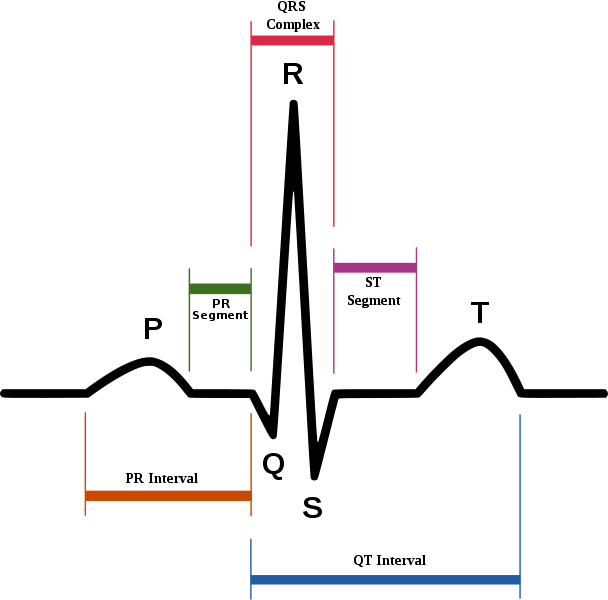
\includegraphics[scale=0.37]{./Abrak/Egyeb/ecg_wiki.png}
   \caption{Az EKG jel egy szívütése, illetve annak főbb diagnosztikai jellemzői.}
		\label{fig:ekg}
\end{center}
\end{figure}
 
Az irodalomban ismert tömörítő algoritmusokat \cite{unifiedReview} alapján három kategóriába sorolhatjuk: 1) egyszerű paraméteres becslések (pl.: interpoláció, különbségi kódolás, stb.), 2) direkt módszerek (pl.: csúcsok, meredekségek, stb. tárolása), 3) transzformációs eljárások. Az utóbbi osztály tartalmazza azokat az algoritmusokat, melyek a jelet egy előre adott függvényrendszer szerinti sorfejtéssel approximálják. Így az eredeti adatsorozat helyett csak az együtthatókat és a rendszer paramétereit kell tárolnunk. Ezen kategóriába sorolandó a dolgozatban bemutatott algoritmus is. Nevezetesen, az eredeti adatsorozatot speciális, Hermite-polinomok segítségével előállitott függvényrendszerrel fogjuk közelíti. A módszer alapját képező eljárás \cite{hexp3}, jól ismert az irodalomban, mely nem csak a jelek tömörítéséhez, de azok modellezéséhez \cite{hexp2}, illetve osztályozásához \cite{hexp1, hexp4} is alkalmazható. A dolgozatban az EKG jelekkel való hasonlóságuk miatt Hermite-függvényeket használunk az adatok reprezentálásához. Ezeket egy argumentum transzformáción keresztül szabad paraméterekkel egészítjük ki. Ennek köszönhetően az eredeti jelet egy adaptív bázisban írhatjuk fel. Az említett paraméterek megválasztásához a Nelder-Mead optimalizációs eljárást alkalmaztuk. Mivel az EKG jelek diszkrét adatsorozatok, ezért a módszert \cite{hexp5} alapján implementáltuk diszkrét ortogonális Hermite-polinomokra is. A dolgozatban különböző tesztekkel demonstráljuk az algoritmus hatékonyságát. Ehhez, több órányi, zajjal terhelt, valódi EKG felvételt használtunk. Ezen keresztül a bemutatott módszert összehasonlítottuk több másik, az irodalomban jól ismert tömörítő algoritmussal is \cite{jpeg2000ECG}. 

A tömörítő eljárást egy c++ nyelven megírt, objektum elvű alkalmazás implementálja, melyet egy webes felületen keresztül érhetünk el. A felület lehetőséget biztosít a dolgozatban jelölt tesztek újrafuttatására, valamint a teszteléskor felhasznált adatbázis további jeleinek a tömörítésére. Szintén a webes felületen keresztül nyílik alkamunk a már tömörített EKG jelek helyreállítására. 

Az alkalmazás megetrvezésekor külön hangsúlyt kapott a kód újra felhasználhatósága. Ennek érdekében a felhasznált algoritmusok, illetve matematikai modellek a lehető legáltalánosabb formában lettek implementálva. Fontos szempontot jelentett továbbá a c++11-es nyelvszabvány által nyújtotta lehetőségek minél hatékonyabb kihasználása. Jó példa erre a lambda függvények alkalmazása az optimalizációs algoritmusok implementációja során. A hatékony működés mellett azonban a program igyekszik megfelelni a modern felhasználók igényeinek. Ennek érdekében a felhaszálói felület weboldalként lett implementálva. A rendszerfüggetlen, és installáció mentes elérés lehetővé teszi a gyors és egyszerű használatot, valamint az eredmények megosztását.  

\section{Matematikai háttér}
\subsection{Jelek approximációja}

EKG jelek feldolgozásakor sok esetben szembesülünk gyakorlati kihívásokkal. Két sűrűn előforduló példa a hosszú mérések tárolása, valamint a zajjal terhelt mérések ábrázolása. Ezekre a nehézségekre egyszerre ad kielégítő megoldást, ha a jeleket  valamely $\mathcal H$ Hilbert-tér sima függvényeiből álló $(\Phi_n, n\in\Bbb N)$ ortogonális bázisában reprezentáljuk és a jelet véges sok $\Phi_0,\Phi_1,\cdots,\Phi_n$ bázisbeli elem lineáris kombinációjával közelítjük. Az $f\in\mathcal H$ jel
legjobb közelítését a tér $\|\cdot\|$ normájában az
$$
S_nf:=\sum_{k=0}^n\langle f,\Phi_k\rangle \Phi_k
$$
leképezés nyújtja, ahol $\langle\cdot,\cdot\rangle$ az $\mathcal  H$ tér
skaláris szorzatát jelöli. A jel és a közelítés eltérésének négyzete  a
$$
\|f-S_nf\|^2=\|f\|^2-\sum_{k=0}^n|\langle f,\Phi_k\rangle|^2
$$
képplettel adható meg. Adott hibán belüli közelítést véve a jel helyett  elég az
$S_nf$ approximációt reprezentáló  $\langle f,\Phi_k\rangle\ (k=0,1,\cdots, n)$ Fourier-együtthatókat tárolni.  Zajos jel esetén az ilyen típusú approximáció szűrőként is szolgál.  A közelítés megvalósításához a klasszikus ortogonális rendszerek közül  EKG görbék közelítésére  az Hermite-féle függvények bizonyultak használhatónak. Ezt támasztják alá a [...] dolgozatok. Az  Hermite függvények alkalmazása azzal is indikolható, hogy grafikonjuk hasonlít az EKG görbékre. Ezt a tulajdonságot a \ref{fig:phi0-3} ábra szemlélteti.

\iffalse

\begin{figure}
\centering
\subfigure[$\Phi_{0}(x)$]{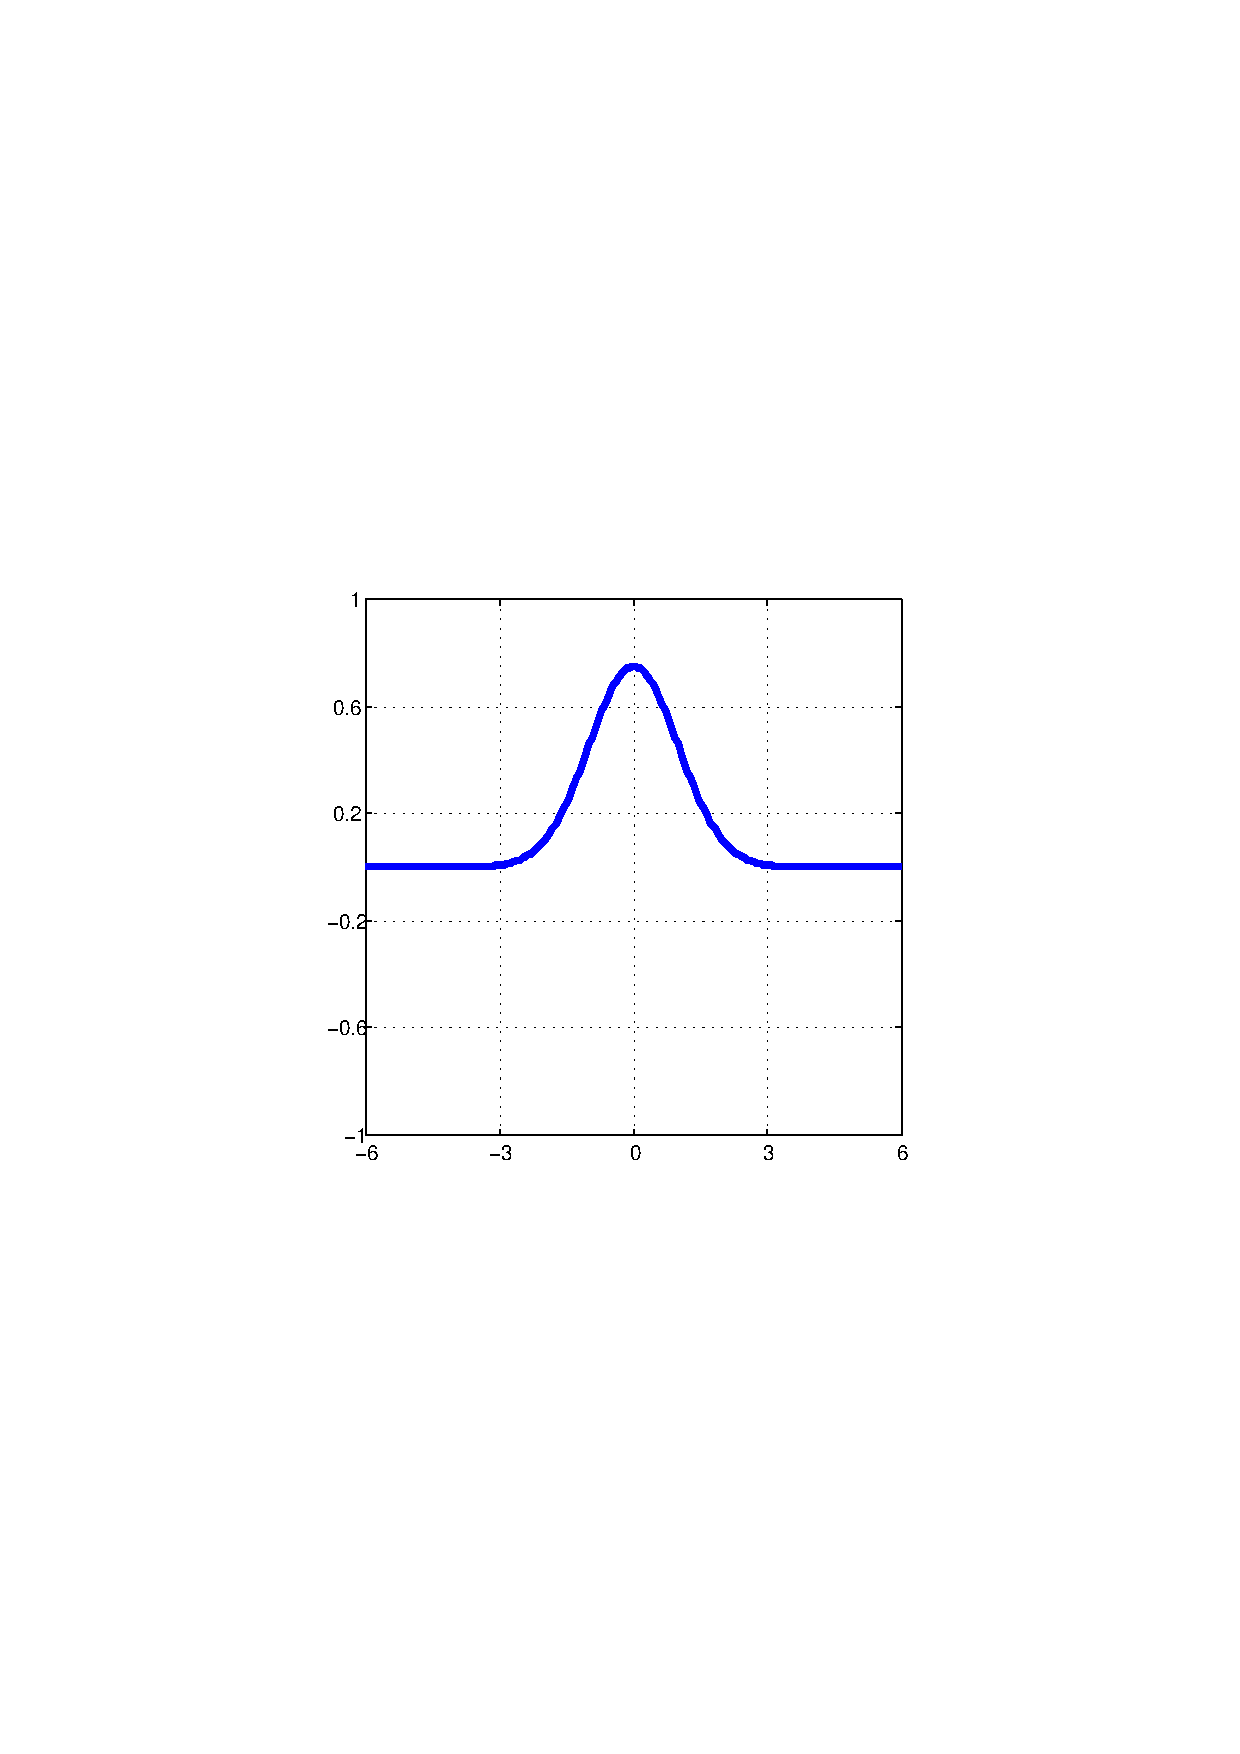
\includegraphics[scale=0.34,trim=150 280 150 280,clip]{./%Abrak/Egyeb/phi0.pdf}} 
\subfigure[$\Phi_{1}(x)$]{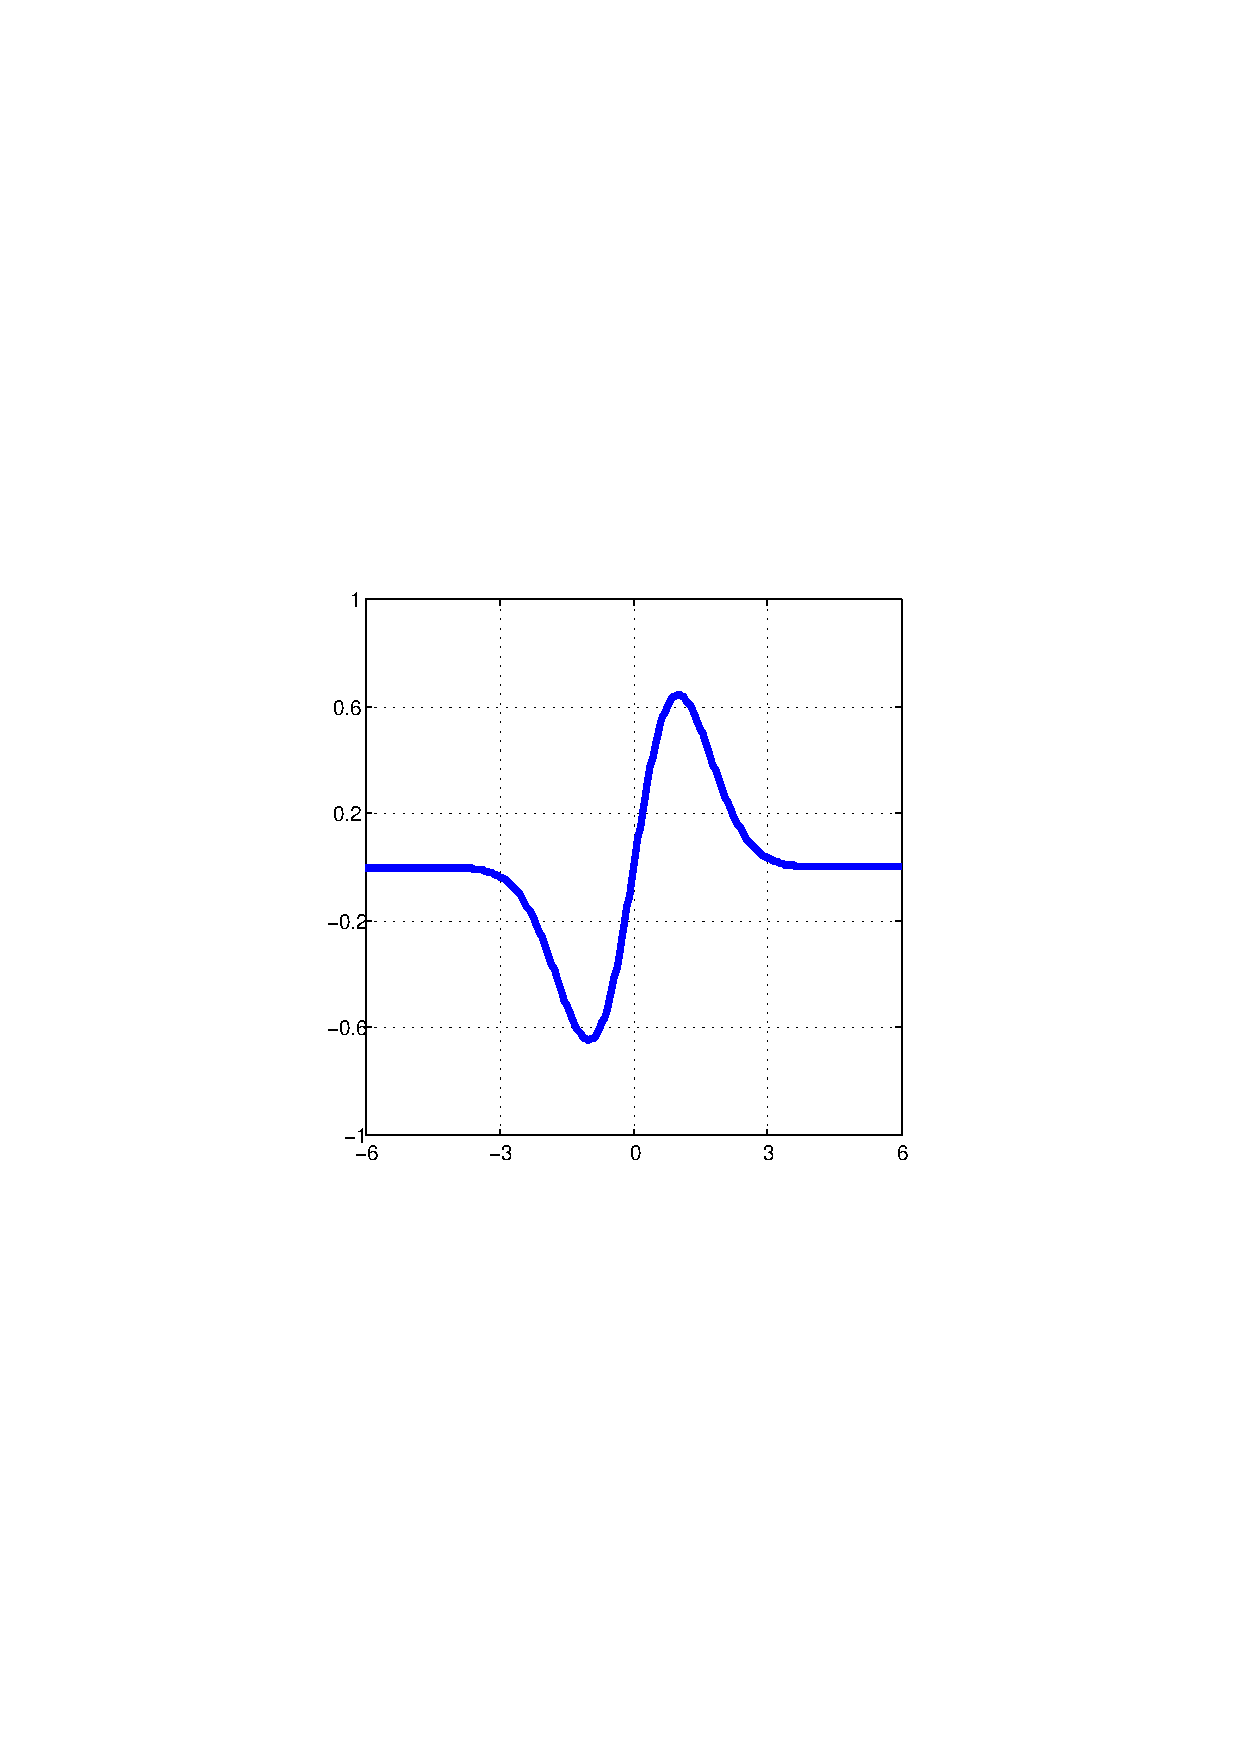
\includegraphics[scale=0.34,trim=150 280 150 280,clip]{./%Abrak/Egyeb/phi1.pdf}}
\subfigure[$\Phi_{2}(x)$]{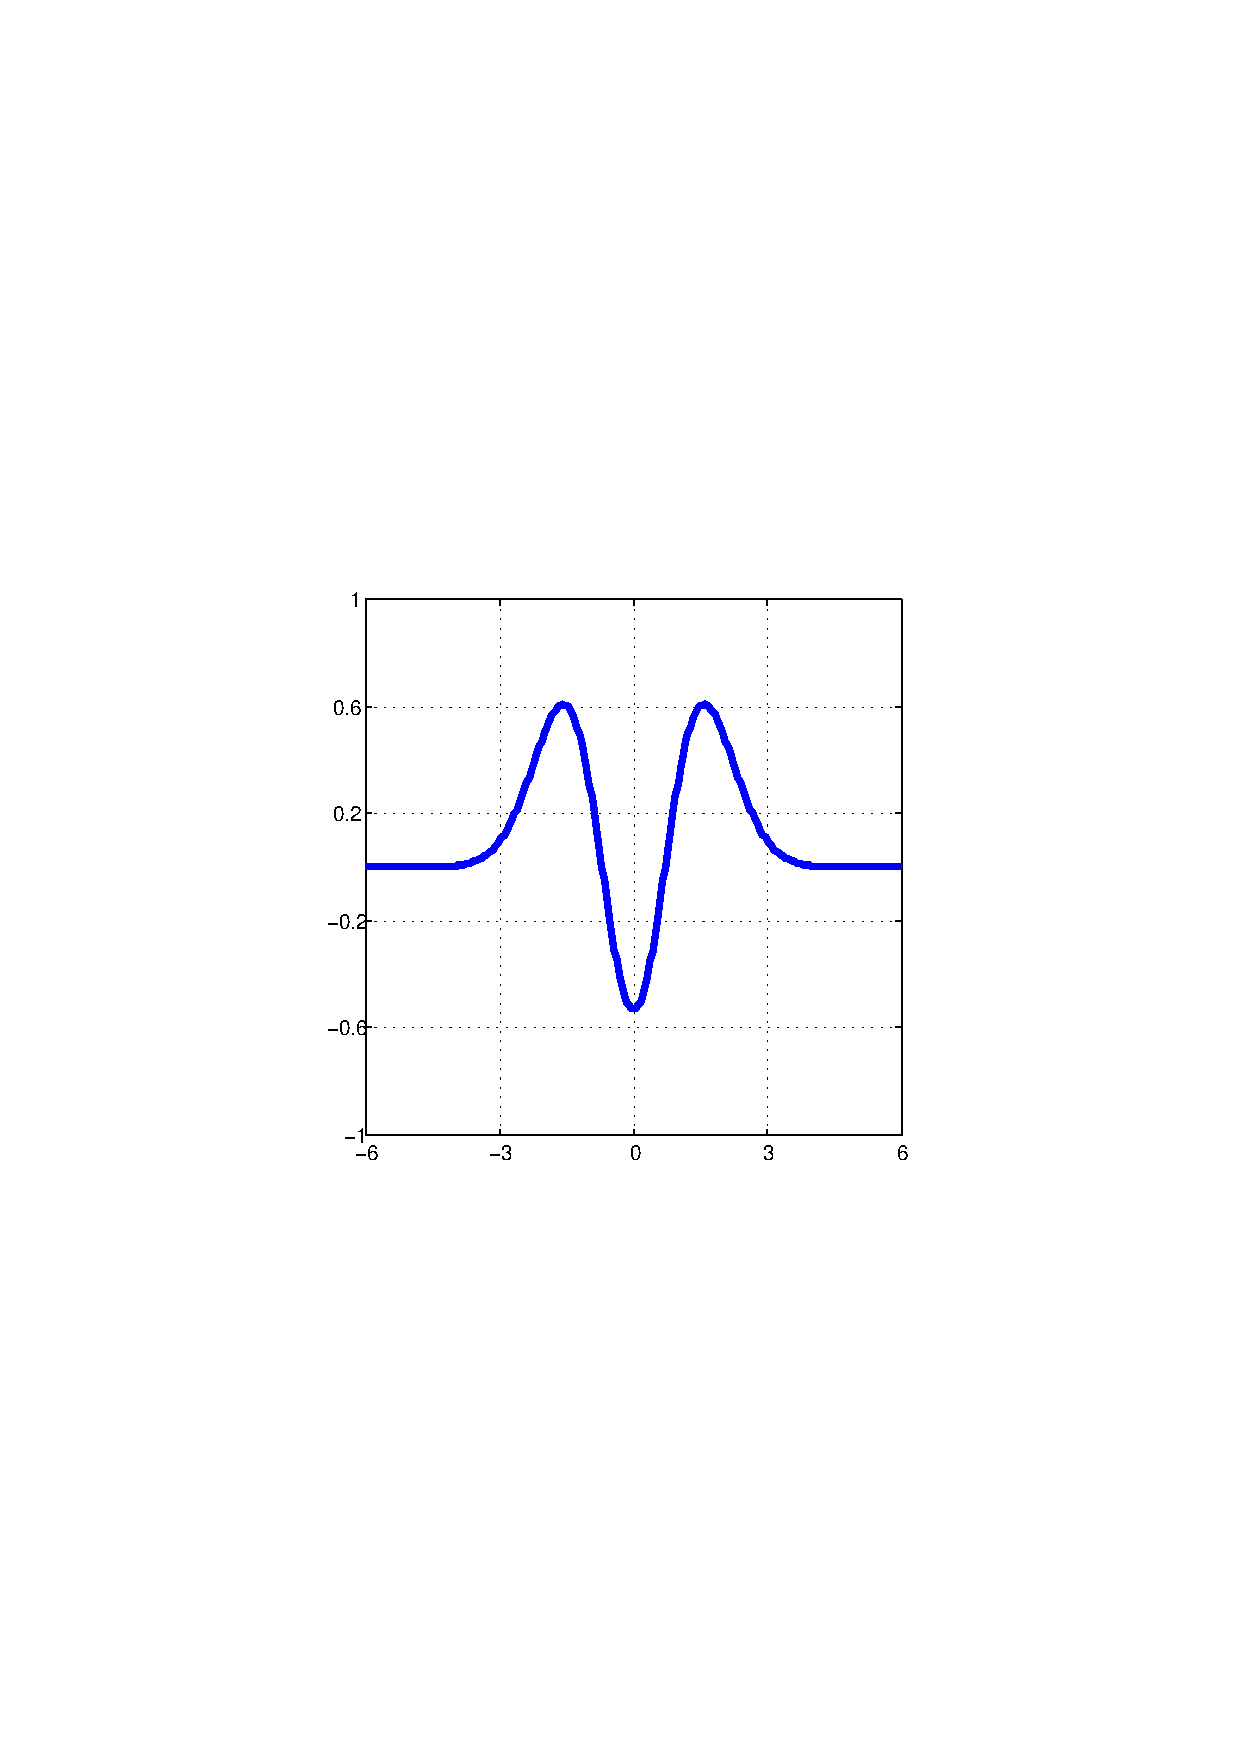
\includegraphics[scale=0.34,trim=150 280 150 280,clip]{./%Abrak/Egyeb/phi2.pdf}} 
\subfigure[$\Phi_{3}(x)$]{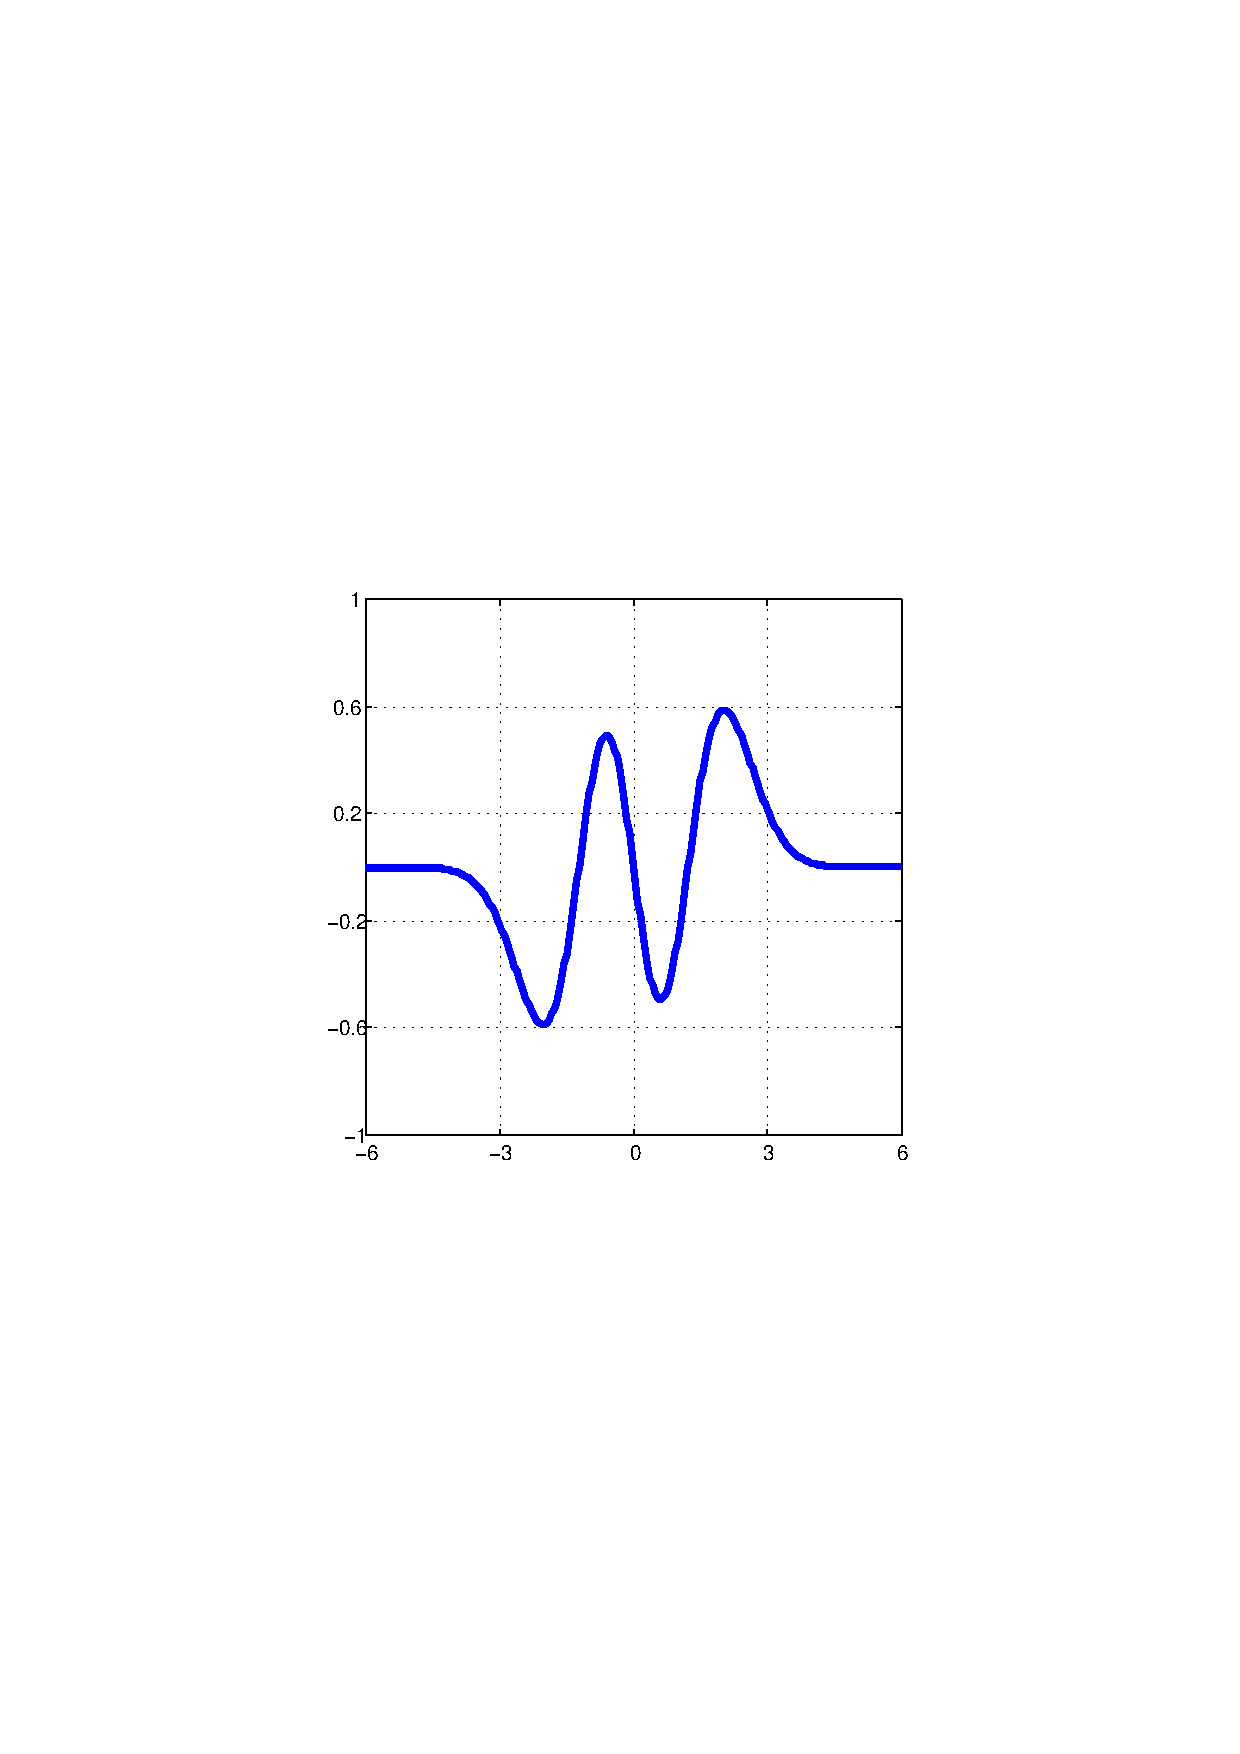
\includegraphics[scale=0.34,trim=150 280 150 280,clip]{./%Abrak/Egyeb/phi3.pdf}}
\caption{A Hermite-függvényrendszer első négy tagja.}
\label{fig:phi0-3}
\end{figure}
\fi


\subsection{Hermite-függvények}
A dolgozatban  az $\Bbb R$ számegyenesen (Lebesgue-mérték szerint) négyzetesen integrálható függvények $\mathcal H$ Hilbert-tere helyett elegendő a szakaszonként folytonos, az $\Bbb R$-en  négyzetesen integrálható függvények $\mathcal F$ euklideszi terét használni. Ebben a térben a skaláris szorzat és a norma a következő alakban írható fel:
\begin{equation}
 \langle f,g\rangle:=\int_{-\infty}^\infty f(t)g(t)\, dt,\ \ \|f\|:=\sqrt{\langle f,f\rangle}\ \ (f,g\in\mathcal F)\,.
\label{eq:dotprod}
\end{equation}
Továbbá, a
 \begin{equation*}
 \Phi_n(x):=H_n(x)e^{-x^2/2}/\sqrt{\pi^{1/2}2^n n!}\quad \ (n\in\Bbb N)
 \end{equation*}
normált Hermite-függvények (teljes) ortonormált rendszert alkotnak az $\mathcal F$ téren:
  \begin{equation*}
   \langle \Phi_n,\Phi_m\rangle=\delta_{nm}\ \ (m,n\in\Bbb N),\quad
  \|f-S_nf\|\to 0\ (n\to\infty)\,.
   \end{equation*}
Itt $H_n\ (n\in\Bbb N)$ jelöli az Hermite-féle polinomokat.
\\
\\
Az Hermite-függvények alkalmazásának számos előnye van: \\
\\
i) A $\Phi_n\ (n\in\Bbb N)$ rendszer zárt (teljes) az $\mathcal F$ téren. \\
\\
ii) A $\Phi_n(x)$ függvények gyorsan tartanak $0$-hoz, ha $|x|\to \infty$: \\
$$
|\Phi_n(x)|\le M_n e^{-x^2/4}\le M_n\ \ (x\in\Bbb R, n\in\Bbb N).
$$
\\
iii) A $\Phi_n$ függvények (stabil) másodrendű rekurzióval számíthatók: \\
\begin{equation}
\begin{split}
&\Phi_0(x):=e^{-x^2/2}/\pi^{1/4},\ \Phi_1(x):=\sqrt{2}\, x e^{-x^2/2}/\pi^{1/4}\\
&\Phi_n(x)=\sqrt{\frac 2 n} x \Phi_{n-1}(x)-\sqrt{\frac{n-1}n}\Phi_{n-2}(x)\ \ (x\in\Bbb R, n\ge 2)
\end{split}
\end{equation} 
\\
\\
iv) A $\Phi_n'$ deriváltak kifejezhetők a $\Phi_n, \Phi_{n-1} $ függvényekkel: \\
\begin{equation}
\Phi_n'(x)=\sqrt{2n}\Phi_{n-1}(x)-x\Phi_n(x)\ \ (x\in\Bbb R, n\in\Bbb N,\Phi_{-1}=0)
\end{equation}

\subsection{Az approximáció optimalizálása}

A jelek reprezentációja  függ az időskála $0$ pontjának és az egység
megválasztásától. Ezeket a paramétereket  a gyakorlatban önkényesen szoktuk
 megválasztani. Ezzel összefüggében felvethető a kérdés, hogyan lehet optimálisan megválaszthatani  ezeket a paramétereket.
Az  approximáció pontossága javítható azonos együttható szám mellett, amennyiben az  Hermite-függvények helyett azok
\begin{equation}
\Phi_n^{a,\lambda}(x):=\Phi_n(\lambda x+a)\ \  (x,a\in\Bbb R, \lambda>0)
\end{equation}
affin transzformáltjait használjuk. A $\sqrt{\lambda}\Phi_n^{a,\lambda}\ (n\in\Bbb N)$ rendszer is ortonormált és teljes az $\mathcal F$ téren. Ebben az esetben
az $f$ legjobb approximációja az
\begin{equation}
S_n^{a,\lambda}f:=\sum_{k=0}^n\langle f,\Phi_k^{a,\lambda}\rangle\Phi_k^{a,\lambda}\ \
(n\in\Bbb N, a\in\Bbb R,\lambda>0)
\end{equation}
projekció és a közelítés hibája az $a$ transzlációs és a $\lambda$ dilatációs paraméter függvénye:
\begin{equation}
D^2_n(a,\lambda):=\|f\|^2-\sum_{k=0}^n|\langle f,\Phi_k^{a,\lambda}\rangle|^2.
\end{equation}
            E két szabad paraméter optimalizálásával azonos együtthatószám mellett, az eredeti Hermite polinomokkal törtánő  approximációhoz képest pontosabb közelítés érhető el. A $D_n$ függvény minimalizálása ekvivalens  az
 $$
 F_n(a,\lambda):=\sum_{k=0}^n|\langle f,\Phi_k^{a,\lambda}\rangle|^2
 $$
 függvény maximumának meghatározásával. A paraméteres integrálok tulajdonságaiból következik, hogy az
 $$
 A_n(a,\lambda):=\langle f,\Phi_k^{a,\lambda}\rangle \ \  ((a,\lambda)\in T:=\Bbb R\times (0,\infty))
 $$
 Fourier-együtthatók a $T$ tartományon a paraméterek sima függvényei. Bebizonyítható, hogy $\lambda\to 0$ és $|a|+\lambda\to \infty$ esetén
 $F_k(a,\lambda)\to 0$, következésképpen az $F_n$ függvénynek létezik a
 maximuma és a $D_n$ függvénynek létezik a minimuma. A részleteket a Függelékben találhatók.

 Az alábbi ábrák az $F_n(a,\lambda)$ függvényeket szemléltetik fényintenzitás és perspektivikus ábrázolást használva. A harmadik ablakon
a jel közelí tését szemlélteti a maximum helynek megfelelő, ill.  egyéb
paraméter esetén.

\begin{figure}[H]
\begin{center}
   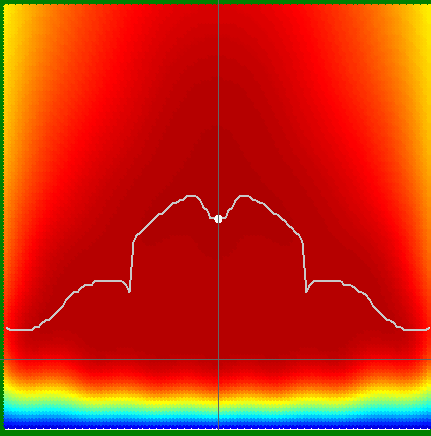
\includegraphics[width=100mm]{./Abrak/Ereszkedo1/F_2sz.png}
  \caption{Az $F_n$ szí nkódos ábrázolása}
\end{center}
\end{figure}

\begin{figure}[H]
\begin{center}
   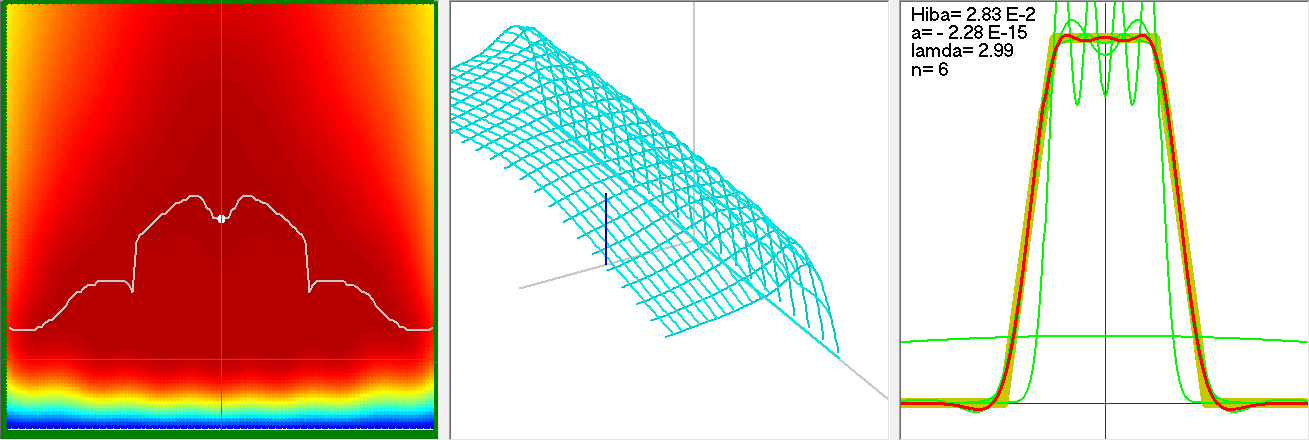
\includegraphics[width=140mm]{./Abrak/Ereszkedo1/Er36.png}
  \caption{Az $F_n$ által meghatározott felület, és approximáció}
\end{center}
\end{figure}

\section{A Nelder-Mead algoritmus}



A $Nelder-Mead$ szimplex algoritmust \cite{} eredetileg 1965-ben
fejlesztették ki azzal céllal, hogy létrehozzanak egy eljárást, amely
képes meghatározni egy $f : \Bbb R^n \to \Bbb R$ nemlineáris függvény minimum (maximum) helyét a  gradiens felhasználása  nélkül,
 pusztán a függvényértékekre  támszkodva. 
Mivel az algoritmust a bemutatott tömörítési eljárás során kétváltozós függvényekre kerül aklalmazásra, ezért ebben a speciális esetben szemléltetjük, megjegyezve, hogy hasonló 
elvek szerint
 működik az általános $n$ dimenziós eset is. Említendő továbbá, hogy Fejlesztői dokumentáció fejezetben bemutatott Nelder-Mead algoritmus implementációja képes kezelni az n-dimenziós esetet.  A minimum meghatározásához az $f(x_1), f(x_2), f(x_3)$  adnak kiindulási pontot, melyek közül egyet lecserélendő az adott lépésben. Nevezetesen, az algoritmus
\begin{equation*}
f(x_3)\le f(x_2)\le f(x_1)
\end{equation*}
 esetén olyan $x'$ helyet keres, amelyre $f(x')\le  f(x_3)\le f(x_2)$ teljesül és az $x_3, x_2, x_1$ ponthármasról az $x_1$-et elhagyva áttérünk az $x',x_3, x_2$ hármasra. Az $x'$ pontot az előzőekből geometriai transzformációkkal származtatjuk, felhasználva az  $x_2x_3$ szakasz $x=(x_2+x_3)/2$ felezéspontját: 
\begin{equation*}
x'=x_1+\alpha (x-x_1) \quad (\alpha\in\Bbb R)\,.
\end{equation*}
 Az alábbi ábrák szemléltetik az algoritmusban  használt transzformációkat. Látható, hogy $\alpha=2$ esetén $x'$ éppen az $x_1$ pont $x$-re vonatkozó középpontos tükrözése $(T_1).$ Továbbá $\alpha>2$ az eredeti háromszög tükrözése + nyújtása $(T_2),$ az $1<\alpha<2$ pedig tükrözéses + zsugorításnak felel meg $(T_3).$ A $-1<\alpha<0$ paraméterrel egyszerű zsugorítás adódik. Végül az 5. transzformáció $(T_5)$ az $x_3$ pontból történő
 kicsinyítésnek feleltethető meg. Az $x_1$ képe ezekben a transzformációkban és a hozzá tartozó függvényértékek a következő alakban adottak:
\begin{equation*}
x':=x_{3+i}=T_i(x_1)\quad (i=1,2,3,4), \qquad y_j=f(x_j)\quad (j=1,2,\cdots,7)\,.
\end{equation*}
Azt, hogy mikor melyik transzformáció használandó, a Függelékben, illetve a Fejlesztői dokumentáció Nelder-Mead algoritmus implementációjával foglalkozó fejezetben
található  folyamatábrából látható. Az említett műveleteket a \ref{fig:nmtrf} ábra szemlélteti.
\begin{figure}[htb!]
  \centering
\subfigure[Tükrözés\ $(T_1: \alpha=2).$]{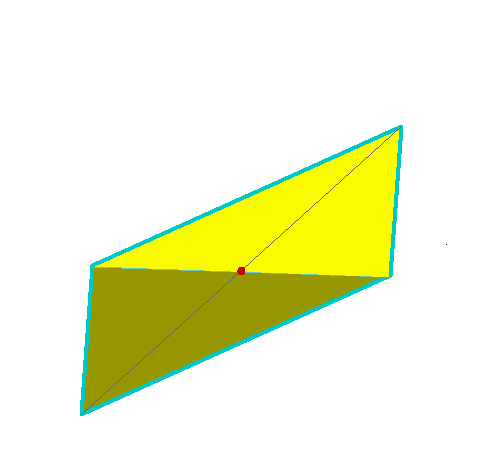
\includegraphics[scale=0.26,trim=10 0 10 53,clip]{./Abrak/Egyeb/NMT1.PNG}} 
\subfigure[T-Nyújtás\ $(T_2: \alpha=2.5).$]{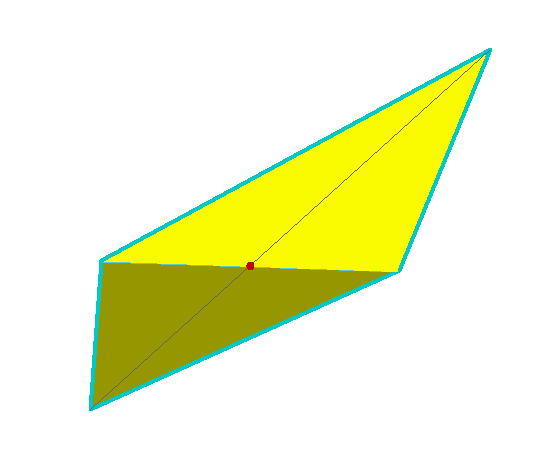
\includegraphics[scale=0.26,trim=10 0 10 53,clip]{./Abrak/Egyeb/NMT2.PNG}}
\subfigure[T-Összehúzás\  $(T_3:  \alpha=1.5).$]{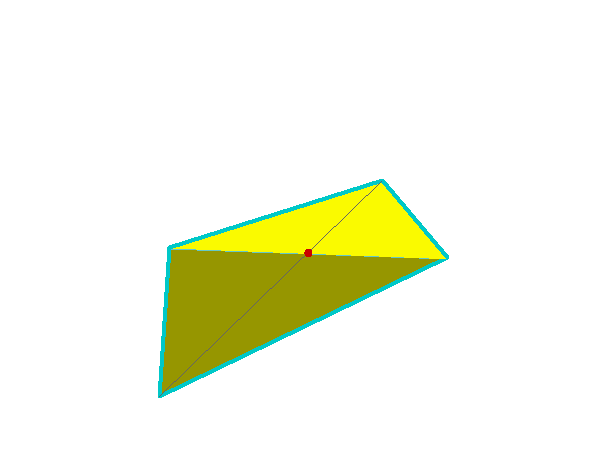
\includegraphics[scale=0.26,trim=10 0 10 53,clip]{./Abrak/Egyeb/NMT3.PNG}} 
\subfigure[Összehúzás\ $(T_4: -1<\alpha<0).$]{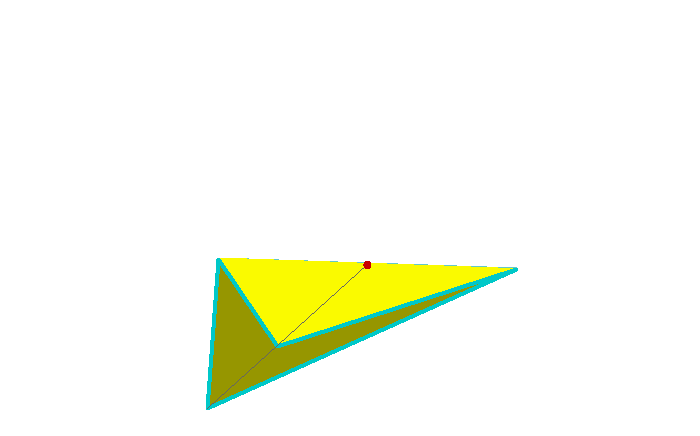
\includegraphics[scale=0.26,trim=10 0 10 185,clip]{./Abrak/Egyeb/NMT4.PNG}}
\subfigure[Kicsinyítés  $x_3$-ból $(T_5).$]{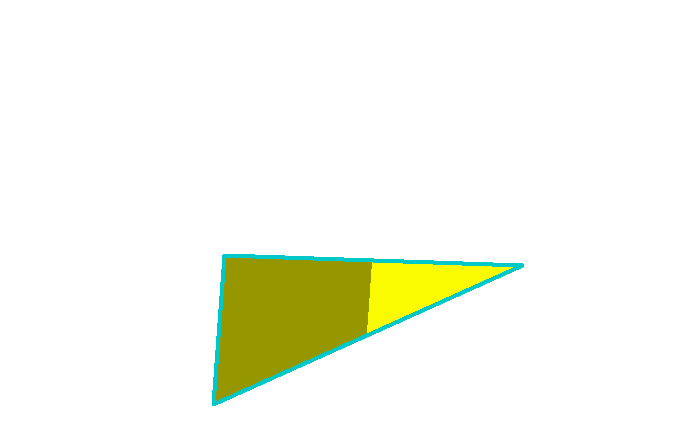
\includegraphics[scale=0.26,trim=10 0 10 185,clip]{./Abrak/Egyeb/NMT5.PNG}}
\caption{A $Nelder-Mead$ szimplex transzformációi.}
\label{fig:nmtrf}
\end{figure}

Megjegyezendő, hogy a $Nelder-Mead$ szimplex módszer egy determinisztikus algoritmus. Az algoritmus gyors, hiszen minden lépésben csak néhány függvénykiértékelést kell végezni. Továbbá, egyes módszerek, például a gradiens módszerrel ellentétben az olyan patologikus függvények optimumát is képes gyorsan megtalálni, mint amilyen a Rosenbrock függvény. 

\section{Kvadratúra formulák}


Mivel a $Nelder-Mead$ algoritmus
kizárólag a függvényértékekre támaszkodik, a hibafüggvény értékeinek kiszámításához elegendő az Hermite-függvényeket valamilyen felosztás pontjaiban egyszer meghatatározni. Ez implementációs szempontból is fontos, hiszen nem kell minden $(\lambda,a)$ paraméterhez kiszámolni az ettől függő, rekurzióval adott Hermite-féle függvényrendszer tagjait. Ehelyett elég az eredeti diszkrét adatsorozatot dilatálni, illetve eltolni, ami lényegesen kevesebb számítást igényel. Továbbá, az említett felosztás pontjainak valamely Hermite-függvény zérushelyeit választva, a hibafüggvényben  szereplő integrálok kiszámításához
a \cite{} dolgozatban használt eljáráshoz hasonlóan kvadratúra formulát is alkalmazhatunk. Ennek előnye, hogy az alappontokban a módszer interpolál, így itt lehetséges a jel mintáinak pontos rekonstrukciója. Ugyanakkor, a kapott approximáció is pontosabb, amit a \cite{}-ben közölt numerikus tesztek is alátámasztanak.
	\par Ahogyan ez a \cite{} dolgozatban látható, további optimalizációs algoritmusok is alkalmazhatóak a probléma megoldásához. Egy ezek közül a leggyosrabb ereszkedés módszere, melynek az alkalmazásához 
szükségünk van a függvény parciális deriváltjaira. Ezek előállításával ilyen esetben
külön  kell foglalkozni. Az Hermite-függvények deriváltjaira vonatkozó formulák alapján a
parciális deriváltakra a hibafüggvényhez hasonló ellőállítás adható. Ebben az esetben az \eqref{eq:dotprod} egyenletben szereplő integrálok kiszámításához ekvidisztans felosztása alkalmazandó.


\section{A tömörítő eljárás jellemzése}



A tömörítés kezdetekor az első feladat a teljes EKG mérést szívütésekre bontása. Ezt követően
az egyes szívütések a tömörítő eljárás bemeneti paramétereként válnak értelmezhetővé. Inicializálni kell továbbá
a tömörítő függvények által visszaadott, az aktuális szívütésre vonatkozó Fourier-együtthatókat, 
az approximáció hibáját, illetve az optimalizációs eljárások által meghatározott dilatációs és 
transzlációs paramétereket. \par
	
A tömörítés előkészítése nem ér véget a jel szívütésekre történő felbontásakor. A szívütéseket normalizálása is szükséges. Ez azt jelenti, hogy az első és utolsó helyen felvett értékeket összekötő egyenes, és az eredeti EKG különbségét tekinti az eljárás tömörítendő jelnek. Ezt az eljárást az irodalomban az alapvonal eliminálásnak nevezik. Ennek eredményeként a jel tartója a kezdő és a végpont által meghatározott intervallum. Végül, a szívütést normálásra kerül, vagyis az egyes értékeket 
elosztjuk az abszolút maximummal. \par
	A tömörítés megkezdése előtt inicializálni kell a függvényrendszert, 
melynek során az egyes bázisfüggvények által felvett értékek egy mátrix soraiba kerülnek: 
\begin{equation*}
	\Phi:=\left[\Phi_n(\alpha_m)\right]_{0\leq n < N,\;0\leq m < M}\,.
	\label{eq:phi_matrix}
\end{equation*}
A $\Phi\in\mathbb{R}^{N\times M}$ mátrix segítségével az $f\in\mathbb{R}^M$ diszkrét jel Fourier-együtthatói könnyen meghatározhatók:
\begin{equation*}
	c_n:=\left\langle f, \Phi_n \right\rangle=\frac{1}{M} \Lambda^{-1} \Phi f \quad (0\leq n < N)\,,
	\label{eq:phi_coeffs}
\end{equation*}
ahol $\mathbb{R}^{N\times N}\ni\Lambda=\Phi \Phi^T$ Cristoffel-Darboux számokat tartalmazza. Az előállításban szereplő $\alpha_n\in\mathbb{R}\, (0\leq n < N)$ számok a \ref{sec:kvad} fejezetnek megfelelően kétféleképpen határozhatóak meg. Egyrészt a $Nelder-Mead$ algoritmusban a $\Phi_N$ függvény gyökeit véve kvadratúra formulákat definiáltunk. Más optimalizációs algoritmusok, például a gradiens módszer esetén $f$ tartóján egyenletes alapponterndszert alkalmazandó. Figyelmet érdemel, hogy az előbbi esetben a gyökök pontos meghatározása kritikus a feladat szempontjából. A probléma megoldásához a \cite{gautschi} könyv által javasolt numerikus eljárás található az implementációban. Nevezetesen, a $H_n$ Hermite-polinom \eqref{eq:identities} rekurziójában szereplő együtthatókat egy tridiagonális mátrixba rendezzük. Könnyen belátható, hogy az $\alpha_n$ gyökök megegyeznek ezen tridiagonális mátrix sajátértékeivel.  \par

Hátra van még a megfelelő $(a,\lambda)$ paraméterek beállítása. Annak érdekében, hogy a reprezentáció minél adaptívabb legyen, több  optimális transzláció, illetve dilatáció meghatározása szükséges. Az eredeti $f\in\mathcal{F}$ jelet tehát a következő alakban közelíti a módszer:
\begin{equation*}
	S_{\mathbf{n}}^{\mathbf{a},\boldsymbol{\lambda}}f:=\sum_{i=1}^N\sum_{k=0}^{n_i} \langle f^{a_i,\lambda_i},\Phi_{k}\rangle\Phi_{k} \quad
	(a_k \in \Bbb R,\lambda_k>0)\,,
\end{equation*}
ahol $\mathbf{a}=a_1, a_2, \ldots, a_N$ az alkalmazott transzlációk, $\boldsymbol{\lambda}=\lambda_1, \lambda_2, \ldots, \lambda_N$ pedig a dilatációk sorozata. Az egyes sorfejtésekhez tartozó együtthatók számát az $\mathbf{n}=n_1, n_2, \ldots, n_N$ vektor jelöli. Mivel az EKG jel alapvetően három fő hullámból áll ezért jelen probléma megoldásakor $N=3.$ Továbbá a \cite{hexp3} dolgozat eredményei alapján
a QRS komplexumot egy heted, a T hullámot hatod, a P hullámot pedig egy másodfokú ortogonális rendszer segítségével approximálja az eljárás azaz $\mathbf{n}=7,6,2\,.$ Fontos, hogy a legjobb approximáció előállításához a \eqref{eq:hilaprx} egyenlettel ellentétben már az eredeti függvény $f^{a_i,\lambda_i}$ transzformáltja használatos. Ez nem jelent megszorítást az eredeti problémára nézve, implementációs szempontból viszont $f^{a_i,\lambda_i}$ kiszámítása gyorsabb, mint a $\Phi_n^{a_i,\lambda_i}$ rendszer előállítása.

A $(a_i,\lambda_i)$ paraméter párok optimalizációja egymástól függetlenül történik. Így azonban nem garantált, hogy az algoritmus a P, QRS, T hullámokat külön-külön approximálja. A problémát az irodalomban jól ismert ún. $Matching\ Pursuit$ $(MP)$ konstrukció \cite{mpurs} alkalmazásával oldja meg a módszer. Ez egy mohó algoritmus, mely minden lépésben a \eqref{eq:Fnfuggv} egyenletben definiált $F_n(a_i,\lambda_i)$ függvény maximalizálására törekszik. Az iteráció $i.$ lépése a következő alakban írható fel:
\begin{equation}
	s^{(i)}=s^{(i-1)} + S^{a_i,\lambda_i}_{n_i} R^{(i-1)} \quad (1\leq i \leq N)\,,
\label{eq:mpurs}
\end{equation}
ahol $R^{(i)}=f-s^{(i)}$ a rezidum függvényt jelöli. Röviden tehát az $s^{(0)}=0,\ R^{(0)}=f$ inicializálás után, az eljárás az $i.$ lépésében megkeresi az $R^{(i-1)}$ függvény $\ell^2$ norma szerinti legjobb közelítését, amit ki is von az említett rezidum vektorból. Ezt $N$ iteráción keresztül ismétli az aktuális $R^{(i)}$ függvényre. Az MP módszer egy gyors algoritmus, mellyel megkonstruálható az $f\in\mathcal{F}$ jel ritka reprezentációja. Emellett lehetséges az EKG szívütéseinek automatikus szeparációja is, hiszen a jel különböző részeit eltérő ortogonális rendszerek segítségével közelítjük. Figyelmet érdemel, hogy az eredeti \cite{hexp3} módszerben ezt a lépést egy külön szegmentáló algoritmus végezte. Így a közelítés pontossága erősen függött a szegmentálás eredményétől (lsd. \ref{sec:test} fejezet). A kifejlesztett eljárásnál azonban ez a probléma nem áll fenn még zajos jelek esetén sem. A dolgozatban bemutatott módszer iterációs lépéseit, az $R^{(i)}$ rezidum függvények alakulását, illetve a szeparált EKG jelet az \ref{fig:mpstep} ábra szemlélteti. Jól látható az is, hogy a fekete vonallal jelölt optimális transzláció általában nem az abszolút maximum helyén található. Ez indokolja, hogy a $\lambda_i$ dilatáció mellett az $a_i$ paraméter optimalizációjára is szükség van. Mivel ez utóbbi a kiindulásként használt \cite{hexp3} dolgozatból hiányzik, ezért a pontosság és tömörítési arány jelentős javulása várható el tőle.
\begin{figure}[htb!]
  \centering
\subfigure[A QRS approximációja.]{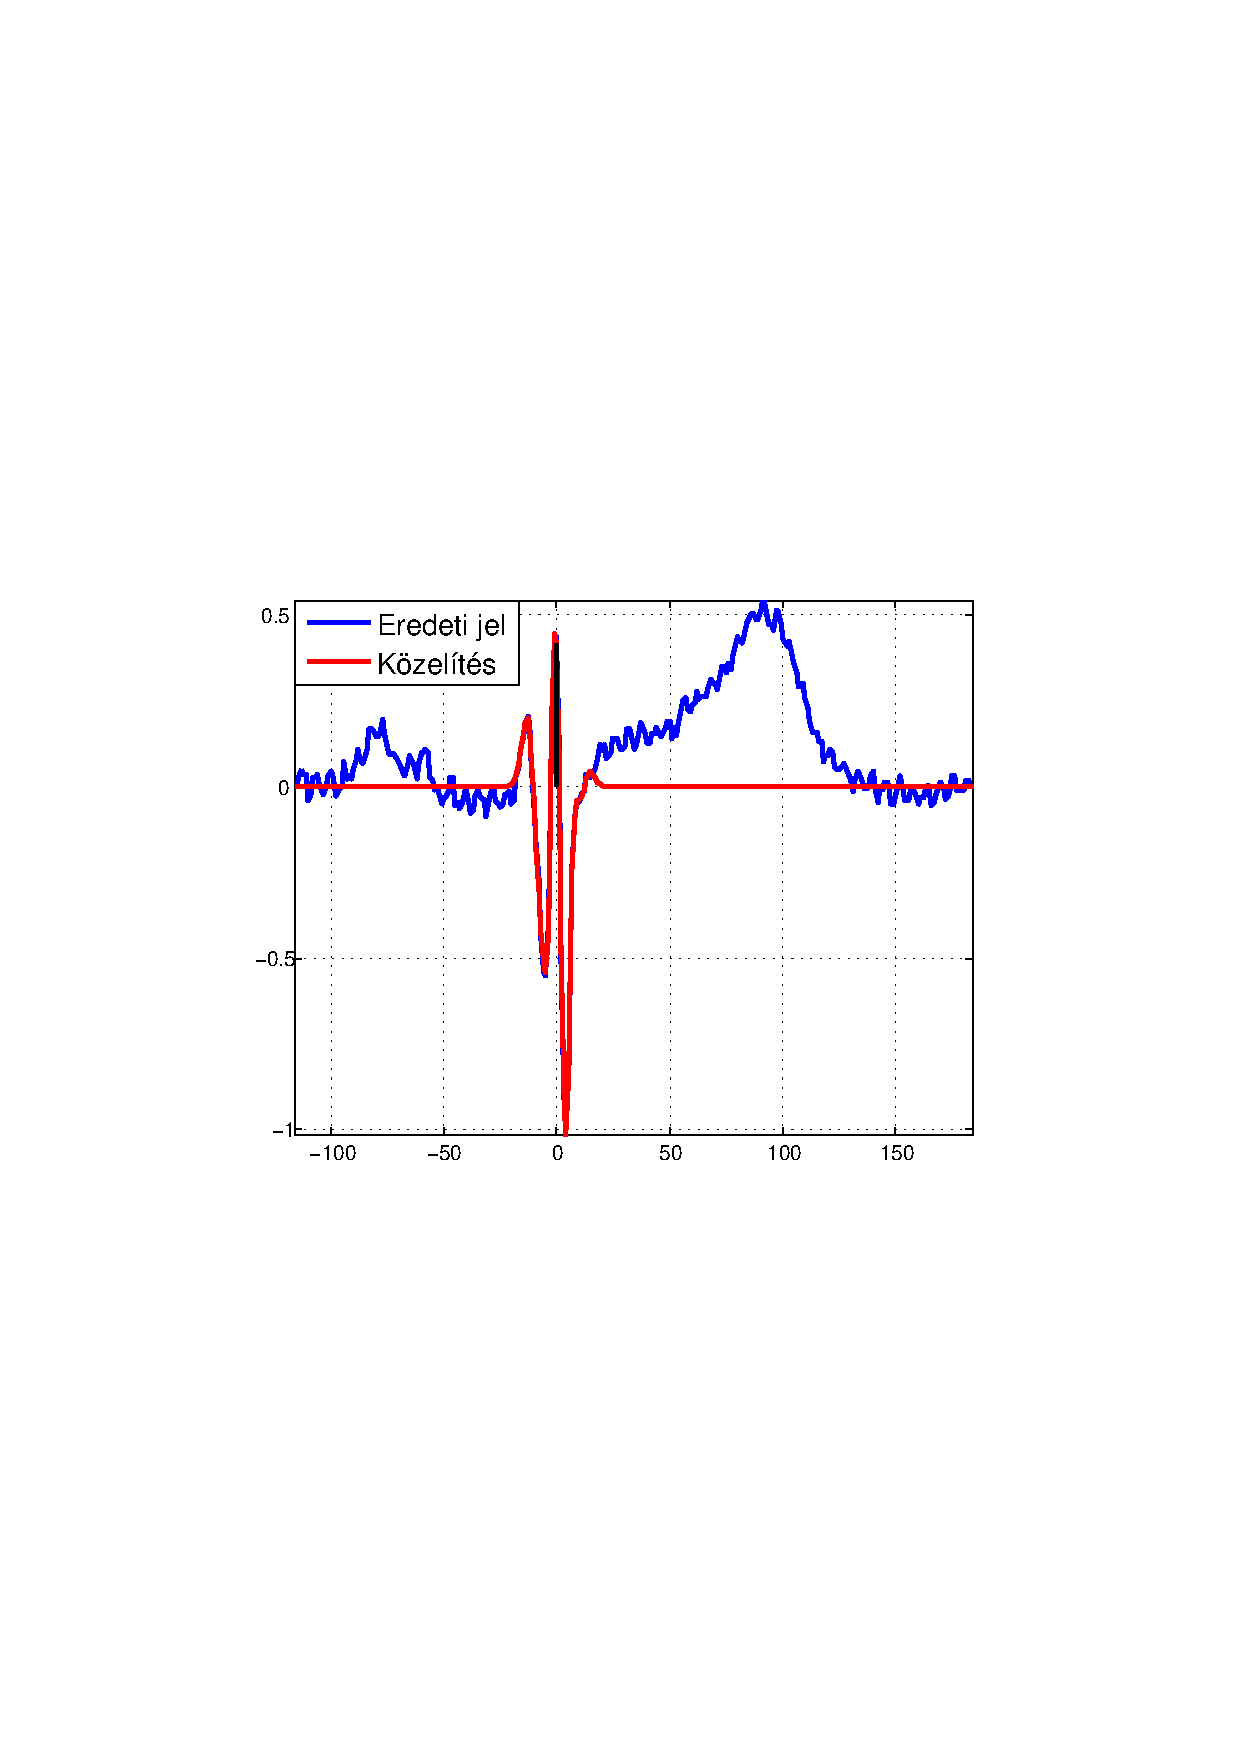
\includegraphics[scale=0.5,trim=120 280 100 280,clip]{./Abrak/Lepesek/abra_lepes0.pdf}} 
\subfigure[A T hullám approximációja.]{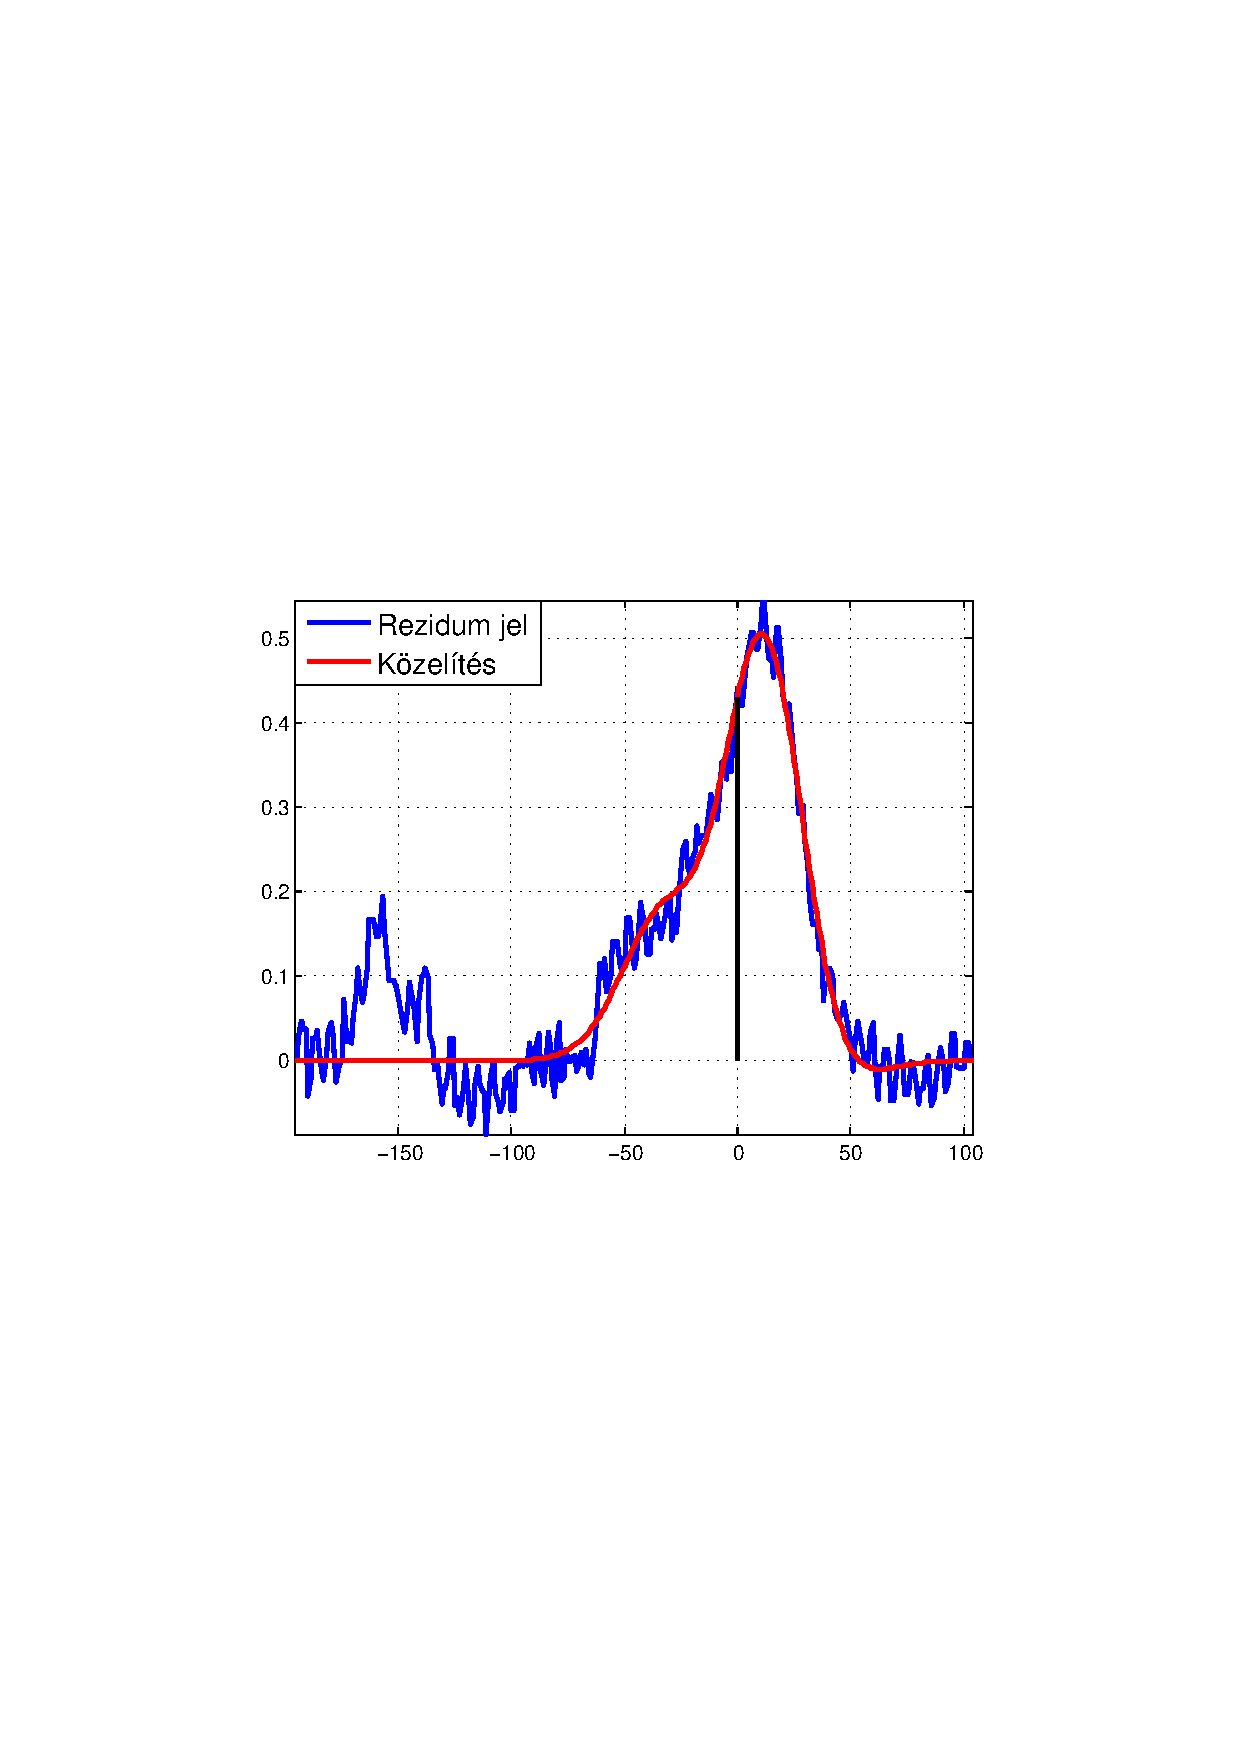
\includegraphics[scale=0.5,trim=120 280 100 280,clip]{./Abrak/Lepesek/abra_lepes1.pdf}}
\subfigure[A P hullám approximációja.]{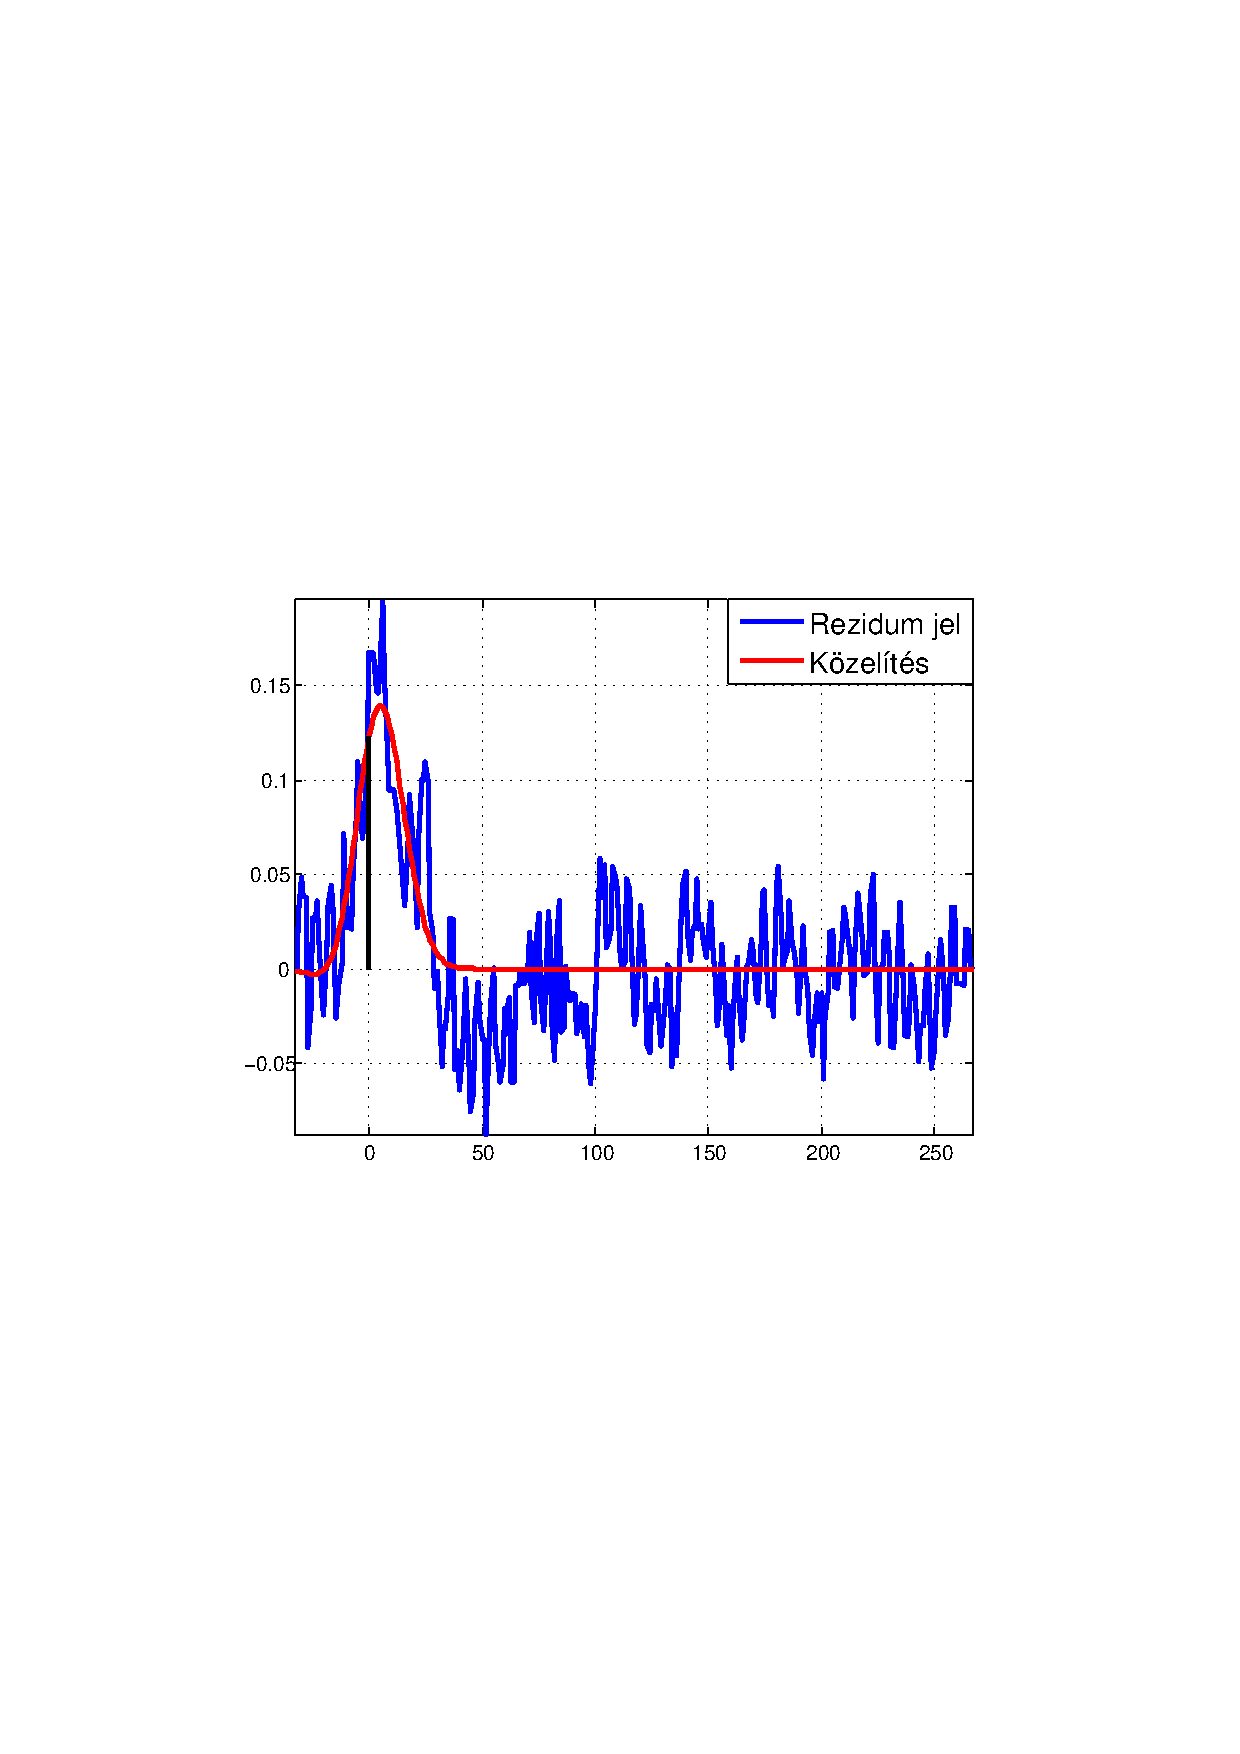
\includegraphics[scale=0.5,trim=120 280 100 280,clip]{./Abrak/Lepesek/abra_lepes2.pdf}} 
\subfigure[Szeparált szívütés.]{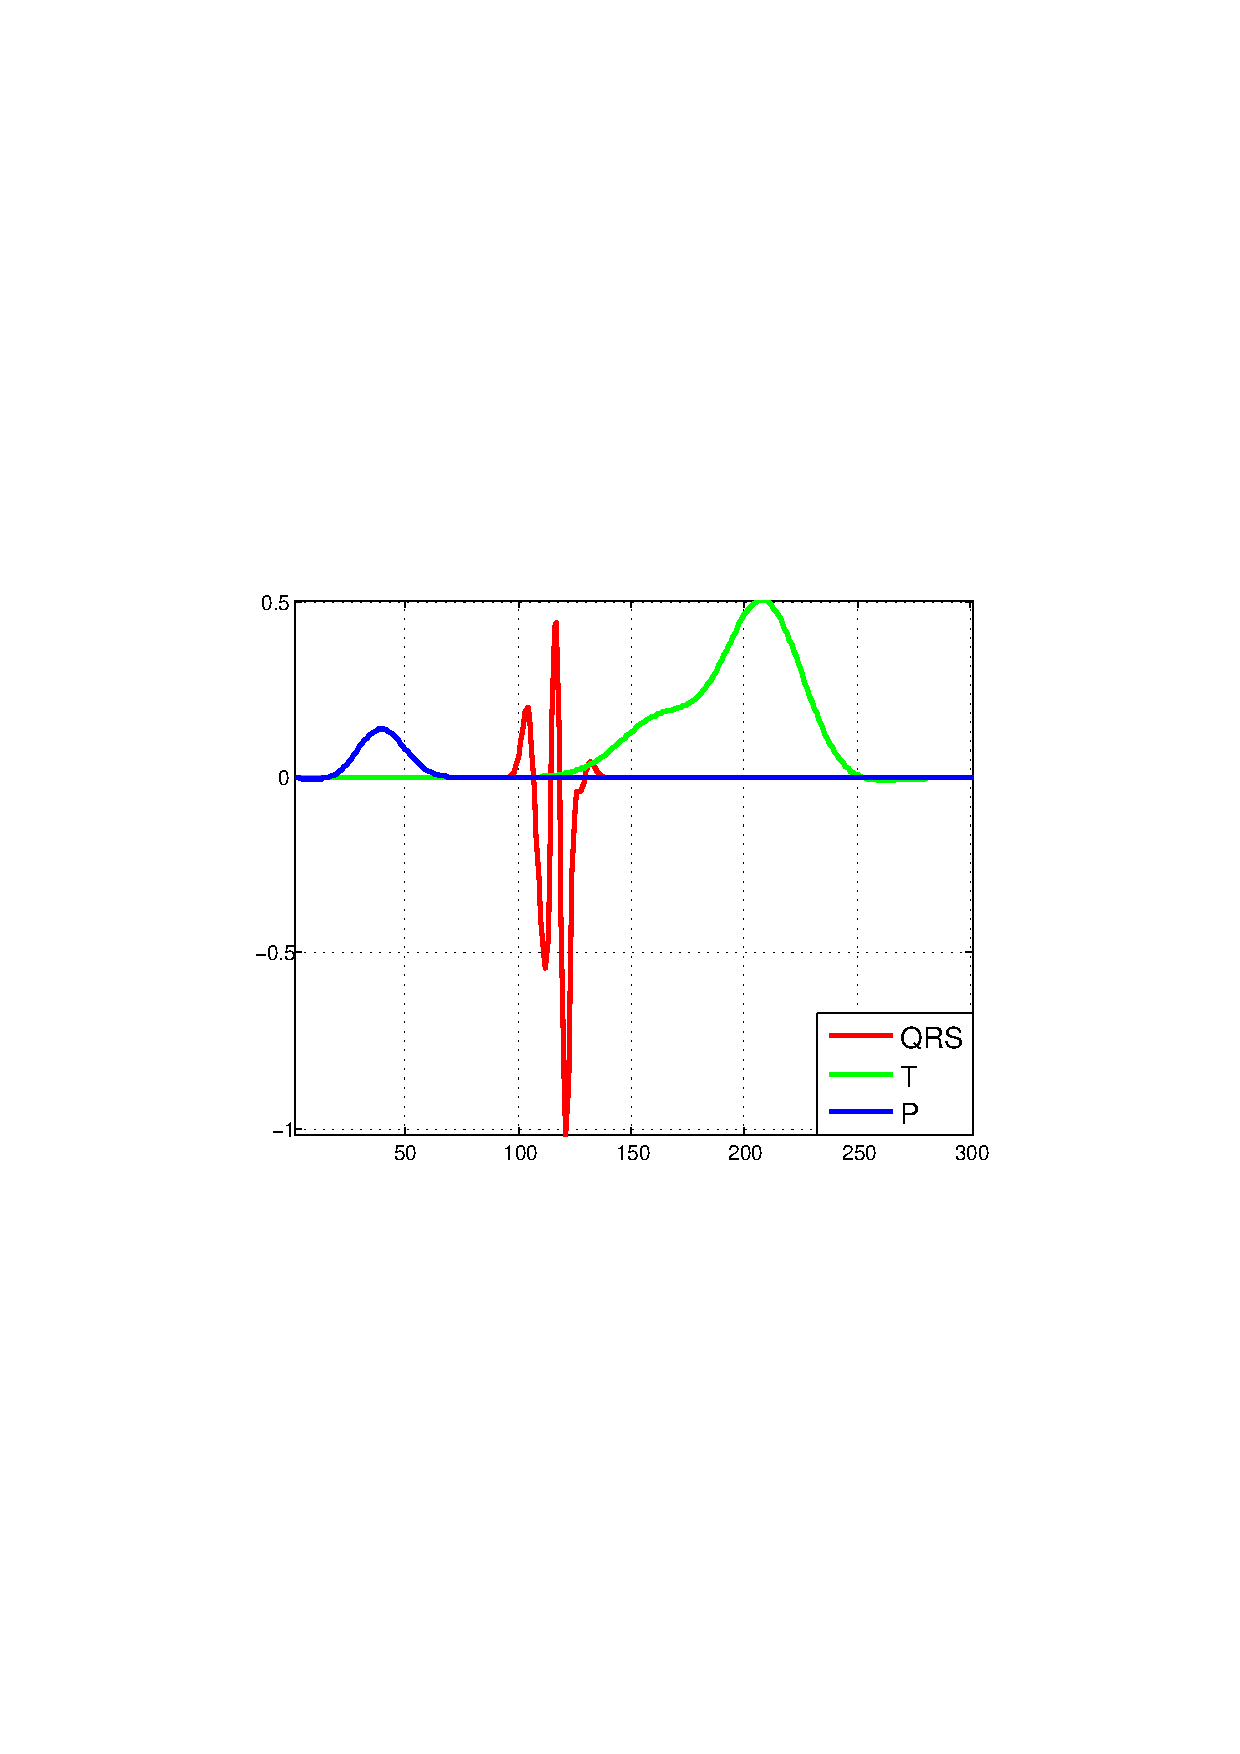
\includegraphics[scale=0.5,trim=120 280 100 280,clip]{./Abrak/Lepesek/abra_lepes3.pdf}}
\caption{Az MP algoritmus lépései.}
\label{fig:mpstep}
\end{figure}


\chapter{Felhasználói dokumentáció}

\chapter{Fejlesztői dokumentáció}

Ebben a fejezetben található a Bevezetés-ben bemutatott eljárás implementációjának pontos (modul szintű) leírása, valamint az alkalmazott tesztek jellemzése illetve ezek eredményei. A tesztelés eredményeit a tapasztalok összegzése és néhány lehetséges jövőbeli fejlesztés jellemzése követi. \par A fejlesztői dokumentáció első részében a tömörítési módszer implementációjának leírása található. Ez az alfejezet két fő részre tagolható: a webes felhasználói felület és az ehhez felhasznált könyvtárakat leíró, valamint a háttérben a konkrét tömörítést elvégző c++ program modulonkénti jellemzését. Mivel a webes felület megvalósítása rövid, és specializált scriptek összessége, ezért ezek jellemzését minden esetben egyedi módon érdemes kezelni. Ellentétben ezzel a szemlélettel, a c++ program nagyban épít a nyelv által támogatott objektum orientált megközelítésre. Ez lehetővé teszi és indokolja is egyben, hogy az implementációt jellemző dokumentáció is hasonlóan jól strukturált legyen. Az egyes modulok dokumentációja ugyanazon három szempont szerint közelíti meg a jellemzésüket: a modul feladatának, a modul interfészének (hogyan és mely egyéb modulokhoz kapcsolódik), valamint a modult felépítő osztályok implementációjának pontos megfogalmazása. A modulok leírásánál találhatóak továbbá a szemléltetést segítő UML és egyéb hasznos diagrammok. 
\par  A teszteléssel foglalkozó alfejezet szintén több részre tagolható. Az első alfelejezetben található a webes felhasználói felület funkcióinak tesztelési terve, illetve az egyes tesztek eredményeinek leírása. Ezt követi a c++ program moduljainak részletes tesztelési terve. A modulok tesztelését minden esetben egy külön tesztfájl végezte. Ennek leírása, az eredmények értékelése, illetve a tesztállomány elérési útja szintén megtalálható az alfejezetben. A  tesztelés alfejezet utolsó része a bemutatott tömörítési eljárást hivatott tesztelni. Ez több szempont alapján, egyéb EKG tömörítő módszerekkel történő összehasonlítás útján valósul meg. 

\section{A felhasználói felület implementációja}

A fejezet fő célja a webes felhasználói felületet feladatainak specifikációja, és a felületet alkotó scriptek belső felépítésének jellemzése. A fejezet elején található a webes felület specifikációja, amely pontosan meghatározza a felülettel szemben állított elvárásokat. Az implementációt tárgyaló egyes alfejezetek két típusra bonthatóak. Először is azoknak a .php kiterjetsztésű állományoknak a dokumentációja következik, amelyekkel a felhasználó közvetlenül érintkezik. Ez azt jelenti, hogy ezen állományok alkotják a programcsomag vizuális elemeit, illetve itt kerülnek meghatározásra a felhasználók által igénybe vehető bemeneti és kimeneti szolgáltatások. A fejezet második felében kerülnek tárgyalásra azok a scriptek, amelyekkel a felhasználó nem kerül közvetlen kapcsolatba. Ezek a rövid programok biztosítják a kapcsolatot a felhasználói felület és a jelfeldolgozást végző c++ alapú programcsomag között. A fejezet legvégén található a kakukktojásnak mondható \texttt{build\_all.sh} script jellemzése, melynek segítségével egyszerűen megépíthető és felkonfigurálható a programcsomag. 

\subsection{A felhasználói felület specifikációja}

A felhasználói felülettel szemben alkotott elvárásokat meg kell feleltetni a dolgozat elején, a \ref{specifikáció} fejezetben található egész programcsomagra vonatkozó elvárásoknak. Ezt leszögezve azonban fontos rámutatni, hogy egy teljes, sok tízezer mintából álló mérés tömörítése nagyon időigényes művelet, a webes felhasználói felület elsődleges célja pedig, hogy a c++ nyelven írt fő program tömörítési, illetve kitömörítési funkcióinak meglétét, illetve helyességét igazolja. Ezt a célját a felület akkor is eléri, ha nem ad szabadkezet a felhasználónak abban, hogy mely adatbázisbeli jelek mely konkrét szívütéseit tömörítse, hanem a tömöríthető jeleket a \ref{összesített táblázat} fejezetben található táblázat méréseinek első három szívütésében határozza meg. Természetesen a fő programcsomag alkamas az MIT-BIH adatbázisban található bármely teljes mérés tömörítésére is, azonban ezt a jelenlegi implementáció kizárólag manuális indítással teszi lehetővé \ref{felhasználói doksi, hosszú jelek tömörítése}. Ez a fajta korlátozás lehetővé teszi, hogy a webes felhasználói felület által nyújtott proof of concept szolgáltatások élvezhetőek maradjanak a felhasználók számára. 
\par Az eddig ismeretett fő irányelvek ismeretében összefoglalhatóak a legfontosabb elvárások a webes felhasználói felülettel szemben, melyek egyben annak a specifikációját is adják:
\begin{itemize}
  \item A webes felület feladata, hogy vizuálisan ismertesse egy konkrét szívütés tömörítésének menetét.
  \item A webes felület feladata, hogy bemutassa a fő c++ program tömörítési képességét, vagyis az elérhető jelek bármelyikének első három szívütését tömörítse. A tömörítés során létrejött .cmp szöveges állományt (amely a szívütések tömörített alakját tartalmazza), letöltésre elérhetővé kell tennie a felhasználó számára. 
  \item A felhasználói webes felületnek biztosítania kell, hogy a felhasználó a szerverre feltölthesse a birtokában lévő .cmp állományokat. Az ezekben található tömörített szívütéseket továbbítania kell a fő program részére, hogy az a kitömörítést elvégezhesse. A kitömörítés során a keletkezett jelek mintái egy szöveges állományba kerülnek, melynek elérhetővé tétele a webes felhasználói felület feladata.
  \item A webes felületnek rövid jellemzést kell adnia a bemutatott módszerről, illetve az elérhető szolgáltatásokról. 
\end{itemize}
   
A továbbiakban a webes felület alkotó scriptek egyenkénti jellemzése következik. Az itt ismertett scriptek és állományok a \texttt{/www/szd} útvonalon érhetőek el. 

\subsection{Az about.php implementációja}

Az \texttt{about.php} script a \texttt{/www/szd/about.php} útvonalon érhető el. A script feladata, hogy implementálja a megfelelő HTML elemeket ahhoz a weboldalhoz, amely a felhasználói felület, illetve a bemutatott jelfeldolgozási módszer rövid ismertetését tartalmazza. Az \texttt{about.php} állományban a HTML elemeken kívül megtalálható még a \texttt{hoverChangeImg(obj, path)} javascript függvény is, amely az oldal tetején található navigációs menü animációjáért felelős. Az oldal stílusjegyeinek definícióit a \texttt{/www/szd/css/about.css} állomány tartalmazza. A weboldal böngészőn keresztül a minden oldalon megtalálható navigációs menüsor "About" linkjére történő kattintással érhető el.

\subsection{Az animation.php implementációja}

Az \texttt{animation.php} script a \texttt{/www/szd/animation.php} útvonalon érhető el. A script feladata, hogy implementálja a megfelelő HTML elemeket, javascript függvényeket, illetve egyéb php scriptek hívását annak érdekében, hogy egy konkrét szívütés tömörítése valós időben megtekinthetővé váljon. Az \texttt{animation.php} által implementált weboldalhoz tartozó stílus definíciók a \texttt{/src/www/szd/css/animation.css} állományban találhatók. A weboldal böngészőn keresztül a minden oldalon megtalálható navigációs menüsor "Animation" linkjére történő kattintással érhető el.
\par A script első fontos feladata, hogy a szimultán történő tömörítés egyes fázisainak megjelenítéséhez szükséges HTML elemeket meghatározza. A weboldal tetején található a navigációs menüsor, melyhez az animációt a scriptben definiált \texttt{hoverChangeImg(obj, path)} javascript függvény biztosítja. A navigációs sor alatt található egy táblázat amelybe a tömörítés egyes állapotainak ábrázolásai, illetve a közelítést jellemző hiba (PRD), quality scroe (QS) és tömörítési arány (CR) értékek kerülnek. A táblázat legnagyobb cellájában mindig a tömörítés aktuális állapotának grafikonja található, a kisebb cellákban pedig rendre a QRS, T illetve P szívütés szegmensek közelítései, amennyiben ezek az adatok már rendelkezésre állnak. 
\par A grafikonok megjelenítését az \texttt{animation.php} script \texttt{header} részében linkelt \texttt{plot\_functions.js} javascript állomány végzi amely felhasználja a szintén itt linkelt jQuerry \ref{jQuerry} illetve Google Charts \ref{Google Charts} webes könyvtárakat. A jQuerry egy könnyen használható javascript könyvtár amely nagyban megkönnyíti a weboldalon található HTML elemek kezelését, a szerveren elérhető állományok elérését és egyebek mellett a \texttt{animation.php} scriptben szintén alkalmazott Ajax függvény hívásokat. A Google Charts könyvtár könnyen használható, sokféle grafikon implementációját tartalmazza. Mindkét könyvtár ingyenesen felhasználható. A \texttt{plot\_functions.js} állomány a \texttt{/www/szd/javascript/plot\_functions.js} útvonalon érhető el. A program feladata, hogy a tömörítés (vagyis az Hermite függvények segítségével előállított approximáció) aktuális állapotát megjelenítse a weboldal megfelelő grafikonján. A főprogram animációs módban történő elindítása, az egyes szegmensek közelítéseinek az optimalizáció során létrejövő állapotait a \texttt{/www/szd/results} útvonalon található mappákban elhelyezett szöveges állományokba írását eredményezi. Ugyanez történik az aktuális approximációra jellemző PRD, quality score és compression ratio \ref{ahol ezt kifejtem} értékekkel is. A \texttt{/www/szd/results} mappáiban található szöveges állományok tartalma folyamatosan változik attól függően, hogy a főprogram a szívütés mely szegmensének tömörítését végzi éppen. A \texttt{plot\_functions.js} állomány feladata, hogy amennyiben ezekben a szöveges állományokban változást észlel, a tartalmukat  a megfelelő grafikonon ábrázolja. Ennek érdekében a \texttt{plot\_functions.js} script \texttt{set\_interval} függvények segítségével folyamatosan monitorozza a megfelelő szöveges állományok tartalmát. A \texttt{set\_interval} függvény egy olyan javascript metódus, amely bizonyos időközönként automatikusan újrahívódik. Minden egyes újrahívásnál a program ellenőrzi, hogy éppen zajlik-e tömörítés, (amennyiben nem, a megjelenítendő szöveges állományok egy speciális karaktersort kapnak értékül) illetve történt-e változás az egyes szöveges állományokban. Amennyiben igen, a script frissíti a megfelelő grafikon tartalmát a weboldalon. A tömörítés alatt végig a legnagyobb cellában látható az aktuális szegmens (QRS, T, P) közelítésének optimalizációja. Amikor az egyes szegmensek tömörítése véget ért, az approximáció és a reziduum jel grafikonjai a weboldalon található táblázat egy kisebb elemébe kerülnek. A tömörítés végén a táblázat legnagyobb cellájában egyszerre tekinthetőek meg az egyes szegmensek approximációi, illetve az eredeti szívütés grafikonja. A táblázat azon cellájában, amely tömörítés jellemzőit tartalmazza mindig a legnagyobb cellában található approximációhoz tartozó PRD, quality score és compression ratio értékek olvashatók (értelemszerűen pár másodperces csúszás előfordulhat amikor új szegmens kerül tömörítésre). 
\par A \texttt{animation.php} script felel tehát azért, hogy egy példa szívütés tömörítése ábrázolva legyen. Az animációt a felhasználók a weboldalon található táblázat legnagyobb cellájára való kattintással tudják elindítani. Bár végső soron innen indul a főprogram animációs üzemmódban történő elindítása, mégsem az \texttt{animation.php} implementálja az ehhez megfelelő rendszerhívást. Ennek szükségessége abban rejlik, hogy amennyiben az \texttt{animation.php} script közvetlenül indítaná el a tömörítő programot, a böngészőnek meg kellene várnia annak lefutását, mielőtt a táblázatot megjelenítené. Azért, hogy ez a jelenség elkerülhetővé váljon, az \texttt{animation.php} egy úgynevezett Ajax hívást intéz a \texttt{launch\_animation.php} állományhoz. Az Ajax egy olyan kliens oldali script amely lehetővé tesz a szerverrel történő kommunikációt a weboldal frissítése nélkül. Ezt alkalmazva az \texttt{animation.php}, a megfelelő grafikonra történő kattintás után meghívja a \texttt{launch\_animation.php} scriptet amely így anélkül képes elindítani a tömörítő programot, hogy az \texttt{animation.php} által implementált weboldal elemeinek betöltése megakadna.  

\subsection{A compressionNormal.php implementációja }

Az \texttt{compression\_normal.php} script a \texttt{/www/szd/compression\_normal.php} útvonalon érhető el. A script feladata, hogy implementálja azokat HTML elemeket, illetve javascript függvényeket amelyek lehetővé teszik egy tömöríteni kívánt jel kiválasztását. Ezen kívül a  \texttt{compression\_normal.php} feladata az is, hogy sikeres kiválasztás esetén a kiválasztott jel tömörítésének folyamatát elindítsa. Ez azt jelenti, hogy amennyiben a felhasználó sikeresen kiválaszt egyet a tömöríthető jelek közül a \texttt{compression\_normal.php} script a böngészőt a \texttt{compression\_loading.php} oldalra navigálja, valamint továbbítja a kiválasztott jel azonosítóját. 
\par A kiválasztás menetét a \texttt{compression\_normal.php} scriptben található javascript függvények implementálják. A weboldal betöltésekor a navigációs menü alatt egy üres táblázat található melynek csupán két cellája aktív. Az aktív cellákat kék színű hátterük, illetve a rajtuk található feliratok jelzik. A "Jelek" feliratú cellára kattintva a táblázat megtelik a választható mérések azonosítóival. Bár a beuszó effektust a \texttt{compression\_normal.css} állományban található stílusdefiníciók adják, a cellák feltöltését a \texttt{compression\_normal.php} scriptben található \texttt{showRecords()} javascript függvény végzi. A függvény két féle képpen lehet hatással a weboldalon található táblázat elemeire. Amennyiben a táblázat üres, úgy megtölti a tömöríthető mérések azonosítóival, az azonosítókat véletlenszerűen szétszórva a cellákban. Mivel összesen hét mérés áll rendelkezésre, ezért a véletlenszerű elrendezés még nem okoz túl nagy kellemetlenséget, ellenben érdekes stílust kölcsönöz a weboldal megjelenésének. Nem üres (mérés azonosítókat is tartalmazó) táblázat esetén viszont a \texttt{showRecords()} függvény meghívja a \texttt{hideRecords()} eljárást, amely kitörli a mérések neveit a táblázatból. Ennek eredménye képpen kétszer kattintva a "Jelek" cellára, először a táblázat celláinak feltöltését, majd kitörlését idézheti elő a felhasználó. 
\par Amennyiben a kiválasztható mérések azonosítói láthatóak a táblázatban, ezek valamelyikére is kattinthat a felhasználó. Sikeres kattintás esetén meghívódik a \texttt{hideRecords()} függvény, amely paraméterül kapja a kiválasztott cella koordinátáját (sorindexét illetve oszlopindexét). A \texttt{hideRecords()} függvény működése úgy lett definiálva, hogy a táblázat minden elemét törölje, kivéve azt amelynek koordinátáját paraméterül kapta. Így egy mérés nevére kattintva eltünthető a többi mérés azonosítója. Ezzel véget ér a kiválasztás folyamata és a felhasználó megkezdheti a tömörítést a "Tömörítés" feliratú cellára kattintva. 
\par A "Tömörítés" feliratú cellára történő kattintás meghívja a \texttt{beginCompression()} javascript függvényt. A függvény először ellenőrzi, hogy a mérések nevei láthatóak-e a táblázatban. Amennyiben nem, megjelenít egy erre figyelmeztető üzenetet a táblázat mellett, és visszatér. Ha a mérések azonosítói meg vannak jelenítva, a \texttt{beginCompression()} függvény megszámolja, hogy hány mérés látható. Egynél több mérés esetén nem egyértelmű, hogy a felhasználó melyiket kívánja tömöríteni, így a függvény ismét hibaüzenettel tér vissza. Abban az esetben, ha mindössze egyetlen mérés azonosítója látható, (vagyis a felhasználó sikeresen kiválasztott egy tömörítendő jelet), a függvény a \texttt{compression\_loading.php} oldalra navigál, a \texttt{\$\_GET['sigID']} értékét pedig a kiválasztott jel azonosítójára állítja.   

\subsection{A compressionLoading.php implementációja}

A \texttt{compression\_loading.php} script a \texttt{/www/szd/compression\_loading.php} útvonalon érhető el. A \texttt{compression\_loading.php} scriptnek több feladata is van. Egyrészt implementálnia kell azokat a HTML elemeket amelyek a felhasználó a tömörítés alatt, illetve annak végeztével lát, valamint meg kell hívnia a főprogramot rendszerhíváson keresztül invokáló \texttt{launch\_compression.php} scriptet. A \texttt{compression\_loading.php} weboldal nem érhető el a navigációs menün keresztül, ide a felhasználó csak egy tömöríthető jel kiválasztásával juthat. 
\par A \texttt{compression\_loading.php} script először ellenőrzi a tömöríteni kívánt jel azonosítóját. Amennyiben az azonosító nem található az általa ismert tömöríthető mérések tömbjében, a script megjelenít egy erre figyelmeztető képet, és nem kezdi el a tömörítés folyamatát. Ha \texttt{\$\_GET['sigID']} változóban kapott azonosító benne van a listában, a \texttt{compression\_loading.php} először megjeleníti a tömörítés időtartama alatt látható animációt, majd létrehoz egy Ajax hívást a \texttt{launch\_compression.php} scripthez. Az Ajax hívás paramétereként a tömörítendő jel azonosítóját adja meg. 
\par Amikor a tömörítés befejeződött, az Ajax hívásból sikeres visszatérés esetén a \texttt{compression\_loading.php} script lecseréli a várakozást jelző animációt egy olyan képre amely a tömörítés befejezését jelzi. A képre kattintva a felhasználó letöltheti a tömörített jelet tartalmazó .cmp szöveges állományt. Ezt a folyamatot a \texttt{compression\_loading.php} állományban definiált \texttt{createLinkForDownload()} javascript függvény végzi. Amennyiben az Ajax hívás valamilyen oknál fogva sikertelen volt (vagyis a jeltömörítés nem ért véget hiba nélkül), a \texttt{compression\_loading.php} script ezt egy felugró hibaüzenettel jelzi a felhasználó felé.

\subsection{A decompressionNormal.php implementációja}

A \texttt{decompression\_normal.php} script a \texttt{/www/szd/decompression\_normal.php} útvonalon érhető el. A script legfontosabb feladata, hogy implementálja azokat a HTML elemeket amelyek segítségével a felhasználó feltölthet egy .cmp szöveges állományt a szerverre kitömörítés céljából. A felhasználó a script által implementált weboldalt a navigációs menü "kitömörítés" pontjára kattintva érheti el. 
\par A webolalon található táblázat üres leszámítva a ".cmp Keresése" és a "Feltöltés" gombokat. Ezeket egy elrejtett HTML form megfelelő elemeire mutató HTML labelek valósítja meg. A mutatott HTML form-nak két input mezője van: egy "File" típusú bemeneti elem, illetve egy "Submit" típusú bemeneti elem. Értelem szerűen a ".cmp keresése" felirattal ellátott label elem hivatkozik a "File" típusú input mezőre. A felhasználó erre az elemre kattintva egy felugró ablakot talál, amely az input mező paramétereinek köszönhetően csak .cmp kiterjesztésű állományokat keres. Sikeres kiválasztás esetén a "Feltölt" cellára kattintva a böngésző a \texttt{decompression\_loading.php} állomány által generált weboldalra ugrik. 

\subsection{A decompressionLoading.php implementációja}

A \texttt{decompression\_loading.php} script a \texttt{/www/szd/decompression\_loading.php} útvonalon érhető el. A script legfontosabb feladata, hogy implementálja azokat a HTML elemeket amelyek a felhasználó által feltöltött .cmp állomány kitömörítése alatt láthatóak, illetve egy linket biztosítson a kitömörített szívütéseket tartalmazó szöveges állományhoz . A felhasználó a scriptet nem érheti el a navigációs menün keresztül, kizárólag a \texttt{decompression\_normal.php} scripten keresztül juthat ide. 
\par A \texttt{decompression\_loading.php} először több szempontból megvizsgálja a feltölteni kívánt .cmp állományt. Először is ellenőrzi, hogy nem töltöttek-e fel azonos névvel állományt a szerverre. Amennyiben igen, a script felugró ablakkal figyelmezteti erre a felhasználót, a kitömörítés pedig nem indul el. Ezt követően a script ellenőrzi a feltölteni kívánt állomány méretét. Abban az esetben, ha a fájl mérete meghaladja az 5 MB-t, a script abortálja a kitömörítést túl nagy fájlméretre hivatkozva. Végül az állomány kiterjesztésének az ellenőrzése következik.
\par A sikeres ellenőrzéseket követően a \texttt{decompression\_loading.php} beállítja a kitömörítés alatt látható animációt a webes felületen, majd egy Ajax híváson keresztül elindítja a \texttt{launch\_decompression.php} scriptet, amely rendszerhívás útján invokálja a fő programot kitömörítési üzemmódban. A sikeres kitömörítést követően a \texttt{decompression\_loading.php} megjelenít egy ezt jelző képet. A képre kattintva a felhasználó letöltheti a kitömörített aprroximáció értékeit tartalmazó szöveges állományt. 

\subsection{A launchAnimation.php implementációja}

A \texttt{launch\_animation.php} script a \texttt{/www/szd/launch\_animation.php} útvonalon érhető el. A script legfontosabb feladata, hogy sikeresen elindítsa a főprogramot animációs üzemmódban, vagyis biztosítsa az inputot a \texttt{animation.php} weboldal grafikonjai számára. Ez a php script nem implementál megtekinthető weboldalt.
\par A jelenlegi implementáció fontos szempontként tekint a szerver oldali erőforrások takarékos felhasználására. Éppen ezért a tömörítési eljárást implementáló főprogramnak egyszerre csak egy előfordulása futtatható. A \texttt{launch\_animation.php} script először ezt ellenőrzi. Amennyiben már fut a főprogram, ezt jelzi az őt hívó \texttt{animation.php} script felé egy \texttt{echo} utasítással. Ez megfelelő eljárás ugyanis, Ajax hívást indító \texttt{animation.php} script képes a \texttt{launch\_animation.php} által standard outputra írt kimenet beolvasására. 
\par Abban az esetben, ha a főprogram még nem fut, a \texttt{launch\_animation} először lefuttatja a \texttt{/www/szd/server\_scripts/clean\_results.sh} bash scriptet. A \texttt{clean\_results.sh} script feladata, hogy inicializálja a \texttt{/www/szd/results} útvonalon található mappákban elhelyezett állományok tartalmát. Ennek következtében a \texttt{animation.php} script által implementált weboldalon található grafikonok eltűnnek, és az új animáció kezdetét veheti.
\par A \texttt{clean\_results.sh} lefuttatása után a \texttt{launch\_animation.php} elindítja a főprogramot animációs üzemmódban. Ezt azt jelenti, hogy egyetlen parancssori paramétert ad meg a rendszerhívás során, melynek az értéke 1.

\subsection{A launchCompression.php implementációja}

A \texttt{launch\_compression.php} script a \texttt{/www/szd/launch\_compression.php} útvonalon érhető el. A script legfontosabb feladata, hogy sikeresen elindítsa a főprogramot tömörítési üzemmódban, vagyis létrehozza a letölthető .cmp állományt a \texttt{compression\_loading.php} weboldal grafikonjai számára. Ez a php script nem implementál megtekinthető weboldalt.
\par A jelenlegi implementáció fontos szempontként tekint a szerver oldali erőforrások takarékos felhasználására. Éppen ezért a tömörítési eljárást implementáló főprogramnak egyszerre csak egy előfordulása futtatható. A \texttt{launch\_compression.php} script először ezt ellenőrzi. Amennyiben már fut a főprogram, ezt jelzi az őt hívó \texttt{compression\_loading.php} script felé egy \texttt{echo} utasítással. 
\par Abban az esetben, ha a főprogram még nem fut, a \texttt{launch\_compression.php}  elindítja a főprogramot tömörítési üzemmódban. Ezt azt jelenti, hogy három parancssori paramétert ad meg a rendszerhívás során. Az első a 2 szám amely jelzi, hogy tömörítési üzemmódban kell elindítani a programot. A második paraméter a tömörítendő jel relatív elérési útvonala, vegül pedig továbbadásra kerül egy relatív útvonal amely a generálandó .cmp állomány helyét adja meg.

\subsection{A launchdecompression.php implementációja}

A \texttt{launch\_decompression.php} script a \texttt{/www/szd/launch\_decompression.php} útvonalon érhető el. A script legfontosabb feladata, hogy sikeresen elindítsa a főprogramot kitömörítési üzemmódban, vagyis létrehozza a letölthető .txt kiterjesztésű állományt a \texttt{decompression\_loading.php} weboldal számára. Ez a php script nem implementál megtekinthető weboldalt.
\par A jelenlegi implementáció fontos szempontként tekint a szerver oldali erőforrások takarékos felhasználására. Éppen ezért a tömörítési eljárást implementáló főprogramnak egyszerre csak egy előfordulása futtatható. A \texttt{launch\_decompression.php} script először ezt ellenőrzi. Amennyiben már fut a főprogram, ezt jelzi az őt hívó \texttt{decompression\_loading.php} script felé egy \texttt{echo} utasítással. 
\par Abban az esetben, ha a főprogram még nem fut, a \texttt{launch\_decompression.php}  elindítja a főprogramot kitömörítési üzemmódban. Ezt azt jelenti, hogy három parancssori paramétert ad meg a rendszerhívás során. Az első a 3 szám amely jelzi, hogy tömörítési üzemmódban kell elindítani a programot. A második paraméter a tömörítendő jel relatív elérési útvonala, vegül pedig továbbadásra kerül egy relatív útvonal amely a generálandó .txt állomány helyét adja meg. Miután a kitömörítés sikeresen véget ért, a \texttt{launch\_decompression.php} script törli a szerverről a felhasználó által feltöltött .cmp állományt. 

\subsection{A webes felület működéséhez szükséges további mappák és tartalmuk}

Az eddig bemutatott scripteken kívül a webes felhasználói felület zökkenőmentes működéséhez szükséges néhány további erőforrás igénybevétele is. A teljes webes interfész a \texttt{/www/szd} útvonalon található. Ebben az alfejezetben kerülnek részletezésre a nem php nyelven íródott, de a webes felület által felhasznált mappák és állományok.

\par A \textttt{/www/szd/cpp} mappa egy szimbolikus linket tartalmaz, amely a \texttt{/src/main} állományra mutat. A webes felület ezen a linken keresztül képes a főprogramot invokálni. A linket a \texttt{build\_all.sh} script generálja. Szintén ebben a mappában találhatóak az MIT-BIH adatbázisból letöltött, és a webes interfész által tömöríthető mérések. 
\par A \texttt{/www/szd/css} mappa tartalmazza az egyes weboldalakhoz tartozó stílus definíciókat. A definíciók .css kiterjesztésű állományokban találhatóak.
\par A \texttt{/www/szd/results} mappába kerülnek a tömörítések, kitömörítések illetve az animációs üzemmód által visszaadott értékek. Az egyes almappákban az animáció során az adott szegmensre jellemző reziduum jel, illetve annak approximációja található. Szintén a \texttt{results} mappában kapnak helyet a tömörítés során keletkező .cmp állományok, illetve a kitömörítés során generálódó .txt állományok. 

\par A szakdolgozat mappaszerkezetének gyökerében található a \texttt{build\_all.sh} bash script. A script felel az egyes programrészletek lefordításáért, illetve felkonfigurálásáért. Futtatása után a felhasználó azonnal használhatja mind a webes interfész által nyújtott szolgáltatásokat, mind pedig parancssorból a főprogram által biztosított lehetőségeket. A scriptet adminisztrátor jogokkal kell futtatni. A \texttt{build\_all.sh} először létrehozza a \texttt{/www/szd/uploads} mappát. A felhasználók által feltöltött, kitömörítendő .cmp állományok ide kerülnek majd ideiglenes tárolásra. Ezt követően a script 
írási jogokat ad minden felhasználó számára a \texttt{/www/szd} mappáira. Ez teszi lehetővé, hogy a felhasználók például .cmp állományok feltöltésére legyenek képesek. Miután a script a megfelelő jogokkal látta el a webes interfész mappáit illetve állományait, lefordítja a főprogramot. Ehhez egy \texttt{make} parancsot használ, illetve a \texttt{/src/szdMakefile} állományt. Amennyiben a fordítás sikeres, a \texttt{build\_all.sh} létrehozza a \texttt{/www/szd/cpp/main} szimbolikus linket, amely a frissen létrejott \texttt{/src/main} állományra mutat. A script a futás során folyamatosan tájékoztatja a felhasználót az aktuális állapotáról, hiba esetén pedig hibaüzenetet ír ki a standard outputra.  

\section{A tömörítő eljárás implementációja}

A fejlesztői dokumentáció bevezetésében leírtakkal összhangban, a tömörítő eljárás implementációjával foglalkozó fejezet minden pontja három részre tagolható. Minden alfejezet az aktuális modul feladatának pontos megfogalmazásával kezdődik. Ezt követi a modul interfészének definiálása, melynek segítségével átlátható a modul kapcsolata a program többi részével. Végül a modult alkotó osztályok és strukturák fő metódusainak, illetve adattagjainak leírása következik. A program robosztussága indokolja, hogy minden egyes metódus és függvény ne kerüljön itt jellemzésre, azonban a program forráskódjában minden metódus előtt megtalálható annak rövid jellemzése, elvárt bemenete, és esetleges visszaadott értékének típusa. Az egyes modulok dokumentációja tartalmazza ezen kívűl az ezeket leíró UML, és egyéb diagrammokat. Az egyes modulok imlpementációja külön .h, és .cpp kiterjesztésű állományokban található, ezért az egyes alfejezetek címei megegyeznek ezen állományok elnevezésével. A fejezet utolsó alfejezete leírást biztosít az implementáció által felhasznált külső könyvtárakhoz, illetve indokolja ezek választását.

\subsection{A SigPrep modul implementációja}

Az implementációt tartalmazó mappaszerkezet gyökerét \texttt{/}-vel jelölve, a SigPrep modult  az \texttt{/src/headers/SigPrep.h}, illetve az \texttt{/src/SigPrep.cpp} állományok implementálják. 

\subsection*{A modul feladata}

\par A modul feladata, hogy egységes módszert biztosítson a bemeneti jelek kezeléséhez. 
Mivel az eljárás EKG jelek tömörítésével foglalkozik, illetve speciálisan az MIT-BIH adatbázisban megtalálható egyedi formátumú jelek feldolgozásával, 
ezért egy általános jel kezelő modul implementációja nem volt szükséges a módszer megvalósításához. Annak érdekében azonban, hogy 
hogy a bemutatott jel tömörítő eljárást jövőbeli vizsgálódások során könnyen ki lehessen próbálni egyéb jel típusokon, fontos az ehhez szükséges, általános metódusok definiálása. A SigPrep modul feladata tehát, hogy definiálja azokat az egységes függvényeket amelyek elengedhetetlenek a bemeneti jelek programon belül történő kezeléséhez. Ezen kezelési módszerek pontos megvalósítását a \texttt{/src/headers/SigPrep.h} állományban található SigPrep osztályból származtatatott osztályok, (a jelenlegi programcsomagban a \texttt{EcgSigPrep} osztály), írják le. 

\subsection*{A modul interfésze}

\par A SigPrep modul közvetlenül nem kerül példányosításra a feladat megoldásának érdekében. Külső szolgáltatásokat a modul nem vesz igénybe a programcsomag egyéb elemeitől, azonban az általa definiált metódusokra erősen támaszkodik a \texttt{SigPrep} osztályból származtatott \texttt{EcgSigPrep} osztály. A SigPrep modul legfontosabb szolgáltatása a belőle származtatott osztályok felé, hogy pontosan meghatározza egy tömöríthető jel formáját és elemeit. További szolgáltatásként a modul biztosítja az átírható (virtuális) \texttt{virtual void SigPrep::setSignal()} metódust a jel éppen tömöríteni kívánt részének inicializásához. Az eddig felsoroltakon kívül a SigPrep modul getter függvényeket definiál a teljes tömörítendő jel (például sok órányi EKG jel), az éppen tömörítendő jel részlet (egyetlen szívütés), illetve ennek bizonyos szignifikáns értékeihez. 

\subsection*{A modul implementációja}

\par A SigPrep modult kizárólag a \texttt{SigPrep} osztály alkotja. Összesen öt protected hozzáférhetőségű adattaggal rendelkezik. Ezek közül kettő \texttt{Eigen::MatrixXd} mátrix típusra mutató pointer, melyek feladata a tömörítendő jelhez való hozzáférés biztosítása. Az \texttt{entire\_signal} azonosítójú mutatón keresztül lesz képes a \texttt{SigPrep} osztály elérni a teljes EKG mérést. A második mutató a \texttt{signal} azonosítóval van ellátva, és a teljes mérésen belül egy-egy szívütéshez való hozzáférést biztosítja. Ennek megadása fontos, mivel egy EKG mérés jellemzően sok szívütésből áll a bemutatott tömörítési eljárás pedig szívütésenként alkalmazható. A mutatókon kívül még három protected hozzáférhetőségű, \texttt{double} adattagot definiál a \texttt{SigPrep} osztály. Ezek rendre a \texttt{sig\_first\_val, sig\_last\_val}, illetve \texttt{sig\_max\_val} azonosítókkal vannak ellátva. Ezek az adattagok tárolják az aktuális, tömörítendő szívütés értékeit az eredeti jel első, utolsó és legnagyobb abszolút értékű pontjában. Erre az információra abban az esetben lehet szükség, ha a kitömörített jelet a méréssel azonos formára kell hozni, ugyanis magát a tömörítést egy "normált" jelen végzi a program. Ennek a "normálásnak" egy lehetséges megvalósítását implementálja a szintén protected hozzáférhetőségű \texttt{virtual void setSignal()} metódus. A metódusnak két fontos feladata van: az eredeti szívütésből kivonni az első és utolsó pontját összekötő egyenest, ezáltal eltávolítva a szívütésben található "baseline wandert" \ref{ekg konyv}, valamint elosztani a jel összes értékét a legnagyobb abszolút értékű elemével. Ez transzformáció lehetővé teszi a szívütések pontosabb közelítését olyan ortogonális függvényrendszerek segítségével (mint például az Hermite függvények), amelyek gyorsan tartanak a 0-hoz, ha $|x| \to \infty$. Természetesen a \texttt{setSignal()} definíciója nem jelent optimális előkészítést minden lehetséges tömörítési eljárás esetén, ezért a metódust \texttt{virtual}-ként deklarálja a \texttt{SigPrep} osztály. Ez lehetővé teszi, hogy a \texttt{SigPrep} osztályból származtatott jelkezelő osztályok felüldefiniálhassák a \texttt{setSignal()} metódust. 
\par A \texttt{SigPrep} osztály konstruktorának egyetlen feladata, hogy a dinamikus memóriában helyet foglaljon a \texttt{signal} és az \texttt{entire\_signal} pointerek által mutatott mátrixoknak. Az osztály destruktora ezeket a címeket szabadítja fel.  Ezeken kívül összesen öt publikus hozzáférhetőségű függvényt definiál. \linebreak A \texttt{const Eigen::MatrixXd*} \texttt{getSignal()}, illetve a \texttt{const Eigen::MatrixXd*} \linebreak \texttt{getEntireSignal()} konstans mutatótak adnak vissza, melyek rendre a \texttt{signal} és az \texttt{entire\_signal} adattagokra mutatnak. Ezek a függvények lehetővé teszik az objektum által feldolgozni kívánt jel megismerését más modulok számára, azonban ezen a jelen változtatásokat kizárólag a \texttt{SigPrep}, illetve az ebből származtatott osztályok végezhetnek.
\par Az osztály további publikus függvényei konstans \texttt{double} értékeket adnak vissza, és a \texttt{const double getSigFirstVal()}, \texttt{const double getSigLastVal()} illetve \texttt{const double getSigMaxVal()} szignatúrák által azonosíthatók. Ezek a függvények a protected hozzáférhetőségű \texttt{virtual void setSignal()} függvény által megváltoztatott jel értékek lekérdezésére képesek. Ugyan a programcsomag jelenleg nem használja fel őket, a helyreállított (kitömörített) jel eredeti formára hozásánál lenne alkalmazható az általuk biztosított szolgáltatás.   


\subsection{Az EcgSigPrep modul implementációja}

Az implementációt tartalmazó mappaszerkezet gyökerét \texttt{/}-vel jelölve, az EcgSigPrep modult  az \texttt{/src/headers/EcgSigPrep.h}, illetve az \texttt{/src/EcgSigPrep.cpp} állományok implementálják. 

\subsection*{A modul feladata}

\par A modul feladata, hogy definiálja azokat a függvényeket és metódusokat amelyek az MIT-BIH EKG jel adatbázisban található méréseket egy Hermite függvény rendszer segítségével tömöríthető állapotba hozzák. A modul célja, hogy a fennt említett adatbázisban szereplő bármely mérés azonosítóját kapva bemenetül, a mérésben szereplő, tömörítendő elvezetést egy mátrixos alakban adja meg. A feladat részét képezi továbbá, hogy a modul képes legyen az így megadott jel összehúzására és eltolására különböző dilatációs és transzlációs adatok esetén. Összefoglalva tehát a modul legfőbb feladata, hogy Hermite függvényekkel történő tömörítés esetén a bemeneti EKG jeleket kezelhető állapotba alakítsa, illetve szükség esetén manipulálja őket.  

\subsection*{A modul interfésze}

\par Az EcgSigPrep modult a \texttt{/src/headers/EcgSigPrep.h} állományban deklarált \texttt{EcgSigPrep} osztály alkotja. Az \texttt{EcgSigPrep} osztály a \texttt{SigPrep} osztályból lett származtatva, így birtokolja annak minden protected, illetve publikus hozzáférhetőségű adattagját és függvényét. Ez egyben úgy is értelmezhető, hogy az EcgSigPrep modul közvetlenül igénybe veszi a SigPrep modul szolgáltatásait. Az EcgSigPrep modul a feladatának megfelelően az MIT-BIH EKG adatbázisban található jelek ábrázolásához és manipulálásához biztosít szolgáltatásokat. Ezeket közvetlenül a MatchingPursuit modul veszi igénybe, a MatchingPursuit modulon keresztül pedig az EcgSigPrep osztályból példányosított objektumok által kiszámított jel értékekre támaszkodnak az OrtCompresser és NelderMead osztályok szolgáltatásai. 

\subsection*{A modul implementációja}

\par Az \texttt{EcgSigPrep} osztály a \texttt{SigPrep} osztálytól megörökölteken kívül további négy protected hozzáférhetőségű adattagot definiál. Az \texttt{std::queue<WFDB\_Annotation> annotations} adattag tárolja az adatbázisból letöltött jelhez tartozó annotációkat (az EKG jel orvosok által megjelölt nevezetes pontjait), olyan sorrendben ahogyan azok a mérésben szerepelnek. A jelenlegi implementáció ezeket az annotációkat kizárólag az EKG mérés szívütésekre bontásához alkalmazza, azonban későbbi fejlesztések (például osztályozás implementációja) felhasználhatnák ezeket az adatokat ellenőrző értékek gyanánt. A \texttt{curr\_pos} egész típusú adattag hivatott tárolni a mérés tömörítésekor az éppen aktuális szívütés sorszámát. A \texttt{dilat}, illetve \texttt{trans} azonosítójú adattagok a jel összehúzásának illetve eltolásának mértékét tárolják. Ezek rendre \texttt{double}, illetve \texttt{int} típusúak. A transzlációs paramétert egész típusúnak definiálja az \texttt{EcgSigPrep} osztály, mivel az eltolást a jelet tartalmazó mátrix ( $ signal \in \Bbb R^{1 \times n} $ ) indexein definiálja. A \texttt{SigPrep} osztálytól megöröklt \texttt{virtual void SigPrep::setSignal()} metódus definícióján az \texttt{EcgSigPrep} osztály nem változtat, illetve ezen kívül egyéb protected hozzáférhetőségű függvényt nem definiál.
\par Az \texttt{EcgSigPrep} osztály konstruktora bemeneti paraméterként a feldolgozandó EKG mérés azonosítóját, a mérésben található elvezetések számát, illetve a mérést alkotó mintavételi pontok számát várja. Utóbbi paramétert önkényesen megválasztva lehetséges a teljes mérés helyett annak mindössze egy részét feldolgozni. A konstruktor két fő feladata, hogy a mérésekben szereplő értékeket a \texttt{signal} illetve \texttt{entire\_signal} pointerek által mutatott memória területre másolja, illetve feltöltse az \texttt{annotations} sort az egymást követő QRS komplexumot jelölő minták sorszámaival. Ezen feladatok elvégzésének érdekében a konstruktor felhasznája a \texttt{wfdb}, EKG mérés kezelő külső könyvtár függvényeit és típusait. A könyvtár dokumentációjáról, illetve főbb jellemzőiről a \ref{Külső könyvtárak} alfejezet értekezik. Miután az EKG mérés beolvasásra került, illetve az \texttt{annotations} sor feltöltődött a megfelelő pozíciókkal, a konstruktor meghívja az \texttt{EcgSigPrep::getNextSegment()} függvényt, ezzel biztosítva, hogy a \texttt{signal} pointer által mutatott területre a mérésben szereplő legelső szívütés minái kerülnek. Az \texttt{EcgSigPrep} osztály nem definiálja felül, illetve nem egészíti ki a \texttt{SigPrep} osztályban implementált destruktort. 


\par A konstruktoron és a destruktoron, valamint a 
\texttt{SigPrep} osztálytól megörökölt publikus hozzáférhetőségű függvényeken kívül az
\texttt{EcgSigPrep} osztály további négy publikus metódust definiál. Az első ezek közül a konstruktor által is igénybe vett 
\texttt{const Eigen::MatrixXd* getNextSegment()} 
szignatúrával elátott függvény. Ennek a függvénynek a feladata, hogy a feldolgozás során, a mérésben soron következő szívütés mintáit a \texttt{signal} pointer által mutatott memória területre másolja. A megvalósítás először ellenőrzi, hogy található-e még fel nem dolgozott szívütés az 
\texttt{entire\_signal} pointer által mutatott, teljes mérést tartalmazó mátrixban. Amennyiben igen, az \texttt{annotations} sorból egy \texttt{pop()} 
művelet segítségével a következő R csúcsot tartalmazó annotáció kivételre kerül. A \ref{QRS hermite cikk} tanulmányban írtak szerint a szívütés végét az így kapott R csúcstól számított következő 150 minta jelenti. Amennyiben ez a szám meghaladná a mérésben található minták számát,úgy a függvény a mérésben található utolsó mintát tekinti a szívütés végének. A függvény a \texttt{curr\_pos}, és a szívütés vége között található mintákat az \texttt{entire\_signal} által mutatott mátrixból a \texttt{signal} pointer által mutatott mátrixba másolja át. Ezt követően a függvény a jelenlegi mérésbeli pozíció, a \texttt{curr\_pos} adattag értékét lecseréli a szívütés utolsó mintájának indexére. Végül a függvény meghívja a \texttt{SigPrep::setSignal()} \ref{SigPrepmodul leírása} metódust, amely normalizálja  a szívütést, majd visszaad egy a \texttt{signal} pointerrel megegyező konstans mutatót. 
\par  Az \texttt{EcgSigPrep} osztály publikus függvényeként definiált \texttt{Eigen::MatrixXd} \linebreak \texttt{setDilatTrans(const double \&l, const double \&t, const Eigen::MatrixXd*} \linebreak \texttt{alpha, Eigen::MatrixXd\& sig)} szignatúrával ellátott metódus felel a paraméterként kapott dilatáció illetve transzláció a szintén bemeneti paraméterként kapott szívütésen történő alkalmazásáért. A függvény \texttt{alpha} azonosítóval ellátott paramétere egy magas fokú Hermite függvény zérushelyeit tartalmazó mátrixra ( $ alpha \in \Bbb R^{1*n} $ ) mutató pointer. A \texttt{setDilatTans} függvény először meggyőződik róla, hogy a paraméterként kapott dilatáció nullától eltérő értékkel bír. Amennyiben a dilatáció értéke nulla, a függvény ezt 1-re változtatja. Ezt követően a paraméterként kapott transzlációs értéket egész értékké alakítja. Miután kiszámította a végleges dilatációs és a transzlációs értékeket, a függvény definiálja az X,Y n elemű \texttt{std::vector<double>} típusú adatszerkezeteket, valamint az \texttt{ArrayXd} típusú \texttt{domain} azonosítóval ellátott, 0-ra szimmetrikus n elemű, egyenletes felosztású intervallumot, ahol n a szívütésben szereplő minták számát jelöli. Az \texttt{X} vektorba kerülnek a \texttt{domain} tömb dilatációval megszorzott elemei. Ez maga az "összehúzott" intervallum, amely fölött a függvény a jelet értelmezni fogja. Az Y vektor először a \texttt{sig} azonosítóval ellátott bemeneti jel elemeit kapja értékül. Az eltolás az Y vektor elemein alkalmazott \texttt{std::rotate} standard library-ban található függvény segítségével valósul meg. Ezt követően a \texttt{setDilatTrans} függvény a \texttt{Spline.h} külső állomány segítségével definiál egy spline-t, amely Y értékeit az X pontjaiban interpolálja. Az összehúzott és eltolt jel értékei megegyeznek az interpolációs spline értékeivel abban az esetben, ha annak az éppen vizsgált pontja beleesik a magas fokú Hermite függvény gyökei által kifeszített intervallumba. 
\par Az \texttt{EcgSigPrep} osztály további két publikus függvénye a \texttt{const double} értékeket visszaadó \texttt{getDilat()}, és \texttt{getTrans()} függvények. Ezek rendre az aktuális szívütésre alkalmazott dilatációs és transzlációs értékeket adják vissza.     

\subsection{Az OrtFunSys modul implementációja}

Az implementációt tartalmazó mappaszerkezet gyökerét \texttt{/-vel} jelölve, az OrtFunSys modult  az \texttt{/src/headers
/OrtFunSys.h}, illetve az \texttt{/src/OrtFunSys.cpp} állományok implementálják.

\subsection*{A modul feladata}

\par A modul feladata, hogy definiálja azokat a konténereket illetve absztrakt metódusokat amelyek segítségével 
megadható egy a program által felhasználható függvényrendszer. A Bevezetés fejezetben leírt eljárás speciálisan az ott bemutatott Hermite függvényrendszert 
alkalmazza az EKG jelek tömörítéséhez. A bemutatott algoritmusokat azonban további, különböző tulajdonságú ortogonális (vagy akár csak lineárisan független) 
függvényrendszerek segítségével is érdemes lehet kipróbálni. Annak érdekében, hogy ez könnyedén implementálható legyen, fontos hogy az egyes függvényrendszereket kezelő metódusok absztrak módon legyenek definiálva.
Az OrtFunSys modul feladata tehát, hogy megadja azokat az adatszerkezeteket és absztrakt metódusokat, amelyek segítségével a program képes függvényrendszerek kezelésére. Az egyes függvényrendszerek, példaul az Hermite függvények pontos implementációja
a \texttt{/src/headers/OrtFunSys.h} állományban definiált OrtFunSys osztályból származtatatott osztályokban található. 


\subsection*{A modul interfésze}

\par A modul az absztrakt OrtFunSys osztályból áll, amely tartalmaz úgynevezett pure virtual (tisztán virtuális) függvényeket. Ennek következtében az osztály által definiált típusból objektumokat példányosítani nem lehet. A példányosítható objektumok hiányában
az OrtFunSys modulhoz nem határozható meg konkrét interfész, melynek segítségével az OrtFunSys típusú objektumok szolgáltatásokat nyújthatnának a program többi részének. Megjegyezendő azonban, hogy az OrtFunSys osztályból származtatott osztályok objektumainak szolgáltatásait az OrtCompresser
modul használja fel. 

\subsection*{A modul implementációja}

\par  A modult alkotó OrtFunSys osztály definíciója a \texttt{/src/headers/OrtFunSys.h} állományban található. A bemutatott tömörítő eljárás egyik legköltségesebb művelete
a felhasznált függvényrendszer értékeinek kiszámítása. Mivel a függvényértékek meghatározása bármely függvényrendszer esetében szükséges, ezért a kiszámított értékek
tárolásának logikáját illetve a felhasznált adatszerkezeteket az OrtFunSys osztály határozza meg. Egyes függvényrendszerek (például az Hermite függvényrendszer) tulajdonságai
lehetővé teszik, hogy a rendszert jellemző paraméterek (Hermite rendszer esetében a dilatáció illetve a transzláció) közvetlenül a jelben történő változtatását. 
Ilyen esetben a tömörítő eljárás során elegendő a felhasznált függvényrendszer értékeinek egyszeri meghatározása, hiszen a közelítést optimalizáló algoritmusok 
a rendszer paramétereit közvetlenül a bemeneti jelre alkalmazhatják. Ennek következményeként az OrtFunSys osztály a függvényrendszer értékeit a heap-en, dinamikus memóriában tárolja.
\par Az osztály négy protected hozzáférhetőségű adattaggal rendelkezik. A \texttt{rootNum} egész típusú adattag határozza meg a legmagasabb fokszámú függvény zérushelyeinek számát. Ezen zérushelyek kiszámítása fontos az 1.5 fejezetben bemutatott kvadratúra alkalmazásához. Ugyanez az adattag határozza meg az alkalmazott függvényrendszer fokszámát is. Az adattag elnevezése elfogadható, mivel egy n-ed fokú polimomnak amely egy ortogonális polinomrendszer tagja, pontosan n darab különböző és valós gyöke létezik.
\par Az osztály további három adattagja \texttt{Eigen::MatrixXd*} típusú, azaz nem rögzített méretű mátrixokra mutató pointer típusú. Az általuk mutatott mátrixokat a tömörítésért felelős modulok (Compresser, OrtCompresser) modulok többször használják fel, azonban értéküket elegendő szívütésenként egyszer kiszámolni.  A \texttt{domain} pointer által mutatott mátrixba kerül az alkalmazott függvényrendszer felhasznált értelmezési tartománya, a \texttt{bigSys} és a \texttt{lambda} pointerek által mutatott mátrixok pedig magát a függvényrendszert, illetve a kvadratúra formula alkalmazásához szükséges Cristoffel-Darboux számokat tartalmazzák. Az osztály nem rendelkezik protected hozzáférhetőségű függvényekkel, illetve publikus adattagokkal.
\par Az OrtFunSys osztály a konstruktorán, és virtuális destruktorán kívül kizárólag tisztán virtuális (pure virtual) függvényekkel rendelkezik. Ezek azokat a funkcióat határozzák meg, melyek implementálására minden függvényrendszert megvalósító osztály kötelezve van. A legfontosabb ilyen függvény a konstans \texttt{Eigen::MatrixXd} értéket visszaadó \texttt{OrtSysGen}. Az OrtFunSys osztályból származtatott osztályok esetén az \texttt{OrtSysGen} hivatott az általa implementált konkrét függvényrendszer generálására. A további tisztán virtuális függvények biztonságos elérési (getter) felület biztosítanak az egyes protected elérhetőségű adattagokhoz. 
\par A konstruktor, illetve a virtuális destruktor implementációi a \texttt{/src/OrtFunSys.cpp} állományban találhatóak. A konstruktornak egy egész típusú paramétere van amely a függvényrendszer fokszáma. Az OrtFunSys osztály konstruktora lefoglal a dinamikus memóriában két N*N, illetve egy 1*N dimenziós mátrixnak szükséges helyet, melyek címei lesznek a bigSys, lambda és domain pointerek értékei. A konstruktor pointerek által mutatott mátrixok minden elemét nullára inicializálja. Az osztály destruktora felszabadítja a lefoglalt memóriaterületeket. 


\subsection{A Hermite modul implementációja}

Az implementációt tartalmazó mappaszerkezet gyökerét \texttt{/}-vel jelölve, az Hermite modult  az \texttt{/src/headers/Hermite.h}, illetve az \texttt{/src/Hermite.cpp} állományok implementálják.

\subsection*{A modul feladata}

\par Az Hermite modul feladata, hogy meghatározza a tömörítő eljárás által felhasznált Hermite függvényeket, illetve a felhasználásukhoz szükséges egyéb értékeket. Az Herimte modul a \texttt{/src/headers/Hermite.h} állományban található Hermite osztályból áll. Az Hermite osztály felelős az Hermite függvények értékeinek kiszámításáért. További feladata, hogy kiszámítsa az 1.5-ben alkalmazott kvadratúra formulához szükséges Cristoffel-Darboux számokat, valamint implementáljon a protected elérhetőségű adattagjaihoz biztonságos getter metódusokat.

\subsection*{A modul interfésze}

\par Az Hermite modul interfésze két részre bontható. Az Hermite osztály bemenetét a tömöríteni kívánt jel méréseinek száma jelenti. Ez az információ az EcgSigPrep modul által ismert, és biztosított. Az Hermite osztályból létrehozott objektum adattagként a MatchingPursuit modul ugyanilyen nevű osztályában található. Szolgáltatásait a Matching Pursuit modulon kívül az OrtCompresser, és az EcgSigPrep modulok veszik igénybe. Az OrtCompresser modul a jel a függvényrendszer által kifeszített altérre vett ortogonális projekcióját hivatott kiszámítani, ehhez szükséges számára az Hermite rendszer ismerete. Az EcgSigPrep modul pedig a jel összehúzása és eltolása során használja fel az Hermite modul által biztosított magas fokú Hermite függvény gyököket.   

\subsection*{A modul implementációja}

\par Az Hermite osztály kizárólag az OrtFunSys osztálytól megörökölt négy protected hozzáférhetőségű adattaggal rendelkezik. 
Az osztály definiál három protected hozzáférhetőségű függvényt, melyeket a konstruktorában hív meg. Ezek a függvények felelősek az Hermite függvényrendszer, és a kapcsolódó értékek (értelmezési tartomány felhasznált pontjai, Cristoffel-Darboux számok) kiszámításáért. 
Az első Hermite osztály által felhasznált protected hozzáférhetőségű függvény a \texttt{void} értéket visszaadó \texttt{ortfunsysroots}.
A függvény egy a \cite{Gautschi}-ben található eljárást implementál, amely képes meghatározni magas fokszámú ortogonális polinomok zérushelyeit. Az algoritmus első részében egy Jacobi mátrix konstrukciójára kerül sor. Az algoritmus úgy építi fel a mátrixot, hogy a konstrukció végén annak sajátértékei pont egy n-ed fokú Hermite függvény zérushelyei lesznek. A sajátértékek meghatározását az \texttt{Eigen} könyvtárban található \texttt{Eigen::SelfAdjointEigenSolver<Eigen::MatrixXd>} típusú objektum végzi. A kiszámított sajátértékeket a függvény értékül adja a \texttt{domain} OrtFunSys osztályból megörökölt pointer által mutatott mátrixnak. Az hogy pontosan milyen fokszámú Hermite függvény gyökeit számolja ki a függvény, megegyezik a \texttt{rootNum} adattag értékével.   
\par Az \texttt{ortfunsysgen} protected hozzáférhetőségű \texttt{void} értéket visszaadó függvény felel a tömörítéshez felhasznált Hermite rendszer kiszámításáért. Az egyes Hermite függvényeket a \texttt{domain} pointer által mutatott mátrix elemeiben számítja ki, és egy \texttt{PHI} azonisítójú, \texttt{Eigen::ArrayXXd} típusú többdimenziós, \texttt{double} típusú elemeket tartalmazó tömb soraiban tárolja. A függvény a \ref{bevezetés->hermite} fejezetben bemutatott rekurziós formulát implementálja. Miután az összes (0 fokútól \texttt{rootNum - 1} fokúig) Hermite függvény kiszámításra került, a metódus normalizálja a \texttt{PHI} tömbböt. Ez a tömb összes elemének $\Pi^{(-1/4)}$-el való megszorzásával történik. A normalizálást követően, a \texttt{PHI} objektumot \texttt{Eigen::MatrixXd} típusúvá konvertálja a metódus, és az így kapott mátrixot értékül adja a \texttt{bigSys} pointer által mutatott mátrixnak.
\par Az \texttt{ortfunsyslamb} protected hozzáférhetőségű függvény feladata a
kiszámított Hermite rendszerhez tartozó Crisstoffel-Darboux számok megadása. Szerencsére a \cite{kvadratúra formulás cikk} alapján ez könnyen kiszámítható. A megoldást, amely az Hermite rendszert tartalmazó \texttt{bigSys} pointer által mutatott mátrix saját maga transzponáltjával vett szorzata, a \texttt{lambda} pointer által mutatott mátrix kapja értékül. 
\par A konstruktoron és a destruktoron kívül, az Hermite osztály publikus függvényei az OrtFunSys osztály által megadott tisztán virtuális függvényeket implementálják. A \texttt{getortfunlamb}, \texttt{getortfunsys}, és a \texttt{getortfunroots} getter metódusok rendre a \texttt{lambda}, \texttt{bigSys} illetve a \texttt{domain} pointerek konstans változatait adják vissza. 
\par Az \texttt{const Eigen::MatrixXd} értéket visszaadó, \texttt{OrtSysGen} publikus függvény az Hermite függvényrendszer generálására képes megadott pontok felett. Erre a függvényre a tömörített jel helyreállítása során van szüksége az OrtCompresser modulnak. A függvény az \texttt{ortfunsysgen} függvény működésével azonos módon működik, viszont a \texttt{rootNum} és \texttt{domain} paraméterek szerepét a bemeneti \texttt{Eigen::ArrayXd \& x} és \texttt{int deg} paraméterek veszik át.   

\subsection{A Compresser modul implementációja}

Az implementációt tartalmazó mappaszerkezet gyökerét \texttt{/}-vel jelölve, a Compresser modult  az \texttt{/src/headers/Compresser.h} állomány implementálja.

\subsection*{A modul feladata}

\par A Compresser modul feladata, hogy meghatározza azokat a metódusokat amelyek egy mátrix formában megadott jel tömörítéséhez szükségesek. Azok az osztályok amelyek egy konkrét jel tömörítését valósítják meg, (jelen implementáció szerint ez csak az OrtCompresser osztály) mind a Compresser modulban definiált Compresser osztályból vannak származtatva. A Compresser modul feladata továbbá, hogy \texttt{struct}-ok formájában definiálja azokat az adatszerkezeteket, amelyek segítségével a tömörített jel tárolásra kerül. A modul célja tehát, hogy megnevezze azokat a funkciókat amelyekkel minden jeltömrítő osztálynak rendelkeznie kell, illetve adatszerkezeteket biztosítson a tömörített jel tárolásához. Ez lehetőséget ad arra, hogy a dolgozatban bemutatott ortogonális függvényrendszereken alapuló tömörítési eljárás mellett egyéb tömörítő algoritmusokat (pl. Huffman kód) is alkalmazhasson a jövőben a program.  

\subsection*{A modul interfésze}

\par A modul nem használ szolgáltatásokat egyéb moduloktól. Mivel a Compresser osztály tisztán virtuális függvényeket tartalmaz, ezért példányosítani nem lehet. Ennek következtében Compresser típusú objektumok nem szerepelnek más modulokban, azonban az ebből származtatott OrtCompresser osztályból példányosított objektumok felelnek az egyes ortogonális projekciók kiszámításáért a Matching Pursuit modulban. Szintén a Matching Pursuit modul használja fel szolgáltatásként a Compresser modulban definiált \texttt{struct}-okat, hiszen az ezekből alkotott láncolt listában tárolja az egymást követő, már tömörített szívütés-szegmenseket. 

\subsection*{A modul implementációja}

\par A modul két \texttt{struct}-ból, és egy osztályból áll. A Compresser osztály nem tartalmaz protected elérhetőségű függvényeket, illetve adattagokat. Az osztály két tisztán virtuális publikus függvényt deklarál, melyek implementálása minden jeltömörítő osztálytól (az általa felhasznált algoritmustól függetlenül) elvárható. Az első a \texttt{compressBeat} függvény, amely egy \texttt{Eigen::MatrixXd} referenciát kap bemenetül, és a tömörítés elvégzése a feladata. A második függvény pedig a \texttt{decompress}, amely egy tömörített struktúrára mutató pointert kap bemenetül, és a helyreállított jelet hivatott mátrix formában visszaadni. 
\par Mivel a jelenlegi implementáció kizárólag a dolgozatban bemutatott tömörítési eljárást valósítja meg, ezért összesen két olyan adatszerkezet definícióját tartalmazza a modul, amleyek képesek az egyes tömörített jelrészletek tárolására. Az első ilyen adatszerkezetet a \texttt{Compressed} struktúra definiálja. Két adattaggal rendelkezik: egy a következő tömörített jelrészletre mutató pointerrel, és egy \texttt{Eigen::MatrixXd} típusú, \texttt{compressedsig} azonosítóval ellátott konténerrel, amelyben a tömörítés eredménye található. A második, az \texttt{OrtCompressed} struktúra által definiált adatszerkezet azokat a szívütés szegmenseket hivatott tárolni, amelyek Hermite függvények segítségével kerültek tömörítésre. Ez az adatszerkezet a \texttt{Compressed} struktúrából lett származtatva, ám az előbb említett adattagok kiegészülnek a \texttt{double} típusú \texttt{dilat} illetve \texttt{trans} adattagokkal. Ezek hivatottak tárolni az egyes szívütés szegmensekhez meghatározott optimális dilatációs és transzlációs \ref{bevezetes->dilattransz} értékeket.     

\subsection{Az OrtCompresser modul implementációja}

Az implementációt tartalmazó mappaszerkezet gyökerét \texttt{/}-vel jelölve, az OrtCompresser modult  az \texttt{/src/headers/OrtCompresser.h}, és a \texttt{/src/OrtCompresser.cpp} állományok implementálják.

\subsection*{A modul feladata}

Az OrtCompresser modul feladata, hogy megvalósítsa azokat a függvényeket és eljárásokat, amelyek képesek kiszámítani egy mátrix alakban megadott bementi jel, egy Hermite függvényrendszer által kifeszített altérre vett ortogonális projekcióját. Az OrtCompresser modul felel továbbá a jelet helyreállító  \texttt{decompress}, valamint a tömörítés minőségét jellemző különböző hiba függvények implementációjáért is.

\subsection*{A modul interfésze}

\par Az OrtCompresser modul, amely az OrtCompresser osztályból áll, igénybe veszi az OrtFunSys, és az ebből származtatott Hermite modulok által nyújtott szolgáltatásokat. A program által, az adott szívütés tömörítéséhez kiszámított ortogonális függvényrendszer elemeit, valamint az ehhez kapcsolódó kvadratúra formulához szükséges számokat egy \texttt{OrtFunSys} típusú objektumra mutató pointeren keresztül éri el. Az osztály adattagjai között szerepel továbbá egy \texttt{Eigen::MatrixXd} típusú objektumra mutató pointer. Az osztályból származtatott objektumok, ennek a pointernek a segítségével képesek a jel helyreállításához szükséges Hermite függvényrendszerek elérésére. Az OrtCompresser osztály szolgáltatásait a MatchingPursuit modul veszi igénybe a közelítés optimalizálásának időtartama alatt, illetve az optimális dilatációs és transzlációs paraméterek megtalálása után, az utolsó tömörítéskor.  

\subsection*{A modul implementációja}

\par Az osztály konstruktora két paramétert vár bemenetnek. Az első egy OrtFunSys típusú objektum referenciája, amelyen keresztül elérhető az összes kiszámított Hermite függvény. A második paraméter az egész típusú \texttt{dim}, amely a tömörítéshez felhasználandó Hermite függvények számát adja meg. A konstruktor először helyet foglal a \texttt{Herm\_sys} adattag által mutatott mátrixnak a dinamikus memóriában. Ezt követően, a konstruktor átmásolja a felhasználni kívánt első \texttt{dim} Hermite függvényt az OrtFunSys objektum által kiszámított mátrixból a protected hozzáférhetőségű \texttt{Herm\_Sys} adattag által mutatott mátrixba. Az OrtCompresser osztály destruktora felszabadítja az \texttt{Herm\_Sys} adattag által mutatott memória területet. 
\par Az osztály négy publikus függvénnyel rendelkezik. Az első ezek közül az \texttt{OrtCompressed*} értéket visszaadó \texttt{rtCompresser::compressBeat}. A függvény bemeneti paramétere \texttt{Eigen::MatrixXd} referencia, melyet a \texttt{signal} azonosító jelöl. A függvény feladata, hogy kiszámítsa a \texttt{signal}-hoz rendelt Fourier-együtthatókat. A függvény először a dinamikus memóriában helyet foglal egy \texttt{OrtCompressed} típusú objektumnak, majd a \ref{bevezetés->tömörítés} fejezetben található formula kerül alkalmazásra az együtthatók kiszámításához. A kiszámított Fourier együtthatók az \texttt{OrtCompressed} objektum \texttt{compressed\_sig} adattagjában kerülnek eltárolásra. A transzlációs illetve dilatációs együtthatók kiszámítása nem a \texttt{OrtCompresser::compressBeat} feladata, ezek a bementül kapott jelre (\texttt{sig}), már alkalmazásra kerültek. A függvény által visszaadott \texttt{OrtCompressed} típusú objektumra mutató pointer felszabadítása a hívó metódus felelőssége. 
\par A \texttt{OrtCompresser::decompress} függvény feladata, hogy egy \texttt{OrtCompressed} típusú objektumot felhasználva, helyreállítsa az eredeti jelet. Bemeneti paraméterként a függvény egy \texttt{OrtCompressed} típusú objektumra mutató pointert vár. A függvény egy \texttt{ArrayXd} típusú, \texttt{x} azonosítójú konténerbe tárolja a jel helyreállításához szükséges alappontokat. Az alappontok meghatározásához először egy egész értéket rendel a bementen szereplő transzlációs paraméterhez. \textit{N/2}-vel jelölve az eredeti jelben szereplő pontok számának felét, az \texttt{OrtCompresser::decompress} függvény a \textit{[-N/2, N/2]} intervallum \textit{N} elemű egyenletes felosztását adja először értékül \texttt{x}-nek. Ezt követően a függvény \texttt{x} minden értékét a bemeneti paraméterben szereplő dilatációval megszorozza (az intervallum összehúzása), valamint minden értékéből az egész értékű transzlációt kivonja (az intervallum eltolása). Ezt követően az OrtCompresser osztály \texttt{big\_ort\_sys} adattagján keresztül elérhető \texttt{OrtSysGen} függvény segítségével, az  \texttt{OrtCompresser::decompress}
 egy dilatált, és eltolt Hermite függvényrendszert generál az \texttt{x}-ben található pontok fölé. A függvény visszatérési értéke a kiszámított Hermite függvényrendszer és a bemeneti paraméterben található Fourier együtthatók szorzatának a transzponáltja, ami éppen az tömörített jel helyreállított alakja.
\par A fejezet elején látottak alapján OrtCompresser osztály felelőssége a tömörítés hibájának a meghatározása is. Ahhoz hogy ennek eleget tegyen az OrtCompresser osztály a túlterhelt \texttt{getPRD} függvényt használja. Mindkét implementáció a közelítés hibájának egy százalékos alakját adja meg, ám az egyik implementáció egy addicionális \texttt{string} típusú paramétert is kap, amely egy kimeneti fájl nevét tartalmazza, és amelybe beleírja az általa kiszámított hibát. Erre a felhasználói felületen elérhető animáció megjelenítésekor van szükség azért, hogy a hibát a tömörítés minden szakaszában kiolvashassa a felhasználó. A getPRD függvény mindkét implementációja bemenetként kap egy \texttt{Eigen::MatrixXd} típusú, \texttt{signal} azonosítóval ellátott referenciát,  valamint egy \texttt{OrtCompressed} típusú objektumra mutató pointert. Első lépésként az utóbbi segítségével a függvény helyreállítja a jelet. Ezt követően az \texttt{OrtCompressed::getPRD} mindkét implementációja kiszámítja a helyreállított közelítés és az eredeti jel különbségét, továbbá az eredeti jel minden érékének és átlagos értékének a különbségét. Az így kapott vektorok kettes normáinak hányadosával, az úgy nevezett PRD-vel tér vissza. A PRD hiba részletesebb ismertetése a \ref{A tömörítő eljárás hatékonyságának tesztelése} fejezetben található.   

\subsection{Az Optimizer modul implementációja}

Az implementációt tartalmazó mappaszerkezet gyökerét \texttt{/}-vel jelölve, a NelderMead modult  az \texttt{/src/headers/Optimizer.h} állomány implementálja.

\subsection*{A modul feladata}

\par Az Optimizer modul feladata, hogy definiálja az egyes optimalizáló algoritmusok által kötelezően implementálandó metódusokat. Ezen kívül a modul felelőssége, hogy pontos meghatározását adja azoknak a matematikai értelemben vett függvényeknek az osztályát amelyeken szélső érték keresést (optimalizációt) képes elvégezni a program. Mindent egybevetve az Optimizer modul feladata, hogy egy általános felépítést határozzon meg különböző optimalizációs eljárásokat implementáló osztályokhoz. 

\subsection*{A modul interfésze}

\par Az Optimizer modul más modulok szolgáltatásait nem veszi igénybe. Emiatt a modult felhasználó optimalizációs algoritmusok, (a jelenlegi programcsomagban a NelderMead modul által implementált optimalizációs eljárás), egy teljesen külön programban is felhasználható. Az Optimizer modul fő szolgáltatása, hogy általános interfészt biztosítson az egyes szélső érték keresésekhez. Nevezetesen a következő feltételeket határozza meg a szélső érték keresést implementáló modullal, illetve a függvénnyel szemben amelynek a szélső értékét meg szeretné határozni. A konkrét optimalizációt implementáló modul egy \texttt{std::function<double (Coord \&)>}, típusú, valós értéket visszaadó és \textit{n} dimenziós valós koordinátákon értelmezett függvényt vár bemenetként. Az egyes modulok ennek a bemeneti függvénynek a szélső érékeit hivatottak meghatározni. A bemeneti függvényekkel szemben az egyetlen jelenlegi elvárás, hogy $f : \Bbb R^n \to \Bbb R$ alakúak legyenek. Egy lehetséges jövőbeli fejlesztése a programcsomagnak, hogy a megengedett függvények osztály, a komplex számokon értélemzett, illetve komplex értékű függvényekre is kiterjedjen.

\subsection*{A modul implementációja}

\par Az előzőekben szemléltetett szolgáltatásokat az Optimizer modul két osztály implementációjával valósítja meg. Az első ezek közül a \texttt{Coord} osztály, amely a bemeneti függvények értelmezési tartományát hivatott implementálni. Annak érdekében, hogy az optimalizációs algoritmusokat ne kizárólag a dolgozatban bemutatott feladatra lehessen alkalmazni, szükséges volt egy általános koordináta típus bevezetése. Annak érdekében, hogy minél jobban újrahasznosítható legyen, az Optimizer modul nem használ a standard library-n kívül található metódusokat, illetve adatszerkezeteket. Ennek megfelelően a \texttt{Coord} osztály az \texttt{std::vector<double>} konténerből lett származtatva. Az osztályhoz két konstruktorral rendelkezik. Amennyiben egy \texttt{Coord} típusú objektum paraméterek nélkül kerül példányosításra, az osztály a vektort két eleműnek, vagyis az optimalizálandó függvényt $ \Bbb R^2 $-n értelmezettnek tekinti. Amennyiben az objektum konstruktora kap egy egész (\texttt{int}) típusú bemeneti paramétert, úgy a vektort ennyi eleműnek fogja újraméretezni. A konstruktorokon kívül az osztály túlterheli a \texttt{+,-,*,/} operátorokat, melyekq rendre egy n dimenziós valós elemű vektoron értelmezett összeadást, kivonást, skalárral történő szorzást, illetve egy skalárral történő osztást valósítsanak meg.       

\subsection{A NelderMead modul implementációja}

Az implementációt tartalmazó mappaszerkezet gyökerét \texttt{/}-vel jelölve, a NelderMead modult  az \texttt{/src/headers/OrtCompresser.h}, és a \texttt{/src/OrtCompresser.cpp} állományok implementálják.

\subsection*{A modul feladata}

\par A NelderMead modul feladata, hogy a \ref{Bevezetés nelder mead} fejezetben bemutatott Nelder-Mead optimalizációt implementálja. Ez a jelenlegi megvalósításban kizárólag az Hermite függvényrendszerek affin transzfolmáltjaihoz tartozó optimális dilatációs és transzlációs paraméterek meghatározására van felhasználva. Az osztály implementációja azonban lehetővé teszi, hogy egyéb optimalizációs feladatok megoldására is könnyen alkalmazható legyen.

\subsection*{A modul interfésze}

\par A NelderMead modul az Optimizer osztályból származtatott osztályból áll, és igénybe veszi szolgáltatásként az Optimizer modulban definiált \texttt{Coord} struktúrát. A NelderMead osztályból példányosított objektumok szolgáltatásait a MatchingPursuit modul veszi igénybe, az aktuális tömörítendő szívütés szegmenshez tartozó optimális dilatációs és transzlációs paraméterek megtalálásának érdekében.

\subsection*{A modul implementációja}

\par A NelderMead modult a NelderMead osztály alkotja, mely rendelkezik az Optimizer osztálytól megörökölt \texttt{const unsigned int generations}, illetve a \texttt{max\_err} adattagokkal. A NelderMead osztály definiál egy további \texttt{std::multimap<double, Coord>} típusú, \texttt{population} azonosítójú protected hozzáférhetőségű adattagot. Ennek az adattagak a feladata, hogy az optimalizáció során a mindenkori szimplex egyes pointjaihoz tartozó aktuális hibát tárolja. Külön indokolta a \texttt{std::multimap} konténer alkalmazását, hogy az elemek ebben az asszociatív konténerben automatikusan kulcs szerint kerülnek rendezésre. Ez azt jelenti, hogy az algoritmus minden lépésében (amikor az aktuális szimplex egy régi pontját lecseréli egy új, alacsonyabb hibával rendelkező pontra), az új szimplex pontjainak rendezését nem volt szükséges külön implementálni. 
\par A NelderMead osztály rendelkezik egy protected hozzáférhetőségű, \texttt{std::vector} \texttt{<std::multimap<double, Coord>::reverse\_iterator>} típusú értéket visszaadó \linebreak \texttt{set\_pointers} azonosítójú függvénnyel. Az algoritmus által használt szimplex pointjait a \texttt{population} adattag tárolja, azonban az elérésük a \texttt{set\_pointers} függvény által visszaadott \texttt{std::vector} konténeren keresztül történik. Ez azért indokolt, mert ezzel a módszerrel a vektor első tagján keresztül elérhető a legkisebb hibájú, utolsó tagján keresztül pedig a legnagyobb hibájú pont, anélkül, hogy a hiba mértékének pontos ismerete szükséges lenne. Ennek eredménye képpen az aktuális szimplex egyes pontjai könnyen elérhetővé, és manipulálhatóvá válnak. 

\par A NelderMead osztály konstruktora először ellenőrzi, hogy a bementként kapott \texttt{Coord} típusú objektumokat tartalmazó vektor mérete megegyezik-e hárommal. Ez azért fontos, mert a Nelder-Mead algoritmus egy hárompontú szimplex segítségével végzi az optimalizációt. Ezt követően feltölti a \texttt{population} adattagot a bement koordinátáival és "végtelen", pontosabban \texttt{std::numeric\_limits<double>::max()} hibát rendel az egyes értékekhez. A NelderMead osztály default destruktort használ. 
\par Az osztálynak egyetlen publikus hozzáférhetőségű függvénye van. Ez az Optimizer osztálytól megörökölt \texttt{Optimize} azonosítójú függvény, amely egy \texttt{Coord} típusú objektumot ad vissza. A program jelenleg két dimenziós koordináták (dilatáció, és transzláció párok) feldolgozására használja a NelderMead modult, azonban mind a NelderMead osztály, mind a Coord struktúra felépítése lehetővé teszi az ennél több dimenziós pontokon történő keresést. A NelderMead osztály \texttt{Optimize} függvény implementációja az alábbi, a \ref{függelékben} is megtalálható algoritmus pszeudokódja. 

\newpage

\begin{algorithm}[htb!] 
\begin{algorithmic}[1]
	\Function{Nelder-Mead}{} 
	\If{$y_3 \leq y_4 \wedge y_4 < y_2$}
		\State $x_1 = x_4$
	\ElsIf{$y_4 < y_3$}
		\If{$y_5 < y_4$}
			\State $x_1 = x_5$
		\Else
			\State $x_1 = x_4$
		\EndIf
	\ElsIf{$y_4 \geq y_2$}
		\If{$y_4 < y_1$}
			\If{$y_6 \leq y_4$}
				\State $x_1 = x_6$
			\Else
				\State $IterLepes(5)$
			\EndIf
		\ElsIf{$y_4 \geq y_1$}
			\If{$y_7 < y_3$}
				\State $x_1 = x_7$
			\Else
				\State $IterLepes(5)$
			\EndIf
		\EndIf
	\EndIf
	\EndFunction
\end{algorithmic}
\caption{Nelder-Mead}
\label{alg:NM}
\end{algorithm}

\newpage

\subsection{A MatchingPursuit modul implementációja}

Az implementációt tartalmazó mappaszerkezet gyökerét \texttt{/}-vel jelölve, a NelderMead modult  az \texttt{/src/headers/MatchingPursuit.h}, és a \texttt{/src/MatchingPursuit.cpp} állományok implementálják.

\subsection*{A modul feladata}

\par A modul feladata, hogy megvalósítsa a \ref{bevezetés, mp} fejezetben leírt algoritmust, és ezáltal lehetővé tegye egy szívütés optimalizált tömörítését. A MatchingPursuit modul feladata továbbá, hogy a tömörített szívütést elérhetővé tegye a programcsomag egyéb moduljainak számára, valamint a tömörítés során keletkezett részeredményeket fájlokba írja. A webes felhasználói felület ezen részeredmények kiolvasásának segítségével képes a tömörítés menetének megjelenítésére. 

\subsection*{A modul interfésze}

\par A modul számos egyéb modul szolgáltatásait veszi igénybe a tömörítés megvalósításának érdekében. Az MP algoritmus minden lépésében szüksége van a közelítés dilatációs illetve transzlációs paramétereinek optimalizálására. Ennek érdekében a MatchingPursuit modul a NelderMead modul által biztosított szolgáltatásokat veszi igénybe. Az egyes tömörítések elvégzéséhez az OrtCompresser, és a Hermite modulok, a bemeneti jel kezeléséhez pedig az EcgSigPrep modul metódusait alkalmazza. A MatchingPursuit modul közvetlenül a \texttt{/src/main.cpp} állományon belül található \texttt{main} függvénynek nyújt szolgáltatást. A tömörített szívütés szegmensek itt kerülnek ugyanis feldolgozásra. 

\subsection*{A modul implementációja}

\par A MatchingPursuit modult a \texttt{/src/headers/MatchingPursuit.h} állományban deklarált \texttt{MatchingPursuit} osztály alkotja. Az osztálynak három privát hozzáférhetőségű adattagja van. Az első egy \texttt{EcgSigPrep} típusú objektumra mutató pointer, amely a feldolgozandó bemeneti jel kezeléséért felel. A két további adattag egy \texttt{std::map<std::string, std::string>} típusú, \texttt{files\_dir} azonosítóval ellátott asszociatív tömb, és egy \texttt{std::function<double (Coord \&)>} típusú, \texttt{costfun} azonosítójú c++ 11 szabványban bevezetett "függvénytípus". A típus lényege, hogy a hagyományos függvényekkel ellentétben egy eljárást mint objektumot képes kezelni a program. Ez azt jelenti, hogy a \texttt{costfun} adattag egyszerre felfogható úgy mint egy hívható függvény, és úgy mint egy azonosítóval ellátott adatszerkezet. Ennek következtében lehetőség nyílik ezen függvények ad-hoc módon történő definiálására, valamint paraméterként szerepelhetnek egy másik függvényben. Ezt az adattagot kapja a meg bemenetként az optimalizációs eljárás. Az osztály egyetlen privát hozzáférhetőségű \texttt{void set\_costfun(std::function<double (Coord \&)> cfun)} szignatúrával ellátott metódust definiál. Ennek a metódusnak a feladata, hogy definícióval lássa el a \texttt{costfun} adattagot. 
\par A \texttt{MatchingPursuit} osztályhoz két konstruktor és egy destruktor tartozik. Ezeken kívül csupán egy publikus hozzáférhetőségű függvényt definiál, amely \texttt{OrtCompressed*} értéket ad vissza és a \texttt{CompressBeat} azonosítóval van ellátva. 
A \texttt{CompressBeat} függvény valósítja meg a Matching Pursuit algoritmust. Bemeneti paraméterként egy \texttt{std::vector<double>}
típusú vektort kap, melynek elemei az egyes EKG hullámszegmensek tömörítésénél felhasznált Hermite rendszerek dimenzióját határozzák meg. 
A bemutatott eljárás tesztelésének során ezek a fokszámok a 7, 6, 2 értékekben lettek megállapítva a \ref{mp rész a bevezetésben}-ben 
található indoklás alapján. A függvény első lépésként betölti a tömörítendő szívütést. Ehhez a \texttt{sig\_handler} 
adattag \texttt{getNextSegment()} metódusát használja fel. Az algoritmus inicializálásakor a \texttt{CompressBeat} függvény a jelet kért külön vektorban tárolja.
Az első vektor \texttt{sig} azonosítóval van ellátva, és a Matching Pursuit algoritmus egyes lépései után hátramaradó reziduum jelet hivatott tárolni.
A második vektor ezzel ellentétben végig az eredeti tömörítendő jelet tartalmazza, és \texttt{osig} vagyis original signal azonosítót kap. Ezt
a tömörítés hibájának kiszámítására alkalmazza a függvény, az egyes approximációkhoz tartozó PRD értéket \ref{tesztelés, PRD} ehhez a jelhez
viszonyítva adja meg. A szívütést tartalmazó mátrixokon kívül a függvény szintén az algoritmus inicializálásának során deklarálja a \texttt{Herm} azonosítóval ellátott, \texttt{Hermite} típusú objektumot. Az objektum bemeneti paraméterkén a szívütésben szereplő mért minták számát kapja, ezáltal biztosítva, hogy a felhasznált Hermite függvényrendszer ugyanennyi ponton legyen értelmezve. 
\par Az inicializáció után a függvény belép a Matching Pursuit algoritmus fő ciklusába. A ciklus lépéseinek számát a bemeneti paraméterként kapott \texttt{rounds\_deg} vektor hossza határozza meg. A bemutatott módszer esetén az algoritmus minden alkalommal három körben végzi el a tömörítést, azonban a lépések számának ilyen meghatározása meghagyja a lehetőséget az esetleges jövőbeli kísérletezésnek. 
\par Amennyiben a felhasználói felület részéről igény érkezik az animációs bemutatásra, a fő ciklus magjában a program  először kimásolja az aktuális reziduum jel értékeit a felhasználói felület szempontjából megfelelő állományba. Ezt követően a függvény deklarálja az \texttt{OC} azonosítóval ellátott \texttt{OrtCompresser} típusú objektumot. Ez az objektum fogja a Matching Pursuit algoritmus aktuális lépésében az egyes tömörítéseket és hiba számításokat végrehajtani. Az \texttt{OC} objektum mellett a függvény a dinamikus memóriában lefoglalja az aktuális tömörített hullámszegmens tárolásához szükséges helyet. Ezt a területet az \texttt{OrtCompressed*} típusú, \texttt{p} azonosítóval ellátott mutató jelöli. 
\par Az előző objektumok létrehozása után a függvény a \texttt{MatchingPursuit} osztály \texttt{set\_costfun} metódusát hívja meg, paramétereként pedig definiál egy c++11-es szabványnak megfelelő anonim eljárást. Az itt definiált eljárásra a \texttt{MatchingPursuit} osztály \texttt{costfun} privát hozzáférhetőségű adattagján keresztül lehet majd a későbbiekben hivatkozni. Az eljárás definíciójában először is fel kell sorolni azokat az objektumokat, amelyek a külső (\texttt{CompressBeat}) függvényben kerültek deklarálásra, azonban az anonim függvény definíciójában is felhasználandóak. Mivel ennek a konkrét anonim függvénynek a feladata egyetlen approximáció kiszámítása, így az előbb említett objektumok a már ismertetett reziduum jelet tartalmazó mártix, az ortogonális projekciót kiszámító objektum, illetve az Hermite rendszert kezelő objektum. Az anonim függvény számára ezen objektumok referencia szerint kerülnek átadásra. A definícióban felhasználásra kerülnek továbbá a \texttt{MatchingPursuit} osztály egyéb adattagjai is, így ezek elérésének érdekében szintén a bemeneti paraméter listára kerül a \texttt{this} mutató. A \texttt{costfun} lambda függvény hagyományos paraméter listáján csupán a \texttt{Coord} típusú \ref{optimizer fejezet} \texttt{pos} azonosítóval ellátott elem szerepel. Ez a paraméter tartalmazza az optimalizációs algoritmus által éppen kiszámított dilatációs és transzlációs értékeket. 
\par A \texttt{costfun} lambda függvény először lemásolja a reziduum jelet egy lokálisan deklarált mátrixba. Erre a mátrixra alkalmazza a paraméterül kapott dilatációt és transzlációt. Az eltolt és összehúzott jelhez kiszámítja az ortogonális projekcióval adódó Fourier-együtthatókat. Végül kiszámítja az így kapott tömörített jel hibáját, és visszaadja azt az optimalizációs algoritmus számára. Amennyiben a felhasználói felület animációs üzemmódban működik, szintén a \texttt{costfun} definíciójában található az aktuális részeredmény (approximáció) értékeinek fájlba írása. 
\par Miután a \texttt{CompressBeat} függvény sikeresen definiálta az aktuális hullámszegmens optimális tömörítéséhez szükséges lambda függvényt, deklarálnia kell a tömörítés optimalizációjához felhasznált \texttt{NelderMead} típusú objektum bemeneti paramétereit. Mivel a Nelder Mead algoritmus egy szimplex alapú algoritmus, ezért a \texttt{CompressBeat} függvénynek először is meg kell határoznia három kezdeti dilatáció és transzláció párt. Az előbbiek kísérleti úton, önkényesen kerültek meghatározásra, még a kezdeti transzlációs paraméterek az aktuális reziduum jel mintáinak maximumát közrefogó intervallum szélei és maga a maximum hely indexe. Ezt követően deklarálásra kerül a \texttt{NelderMead} típusú, \texttt{opter} azonosítóval ellátott objektum. Az említett szimplexen kívül az objektum konstruktora további két paraméter megadását igényli. Az első paraméter határozza meg a Nelder Mead algoritmus által legfeljebb elvégezhető lépésszámot. Ezt, tekintettel a futási időre a \texttt{CompressBeat} függvény a 20 értékben határozza meg. Az \texttt{opter} objektum második paramétere a közelítés legmagasabb tolerálható hibáját jelöli, mely PRD \ref{tesztelős rész, PRD definíció} formában van megadva, és 20\%-os értéket vesz fel. Ezután a függvény meghívja az \texttt{opter} objektum \texttt{Optimize} metódusát, a visszaadott optimális dilatációs és transzlációs értékeket pedig az \texttt{optimized\_coords} lokális változó kapja értékül. 
\par Az optimális dilatációs és transzlációs együtthatók ismeretében lehetőség nyílik a hullámszegmens végleges tömörítésére. A \texttt{sig\_handler} adattag \texttt{setDilatTrans} metódusának segítségével a tömörítendő jelet a \texttt{CompressBeat} függvény eltolja illetve összehúzza \ref{ecgsigprep fejezet}. Ezt követően a függvény az eltolt és összehúzott jelhez az \texttt{OC} lokális \texttt{OrtCompresser} típusú változó segítségével meghatátorozza a Fourier együtthatókat. Az \texttt{OC.compressBeat} metódus a kiszámított Fourier együtthatókat egy \texttt{OrtCompressed} típusú adatszerkezet \texttt{compressed\_sig} adattagjába menti a dinamikus memóriában. A \texttt{MatchingPursuit::CompressBeat} függvény \texttt{p} azonosítójú lokális mutatóján keresztül éri el a tömörítés eredményét. Szintén \texttt{p}-n keresztül kerülnek beállításra a tömörített jelhez tartozó dilatációs és transzlációs együtthatók. Amennyiben a felhasználói felület számára az animációs adatok biztosítása szükséges, a \linebreak \texttt{MatchingPursuit::CompressBeat} függvény az aktuális hullámszegmens tömörítése után helyre állítja a tömörített jelet, és a minták értékeit a megfelelő állományba másolja. Végezetül a függvény kivonja a tömörítendő jelből az approximáció értékét, ezáltal a következő ciklusban az így kapott reziduum jel kerül tömörítésre. A függvény az utolsó ciklusban tömörített hullámszegmensre mutató pointerrel tér vissza. A tömörített hullámszegmensek egy láncolt listát alkotnak a dinamikus memóriában. 

\subsection{Felhasznált könyvtárak, és jellemzésük}

Nagy terjedelmű szoftverek fejlesztése külső erőforrások igénybevétele nélkül a jelen korban nem csupán borzasztóan nehéz, hanem egyben felelőtlenségnek is tekinthető. Ennek oka az interneten legtöbbször ingyenesen elérhető és tetszés szerint felhasználható szolgáltatások kínálata. Sok esetben ezeket a könyvtárakat és szolgáltatásokat nagy cégek, illetve komoly kutatócsoportok fejlesztették ezáltal garantálva a megvalósított algoritmusok helyességét és hatékonyságát. A fejlesztői dokumentáció ezen fejezetében azok a könyvtárak és szolgáltatások kerülnek bemutatásra amelyeket közvetlenül felhasznál a bemutatott tömörítő eljárás implementációja. Minden egyes külső könyvtárhoz tartozó alfejezet ugyanazt a felépítést követi. Először a könyvtár dokumentációjának nagyon rövid összefoglalását tárgyalja, ez követően pedig  bemutatja a tömörítő eljárás által felhasznált szolgáltatásokat. Az egyes könyvtárak részletes dokumentációját a könyvtárakat fejlesztő csoportok és cégek weboldalain lehet megtalálni. Ezen webhelyek elérhetőségei szintén megtalálhatóak az alfejezetekben. 

\subsection*{Az Eigen könyvtár}

Az Eigen könyvtár egy C++ sablon könyvtár amelyet lineáris algebrai feladatok megoldásához fejlesztettek ki. Gazdag választékát biztosítja mátrixok, vektorok és egyéb hasznos tömbön alapuló adatszerkezetek könnyen kezelhető reprezentációinak, illetve különböző numerikus feladatokat megoldó osztályoknak. A könyvtár fejlesztését önkéntesek biztosítják. A legtöbbet hozzájáruló önkénetesek nevei, illetve a könyvtár dokumentációja megtalálhatóak a projekt weboldalán, amely a http://eigen.tuxfamily.org címen érhető el.
\par A könyvtár legnagyobb erőssége, hogy a MATLAB nyelvben megszokott felületet biztosít mátrixok illetve vektorok kezeléséhez. Mivel a tömörítő eljárás megvalósításánál számos ilyen feladattal kell szembenézni, ezért ideális választásnak mondható a könyvtár alkalmazása. Az Eigen könyvtár által nyújtott szolgálatatásokat gyakorlatilag az implementáció minden modulja igénybe veszi. A program tömörítendő jelet az Eigen::MatrixXd dinamikusan változtatható méretű mátrixban tárolja, csakúgy mint a tömörítéshez felhasznált Hermite függvényrendszer értékeit. A pontokat melyek fölött az Hermite függvények értékeit kiszámítja a program az Eigen programcsomag egy saját érték probléma megoldó objektumának segítségével kerülnek meghatározásra. A tömörítő eljárás implementációja soran a könyvtár megbízható, gyors és könnyen alkalmazható tulajdonságairól tett tanúbizonyságot.

\subsection*{A wfdb könyvtár}

A megvalósított programcsomag legfontosabb céljaként \ref{a dolgozat célja} az MIT-BIH PhysioBank adatbázisban található EKG mérések tömörítése. A wfdb (WaveForm DataBase) könyvtár az adatbázisban található mérések és a hozzájuk tartozó orvosi jelölések (annotációk) kezeléséhez biztosít függvényeket. Egészen pontosan a könyvtár a PhyisioBank szerverein található mérések eléréséhez és feldolgozásához biztosít egy API felüleletet. A könyvtárban található függvények C illetve FortTran nyelveken érhetők el, de bizonyos funkcionalitások elérhetőek a népszerű MATLAB illetve python nyelveken is. A könyvtár fejlesztői interfészeket biztosítanak számos más programozási nyelv felé is, így gyakorlatilag bármely népszerű nyelvet felhasználva lehetőség nyílik az adatbázisban található jelek feldolgozására. Mivel a könyvtár lehetővé teszi a PhysioBank adatbázisban található mérések közvetlen (http, illetve FTP protokollokat felhasználó) elérését, ezért használatához szükséges a libcurl könyvtár feltelepítése is. A libcurl könyvtár képes az említett webes tartalmak böngésző nélküli eléréséhez. A könyvtár teljes dokumentációja a https://www.physionet.org/physiotools/wpg/wpg.pdf webcímen érhető el. 
\par A bemutatott tömörítő eljárás jelenlegi implementációja az EcgSigPrep modulban használja fel a wfdb könyvtár szolgáltatásait. A modulban található \texttt{EcgSigPrep} osztály konstruktora nagy mértékben támaszkodik a könyvtár szolgáltatásaira annak érdekében, hogy a bemeneti paraméterül kapott mérés azonosítóhoz tartozó minták feldolgozásakor. Szintén a könyvtár függvényein keresztül képes az osztály az egyes szívütések különválasztására, mivel az ehhez szükséges R csúcs pozíciókat az eredeti méréshez tartozó annotációkból szűri ki. Az említett pozíciókat egy szintén a wfdb könyvtárban definiált típus a \texttt{WFDB\_Annotation} segítségével tárolja az osztály. A wfdb könyvtár szolgáltatásait az \texttt{EcgSigPrep} osztály konstruktorán kívül a publikus hozzáférhetőségű \texttt{getNextSegment} függvénye is igénybe veszi a soron következő szívütés széleinek meghatározásához. 

\subsection*{A Spline.h állomány}

Az implementációt tartalmazó mappaszerkezet gyökerét \texttt{/}-vel jelölve, a Spline.h állomány a \texttt{/src/headers/Spline.h} útvonalon található. Az állomány egy absztrakt harmadfokú spline modellt implementál. Az állományt Tino Kluge hozta létre, illetve tartja karban. A spline modellhez és az implementációhoz tartozó dokumentáció az alábbi weboldalon érhető el: http://kluge.in-chemnitz.de/opensource/spline/. A Spline.h előnyei közé tartozik, hogy nincsenek külső dependenciái, az \texttt{\#include "Spline.h"} direktíva alkalmazása után az összes funkció elérhetővé válik. Ezen kívül az állomány használata egyszerű és gyors.
\par A tömörítő eljárás implementációja során egyetlen helyen szükséges spline interpoláció alkalmazása. Az eljárás robosztusságának a spline interpoláció csupán egy igen kis részét teszi ki. Ennek hatékony és pontos implementációja azonban önmagában is nagy feladatot jelenthet. Mindez indokolta egy külső spline modellt tartalmazó állomány igénybe vételét. 
\par Az EKG tömörítés során spline interpolációra a bemeneti jel eltolásánál, azaz az aktuális transzlációs paraméter alkalmazásánál kerül sor. Ezt a műveletet az EcgSigPrep moduloban található \texttt{EcgSigPrep} osztály \texttt{setDilatTrans} függvénye végzi. Miután a jel értékeit az \texttt{std::rotate} függvény segítségével megfelelő számú pozícióval eltolta az eljárás, szükségessé válik az eltolt jel értékeinek kiszámítása a dilatált intervallum fölött. Ezen értékek kiszámítása spline interpolációval történik.

\section{A felhasználói felület tesztelése}

\section{A tömörítő eljárás modul szintű tesztelése}

A modul tesztek elvégzése elengedhetlen egy modern programcsomag működésének ellenőrzésekor. Az egyes modul tesztek által definiált tesztesetek hivatottak igazolni, hogy a modulok implementációja során meghatározott funkciókkal a modul valóban rendelkezik, illetve ezeket helyesen alkalmazza. \par A fejlesztői dokumentáció jelen része tartalmazza a \ref{modulok implementáciüja} fejezetben bemutatott modulokhoz tartozó teszteket és eredményeket. Az implementációt tartalmazó mappaszerkezet gyökerét \texttt{/}-vel jelölve, az egyes modulokhoz tartozó modul tesztek a \texttt{/src/mt/[az aktuális modul neve]} útvonal mentén érhetők el. Minden modul tesztet jelölő mappa tartalmazza azt a \texttt{.cpp} állományt amelyben a tesztesetek definiálva vannak, a tesztesetek bemenetét, illetve az egyes tesztesetek kimenetét. Ezen kívül megtalálhatóak a modult implementáló állományok is, valamint egy \texttt{make} állomány a modul teszt fordításához. 
\par Minden modul teszt jellemzéséhez tartozik egy külön alfejezet. Az egyes modul tesztekhez tartozó alfelejezetek rövid jellemzését adják a tesztek legfontosabb céljainak. Ezen kívül táblázatot biztosítanak az egyes tesztesetek jellemzéséhez. A modulok szolgáltatásaitól függően a bemenetek és a kimenetek gyakran önmagukban is nagy terjedelműek, (például az EcgSigPrep modul egy teljes EKG felvételt vár bemenetül), ezért ezeknek csak a rövid jellemzése adott.   

\subsection{A SigPrep és EcgSigPrep modulok tesztjei}

A SigPrep illetve az EcgSigPrep modulokhoz tartozó modul teszt a \texttt{/src/mt/sigPrepE} \linebreak \texttt{cgSigPrep} mappában található. A modul teszthez tartozó forráskódot az \texttt{mt.cpp} állomomány tartalmazza. Az \texttt{mt.cpp} állomány először az elvégzendő tesztesetek paramétereit adja meg makrók segítségével, ezeket pedig a \texttt{main} függvény követi az egyes \linebreak  tesztesetek definícióival. Az egyes tesztesetek kimenetét a \texttt{/src/mt/sigPrepEcgSigPre} \linebreak  \texttt{p/output/mt\_results.txt} szöveges állomány tartalmazza. 
\par A modul teszt célja, hogy a SigPrep illetve az EcgSigPrep modulok publikus (és közvetetten a privát) hozzáférhetőségű metódusainak helyességét igazolja. Ez az \texttt{EcgSigPrep} osztályból példányosított objektum publikus függvényeinek meghívásával, és a visszaadott eredmények ellenőrzésével végezhető el. Az alábbi táblázat tartalmazza az elvégzett tesztesetek jelölését, rövid jellemzését, az eredményeket, illetve az ellenőrzés módját. A pontos kimenetek megtalálhatóak az \texttt{mt\_results.txt} állományban. 



\begin{center}
\begin{adjustbox}{width=1\textwidth}
 \begin{tabular}{||c c c c||} 
 \hline
 Jelölés & Teszteset & Eredmény &  Ellenőrzés módja \\ [0.5ex] 
 \hline\hline
 TC1 & Az EcgSigPrep típusú objektum konstruktora lefut &  Ok & A standard output ellenőrzése. Helyes bemenet esetén az objektum létrejön, helytelen bemenet esetén hibaüzenet. \\ 
 \hline
 TC2 & A beolvasott EKG mérés első illetve második szívütésének kiiratása &  Ok & A kapott számsorozat grafikus ábrázolása. Ez összehasonlítható az \ref{adatbazis} oldalon található ábrázolással \\
 \hline
 TC3 & Dilatáció és transzláció alkalmazása a setDilatTrans metódus segítségével & Ok & A kapott számsor grafikus ábrázolása, összehasonlítása az eredeti szívütéssel. \\
 \hline
 TC4 & Az objektum getter függvényeinek ellenőrzése & Ok & A kimenet összevetése az elvárt eredményekkel. Ahol szükséges, ott az eredmények grafikus ábrázolása. \\
 \hline
\end{tabular}
\end{adjustbox}
\end{center}

\subsection{Az OrtFunSys és Hermite modulok tesztjei}

Az OrtFunSys illetve az Hermite modulokhoz tartozó modul teszt a \texttt{/src/mt/ortFunSys} \linebreak \texttt{Hermite} mappában található. A modul teszthet tartozó forráskódot az \texttt{mt.cpp} állomomány tartalmazza. Az \texttt{mt.cpp} állomány először az elvégzendő tesztesetek paramétereit adja meg makrók segítségével, ezeket pedig a \texttt{main} függvény követi az egyes \linebreak  tesztesetek definícióival. Az egyes tesztesetek kimenetét a \texttt{/src/mt/ortFunSysHermite} \linebreak  \texttt{/output/mt\_results.txt} szöveges állomány tartalmazza. 
\par A modul teszt célja, hogy az OrtFunSys illetve az Hermite modulok metódusainak helyességét igazolja, bizonyítva ezzel, hogy valóban a \ref{ortfunsys hermite implementacio leirasa} fejezetekben bemutatott szolgáltatásokat nyújtják. A metódusok helyességének belátása az \texttt{Hermite} osztályból példányosított objektum publikus függvényeinek meghívásával, és a visszaadott eredmények ellenőrzésével végezhető el. Az alábbi táblázat tartalmazza az elvégzett tesztesetek jelölését, rövid jellemzését, az eredményeket, illetve az ellenőrzés módját. A pontos kimenetek megtalálhatóak az \texttt{mt\_results.txt} állományban. 

\begin{center}
\begin{adjustbox}{width=1\textwidth}
 \begin{tabular}{||c c c c||} 
 \hline
 Jelölés & Teszteset & Eredmény &  Ellenőrzés módja \\ [0.5ex] 
 \hline\hline
 TC1 & Az Hermite típusú objektum konstruktora lefut &  Ok & A standard output ellenőrzése. \\ 
 \hline
 TC2 & A 20 fokú Hermite függvény zérushelyeinek ellenőrzése &  Ok & Az ortogonális polinomoknak megfelelően, 20 különböző értékű, egyszeres valós gyök az eredmény, amelyek szimmetrikusak az origóra. \\
 \hline
 TC3 & A kiszámított Hermite függvények értékeinek kiiratása & Ok & A kapott számsor grafikus ábrázolása, kritikus értékek (pl.maximum) ellenőrzése. \\
 \hline
 TC4 & A kiszámított Hermite függvényekhez tartozó Crisstoffel-Darboux számok kiiratása & Ok & A skaláris szorzás elvégzése két különböző, illetve két azonos Hermite függvénnyel. Az első esetben 0, második esetben 1 az eredmény. \\
 \hline
  TC5 & Hermite függvényrendszer generálása ekvidisztans felosztású intervallumon & Ok &    A kapott számsor grafikus ábrázolása, kritikus értékek (pl.maximum) ellenőrzése. \\
 \hline
\end{tabular}
\end{adjustbox}
\end{center}

\subsection{A Compresser és az OrtCompresser modulok tesztjei}

Az Compresser illetve az OrtCompresser modulokhoz tartozó modul teszt a \texttt{/src/mt/compresserOrt} \linebreak \texttt{compresser} mappában található. A modul teszthez tartozó forráskódot az \texttt{mt.cpp} állomomány tartalmazza. Az \texttt{mt.cpp} állomány először az elvégzendő tesztesetek paramétereit adja meg makrók segítségével, ezeket pedig a \texttt{main} függvény követi az egyes \linebreak  tesztesetek definícióival. Az egyes tesztesetek kimenetét a \texttt{/src/mt/compresserOrtCompresser} \linebreak  \texttt{/output/mt\_results.txt} szöveges állomány tartalmazza. 
\par A modul teszt feladata, hogy igazolja a \ref{compresser ortcompresser} fejezetekben meghatározott funkciók létét, illetve az implementáció helyességét. Ennek érdekében a tesztesetek valós adatokkal teszik próbára az említett modulok által definiált \texttt{Compresser} és \texttt{OrtCompresser} osztályok szolgáltatásait. A metódusok helyességének belátása az \texttt{OrtCompresser} osztályból példányosított objektum publikus függvényeinek meghívásával, és a visszaadott eredmények ellenőrzésével végezhető el. Az alábbi táblázat tartalmazza az elvégzett tesztesetek jelölését, rövid jellemzését, az eredményeket, illetve az ellenőrzés módját. A pontos kimenetek megtalálhatóak az \texttt{mt\_results.txt} állományban.

\begin{center}
\begin{adjustbox}{width=1\textwidth}
 \begin{tabular}{||c c c c||} 
 \hline
 Jelölés & Teszteset & Eredmény &  Ellenőrzés módja \\ [0.5ex] 
 \hline\hline
 TC1 & Az OrtCompresser típusú objektum minden konstruktora lefut &  Ok & A standard output ellenőrzése. \\ 
 \hline
 TC2 & Egy szívütés tömörítése &  Ok & Dilatáció, transzláció ellenőrzése tömörítés után. A Fourier együtthatók helyességének belátása a jel helyreállításával. \\
 \hline
 TC3 & Egy tömörített szívütés helyreállítása & Ok & A kapott számsor grafikus ábrázolása, kritikus értékek (pl.maximum) ellenőrzése. \\
 \hline
 TC4 & Mindhárom hibafüggvény ( OrtCompresser::getPRD(...)) helyességének belátása & Ok & A hibafüggvények azonos, és hihető értékeket produkálnak a kipróbált inputokra. \\
 \hline
\end{tabular}
\end{adjustbox}
\end{center}

\subsection{Az Optimizer és a NelderMead modulok tesztjei}

Az Optimizer illetve az NelderMead modulokhoz tartozó modul teszt a \texttt{/src/mt/optimizerNel} \linebreak \texttt{derMead} mappában található. A modul teszthez tartozó forráskódot az \texttt{mt.cpp} állomomány tartalmazza. Az \texttt{mt.cpp} állomány először az elvégzendő tesztesetek paramétereit adja meg makrók segítségével, ezeket pedig a \texttt{main} függvény követi az egyes \linebreak  tesztesetek definícióival. Az egyes tesztesetek kimenetét a \texttt{/src/mt/ortFunSysHermite} \linebreak  \texttt{/output/mt\_results.txt} szöveges állomány tartalmazza. 
\par A modul teszt feladata, hogy igazolja a \ref{optimizer nelder mead} fejezetekben meghatározott funkciók létét, illetve az implementáció helyességét. Ennek érdekében a tesztesetek valós adatokkal teszik próbára az Optimizer modul által definiált \texttt{std::vector<double>} típusból származtatott \texttt{Coord} struktúrát és a NelderMead modulban implementált Nelder-Mead algoritmust. A metódusok helyességének belátása a \texttt{NelderMead} osztályból példányosított objektum publikus \texttt{NelderMead::Optimize()} függvényének meghívásával, és a visszaadott eredmények ellenőrzésével végezhető el. Az alábbi táblázat tartalmazza az elvégzett tesztesetek jelölését, rövid jellemzését, az eredményeket, illetve az ellenőrzés módját. A pontos kimenetek megtalálhatóak az \texttt{mt\_results.txt} állományban. 

\begin{center}
\begin{adjustbox}{width=1\textwidth}
 \begin{tabular}{||c c c c||} 
 \hline
 Jelölés & Teszteset & Eredmény &  Ellenőrzés módja \\ [0.5ex] 
 \hline\hline
 TC1 & A NelderMead típusú objektum konstruktora lefut &  Ok & A standard output ellenőrzése. \\ 
 \hline
 TC2 &
 Az
\vbox{
\begin{equation}
 f(x, y):=x^{2}+y^{2}\ \  (x,y\in\Bbb R)
\end{equation}
} 
 függvény minimumhelyének közelítése a Nelder-Mead algoritmus segítségével. Különböző kezdeti paraméterek kipróbálásával.
 &  Ok & A kiszámított minimum hely megtalálható a \texttt{mt\_results.txt} állományban. Jól látható, hogy az algoritmus iterációinak számát növelve, vagy a maximális elfogadható hibát csökkentve egyre közelebb kerül a kiszámított érték az origóhoz. \\
 \hline
\end{tabular}
\end{adjustbox}
\end{center}

\subsection{A MatchingPursuit modul tesztje}

A MatchingPursuit modulhoz tartozó modul teszt a \texttt{/src/mt/matchingPursuit} mappában található. A modul teszthez tartozó forráskódot az \texttt{mt.cpp} állomomány tartalmazza. Az \texttt{mt.cpp} állomány először az elvégzendő tesztesetek paramétereit adja meg makrók segítségével, ezeket pedig a \texttt{main} függvény követi az egyes tesztesetek definícióival. Az egyes tesztesetek kimenetét a \texttt{/src/mt/matchingPursuit/output/mt\_results.txt} szöveges állomány tartalmazza. 
\par A modul teszt feladata, hogy igazolja a \ref{matching pursuit} fejezetekben meghatározott funkciók létét, illetve az implementáció helyességét. Ennek érdekében a tesztesetek valós adatokkal teszik próbára az említett modul által definiált \texttt{MatchingPursuit} osztály szolgáltatásait. A metódusok helyességének belátása az \texttt{MatchingPursuit} osztályból példányosított objektum publikus függvényeinek meghívásával, és a visszaadott eredmények ellenőrzésével végezhető el. Az alábbi táblázat tartalmazza az elvégzett tesztesetek jelölését, rövid jellemzését, az eredményeket, illetve az ellenőrzés módját. A pontos kimenetek megtalálhatóak az \texttt{mt\_results.txt} állományban.

\begin{center}
\begin{adjustbox}{width=1\textwidth}
 \begin{tabular}{||c c c c||} 
 \hline
 Jelölés & Teszteset & Eredmény &  Ellenőrzés módja \\ [0.5ex] 
 \hline\hline
 TC1 & A MatchingPursuit típusú objektum minden konstruktora lefut &  Ok & A standard output ellenőrzése. \\ 
 \hline
 TC2 & Három egymást követő szívütés optimalizált tömörítése MP algoritmussal. Az eredmény kiiratása az \texttt{mt\_results.txt} állományba, illetve egy .cmp szöveges állományba &  Ok & Az output kritikus értékeinek (dilatáció, transzláció) ellenőrzése. \\
 \hline
 TC3 & A tömörített jelek helyreállítása a .cmp állományból. & Ok & A kapott számsor grafikus ábrázolása, kritikus értékek (pl.maximum) ellenőrzése. \\
 \hline
\end{tabular}
\end{adjustbox}
\end{center}

\section{A tömörítő eljárás hatékonyságának tesztelése}

	Ez a fejezet a bemutatott tömörítő eljárással kapcsolatos tesztesetek eredményeit tárgyalja. Ezek a tesztek implementációtól függetlenül hivatottak bemutatni a kidolgozott tömörítő eljárás helyességét, illetve eredményességét más eljárásokhoz képest. Mivel a tömörítő eljárásról a \ref{sajat cikk} folyóiratban már korábban megjelent egy tanulmány, ebben a fejezetben az itt bemutatott eredmények szerepelnek. Az eredeményeket a tömörítő algoritmus MATLAB nyelven íródott implementációjával sikerült elérni. A dolgozatban tárgyalt c++ nyelven implementált programmal az adatok nagy számossága miatt, az összes rekord újratömörítése nem volt szükségszerű. Természetesen a program alkalmas az itt bemutatott bármely mérés teljes tömörítésére, illetve a közelítés hibájának meghatározására. Ez a modul tesztelés során egyértelműen kiderült, hiszen a tesztesetek között szerepelt egy hosszú, összefüggő rekord tömörítése is. 
\par A tömörítési eljárás a korábbi \ref{} dolgozatokban szereplő 117, 119-es rekordok mellett az MIT-BIH adatbázis egyéb felvételein is kipróbálásra került. Így összesen $3$ órányi adaton, $12830$ darab szívütést tömörített a módszer. Az összehasonlíthatóság érdekében az eredeti \cite{hexp3} algoritmus is elvégezte a tesztet. Mindkét esetben az egyes szegmensek $\mathbf{n}=7,6,2$ együtthatóval lettek meghatározva. A futásidő csökkentésének érdekében az iterációk száma a 15 értékben került meghatározásra. Így egy $30$ perces rekordon a Nelder-Mead (NM) szimplex módszer átlagosan $1400$ másodpercig futott. Az eredményeket a pontosság és a tömörítési arány szempontjából is szükséges értékelni:
\begin{equation*}
		\PRD=\frac{\left\|S_{\mathbf{n}}^{\mathbf{a},\boldsymbol{\lambda}}f-f\right\|_2}{\left\|f-\conj{f}\right\|_2}\times 100\,,\qquad  \CR=\frac{\text{eredeti EKG mérete}}{\text{tömörített EKG mérete}}\times 100\,,
		\label{eq:prd_cr}
\end{equation*}
ahol $\conj{f}$ a jel átlaga. A pontosság mérésére az irodalomban az ún. $percentage$ $root$ $mean$ $square$ $difference$ $(PRD)$ terjedt el. Könnyen észrevehető, hogy ez az $\ell^2$ normában mért relatív hibával egyenlő, ami független a jel átlagától. Az algoritmusok összehasonlításánál a CR-t és a PRD-t is figyelembe kell venni. Ez azonban megnehezíti a módszerek értékelését. Ezt kiküszöbölendő, a \cite{pkselect} cikkben bevezették az ún. $Quality\ Score$ $(QS)$ fogalmát, ami a CR és a PRD hányadosa. Így az az algoritmus tekinthető jobbnak, amelyik magasabb QS-el rendelkezik. Ennek megfelelően az eredményeket a \ref{tab:results} táblázatban foglaltuk össze.
\begin{table}[H]
\centering
	\scalebox{0.7}{
\begin{tabular}{|c||cccc|cccc|cccc|}
\multicolumn{1}{c}{} & \multicolumn{4}{c}{\textbf{Hiba (PRD \%)}} & \multicolumn{4}{c}{\textbf{A t\"om\"or\'\i t\'es ar\'anya (CR $1:X$)}} & \multicolumn{4}{c}{\textbf{Quality Score ($\CR:\PRD$)}}\bigstrut\\\hline
\textbf{Rec.} & \textbf{Eredeti} & \textbf{NM} & \textbf{PSO} & \textbf{JPEG2} & \textbf{Eredeti} & \textbf{NM} & \textbf{PSO} & \textbf{JPEG2} & \textbf{Eredeti} & \textbf{NM} & \textbf{PSO} & \textbf{JPEG2} \bigstrut[t]\\
101 & 11.20 & 11.10 & 11.13 &11.07& 29.71 & 27.22 & 27.22 & 18.94 &\textbf{2.65}&2.45&2.47& 1.71\\
117 & 13.20 & 11.81 & 17.66 &11.66& 36.07 & 33.06 & 33.06 & 23.66 &2.73&\textbf{2.79}&1.87& 2.02\\
118 & 19.83 & 17.79 & 16.65 &17.72& 24.34 & 22.30 & 22.30 & 32.91 &1.22&1.25&1.33& \textbf{1.85}\\
119 & 14.27 & 8.76 & 10.20  &8.80 & 27.89 & 25.55 & 25.55 & 23.85 &1.95&\textbf{2.91}&2.51& 2.71\\
201 & 13.51 & 12.17 & 12.17 &12.14& 28.21 & 25.35 & 25.35 & 13.15 &\textbf{2.08}&\textbf{2.08}&\textbf{2.08}& 1.08\\
213 & 19.92 & 18.28 & 17.60 &18.29& 17.08 & 15.64 & 15.64 & 35.23 &0.85&0.85&0.88& \textbf{1.92}\\
%214 & 7.61 & 7.90 & 11.40   &7.91 & 24.53 & 22.04 & 22.47 & 19.32 &&&&\\
\hline
\textbf{\'Atlag} & 14.22 & 12.55 & 13.83 &12.51& 26.83 & 24.45 & 24.51 & 23.86 &1.91&\textbf{2.06}&1.85& 1.88\\\hline
\end{tabular}
}
\caption{A tömörítés \"osszehasonl\'\i t\'asa k\"ul\"onb\"oz\H o m\'odszerek eset\'en.}
\label{tab:results}
\end{table}

Általánosságban elmondható, hogy az összehasonlított módszerek közül, a dolgozatban bemutatott algoritmus volt a leghatékonyabb. Utóbbi PRD-je átlagosan $2\%$-al jobb, mint az eredeti módszeré. A tömörítési arány egy kicsit rosszabb, ami várható hiszen a transzlációs paramétereket is tárolni kell ellentétben \cite{hexp1}-el. Végeredményben viszont az átlagos QS alapján a dolgozatban bemutatott és a Nelder-Mead optimalizációval kombinált módszer bizonyult a leghatékonyabbnak. További érdekesség, hogy a $119$-es rekord esetén jelentős különbség van a két módszer között. A jelenség megértésében segít a \ref{fig:eredetiVSsajat} ábra, melyen a kérdéses jel első szívütése látható. Könnyen észrevehető, hogy az eredeti algoritmussal adott approximáció a T hullám közelében nagyon rossz. Ez egyrészt a szegmentáló algoritmus hibájának, másrészt a transzlációs paraméter hiányának köszönhető. Az eredeti algoritmus az EKG jelet a zöld pontokkal megjelölt szakaszokon közelíti, ahol az alkalmazott Hermite-függvények az intervallum középre vannak igazítva (lsd. fekete vonalak). Mivel a T hullám asszimetrikusan helyezkedik el az adott szegmensen, így még elég nagy dilatáció esetén sem lehet kompenzálni a hibát. A kidolgozott módszer azonban a $(a_i,\lambda_i)$ szabad paramétereknek és az optimalizációnak köszönhetően képes megbírkózni a feladattal. Ennek következtében közel kétszer alacsonyabb PRD-vel állítja elő a jelet. Fontos megjegyezni, hogy ehhez mindkét reprezentációban ugyanannyi együttható felhasználására volt szükség. A dolgozatban bemutatott módszer tárolás szempontjából csupán abban különbözik, hogy szegmensenként szükség van plussz egy transzlációs paraméterre. A példából érthető az is, hogy a \ref{tab:results} táblázat bizonyos rekordojain az eredeti algoritmus miért teljesít majdnem olyan jól, mint a dolgozatban bemutatott módszer. Ha ugyanis normális szívütéseink vannak és a szegmentálás is pontos, akkor az intervallumok felezőpontja közel van az eltolás optimumához. Mivel ez valós jelek esetén egyáltalán nem garantált, így a dolgozat problémafelvetése jogos és az erre adott megoldás gyakorlati szempontból is értékelhető.

\chapter{Tapasztalatok és kitekintés}

Ebben a fejezetben a bemutatott tömörítő eljárás tesztelése során megszerzett tapasztalatok, illetve az ezekből levont következtetések összegzése található. A fejezet első része a tömörítő eljárással kapcsolatos általános tapasztalatok és esetleges jövőbeli vizsgálódások vázlatát tartalmazza. A fejezet második felében található az eredmények összevetése a \ref{Bevezetés} fejezetben bemutatott specifikációval. Ennek következtében lehetőség nyílik a dolgozat elején bemutatott elvárások összehasonlítása a megvalósított eljárással. Szintén a Tapasztalatok és kitekintés fejezet végén található a köszönetnyílvánítás.  

\section{Az eljárással kapcsolatos tapasztalatok}

A dolgozatban a \cite{hexp3, hexp5} cikkekben bemutatott algoritmusokból kiindulva egy új EKG tömörítő eljárás konstrukciója került bemutatásra. Az módszer adaptív, amit a Hermite-függvények argumentum transzformációjával lett elérve. A reprezentáció szabad $(a_i,\lambda_i)$ transzlációs és dilatációs paramétereit a Nelder Mead optimalizációs algoritmus állítja elő. Az említett optimum létezése formális bizonyítása is megtalálható a dolgozatban \ref{függelék}. A tömörítő algoritmus hatékonysága a PhysioNet adatbázis valós EKG felvételein lett tesztelve. A numerikus vizsgálatokban összesen $3.5$ órányi rekord került feldolgozásra, ami biztosította statisztikai kisérletekhez szükséges magas mintaelemszámot. Ezek alapján megállapítható, hogy a kiindulásként felhasznált \cite{hexp3, hexp5} algoritmusok eredményeihez képest, sikerült egy hatékonyabb eljárás konstrukciója. Az eredmények között megtalálható a bemutatott algoritmus \cite{jpeg2000ECG} cikkben ismertetett, JPEG 2000 alapú 2D-s EKG tömörítő eljárással vett összehasonlítása is. Ebben az esetben is a bemutatott tömörítő eljárás bizonyult hatékonyabbnak.

Megjegyzendő azonban, hogy a kidolgozott módszernek is vannak hátrányai. Mivel az iteratív approximáció során az MP megközelítés került alkalmazásra, így annak hibáit is örökölte a módszer. Előfordulhat, hogy az első lépésben nem a QRS komplexust közelíti, hanem a T hullámot. Így az eredetileg ide szánt $7$ együtthatót a $T$ hullámra "pazarolja". Ez azonban a helyes inicializálással, illetve a QRS hibájának súlyozásával kiküszöbölhető. Másik probléma, hogy az MP algoritmus egy mohó stratégiát követ a $(a_i,\lambda_i)$ paraméterek meghatározásához. Így előfordulhat, hogy egy iterációban a szívütés egynél több hullámát is közelíti, ha ez az $\ell^2$ hiba szempontjából indokolt. Ezt szemlélteti a \ref{fig:counterexample} ábra. Jól látható, hogy az első esetben a PRD kisebb, mint a második példában. Előbbinél azonban a rezidum függvény is jóval bonyolultabb. Tehát a végeredmény szempontjából előnyösebb, ha minden lépésben csak egy hullámot közelít a módszer. A jelenség az MP módszer és a mohó stratégia jól ismert hátránya, melyet a \cite{bpurs} dolgozat is részletesen tárgyal. Eszerint a probléma mérsékelhető, ha az mohó stratégiát más módszerekre cseréljük. Ennek a problémának egy lehetséges megoldása az iterációs megközelítés helyett, a $3$ hullámhoz tartozó összesen $6$ paramétert párhuzamosan történő optimalizálása. Más szóval a keresést az eredeti kettő helyett egy hat dimenziós problématérben is el lehet helyezni. Ezek a vizsgálatok jelenleg nem képezik a dolgozat tárgyát, de a fontos kiindulási pontot biztosítanak a további vizsgálatokhoz.
 
\begin{figure}[htb!]
  \centering
\subfigure[Rossz eset.]{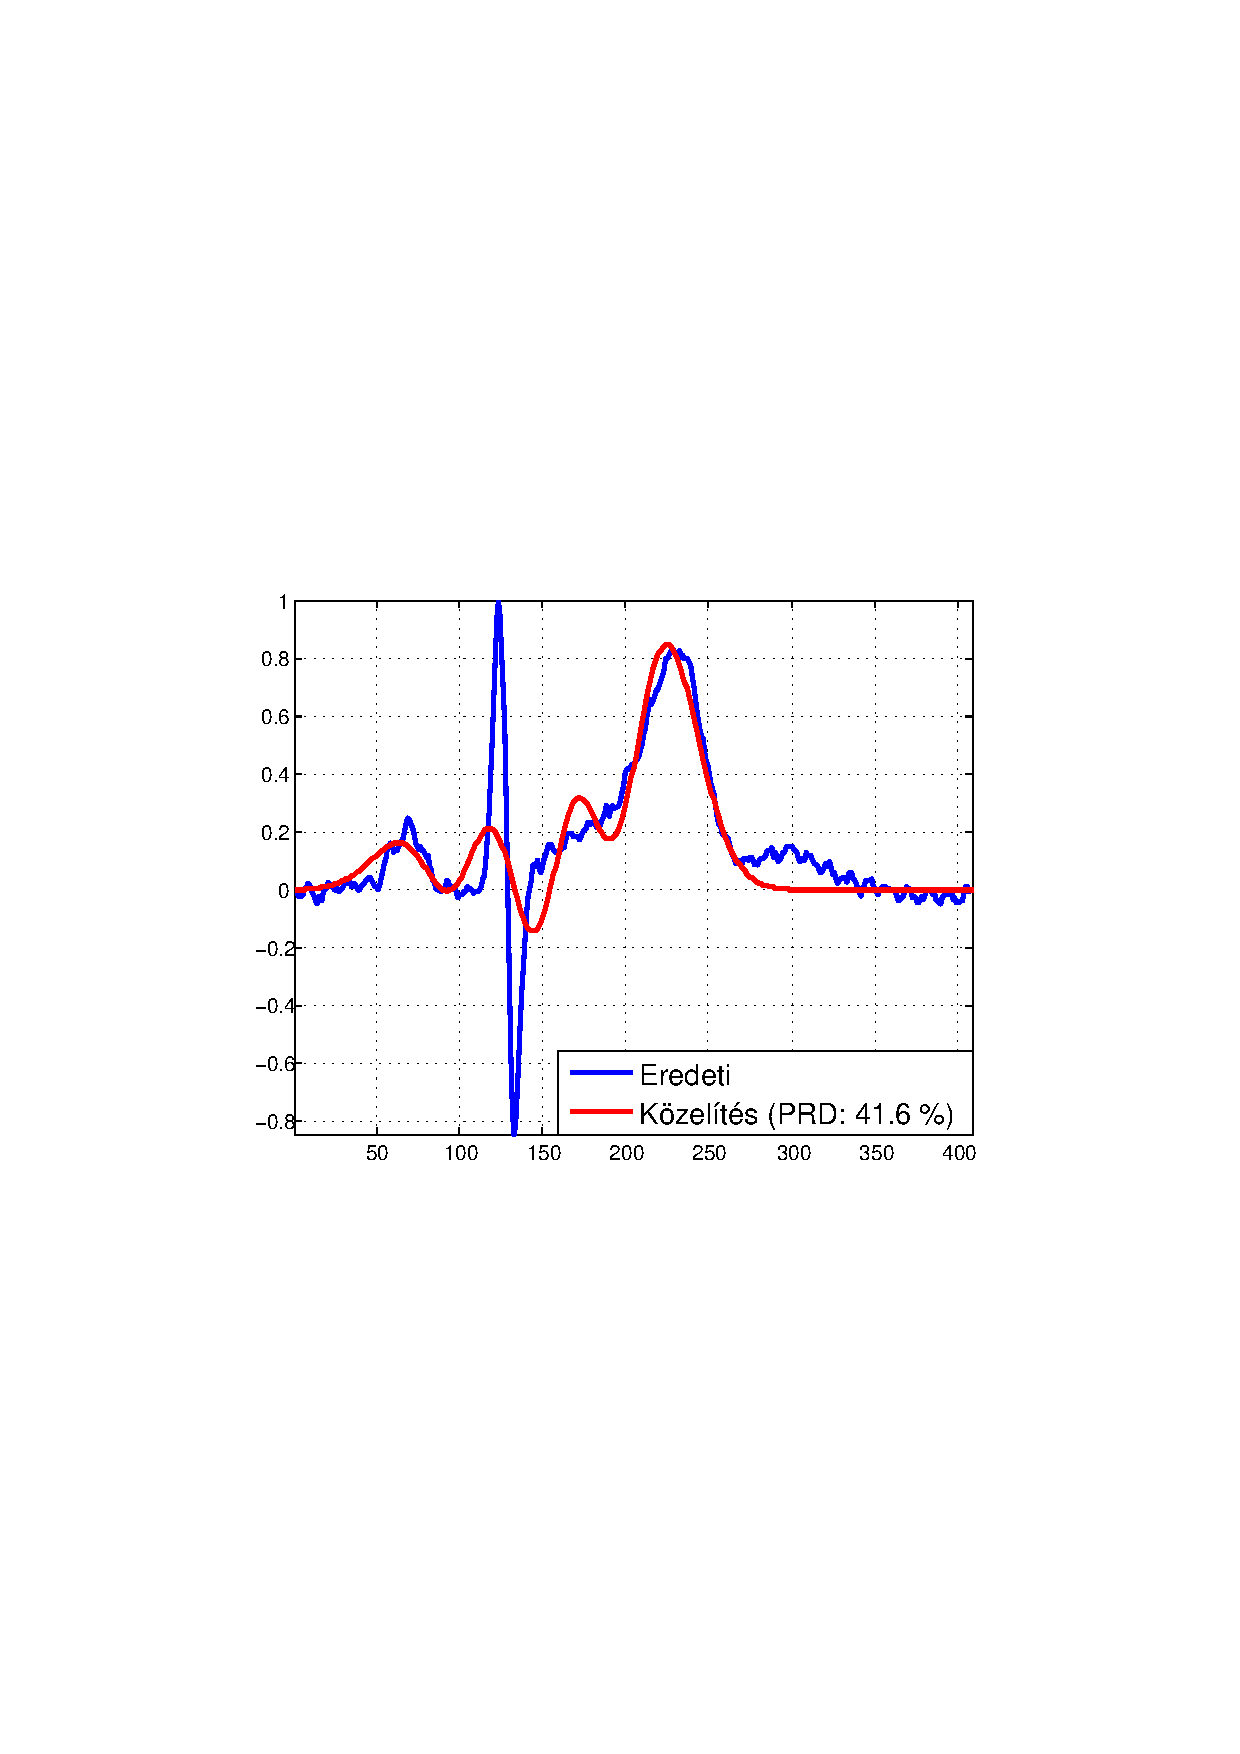
\includegraphics[scale=0.5,trim=100 280 100 280,clip]{./Abrak/Kitekintes/abra762_bad.pdf}}
\subfigure[Jó eset.]{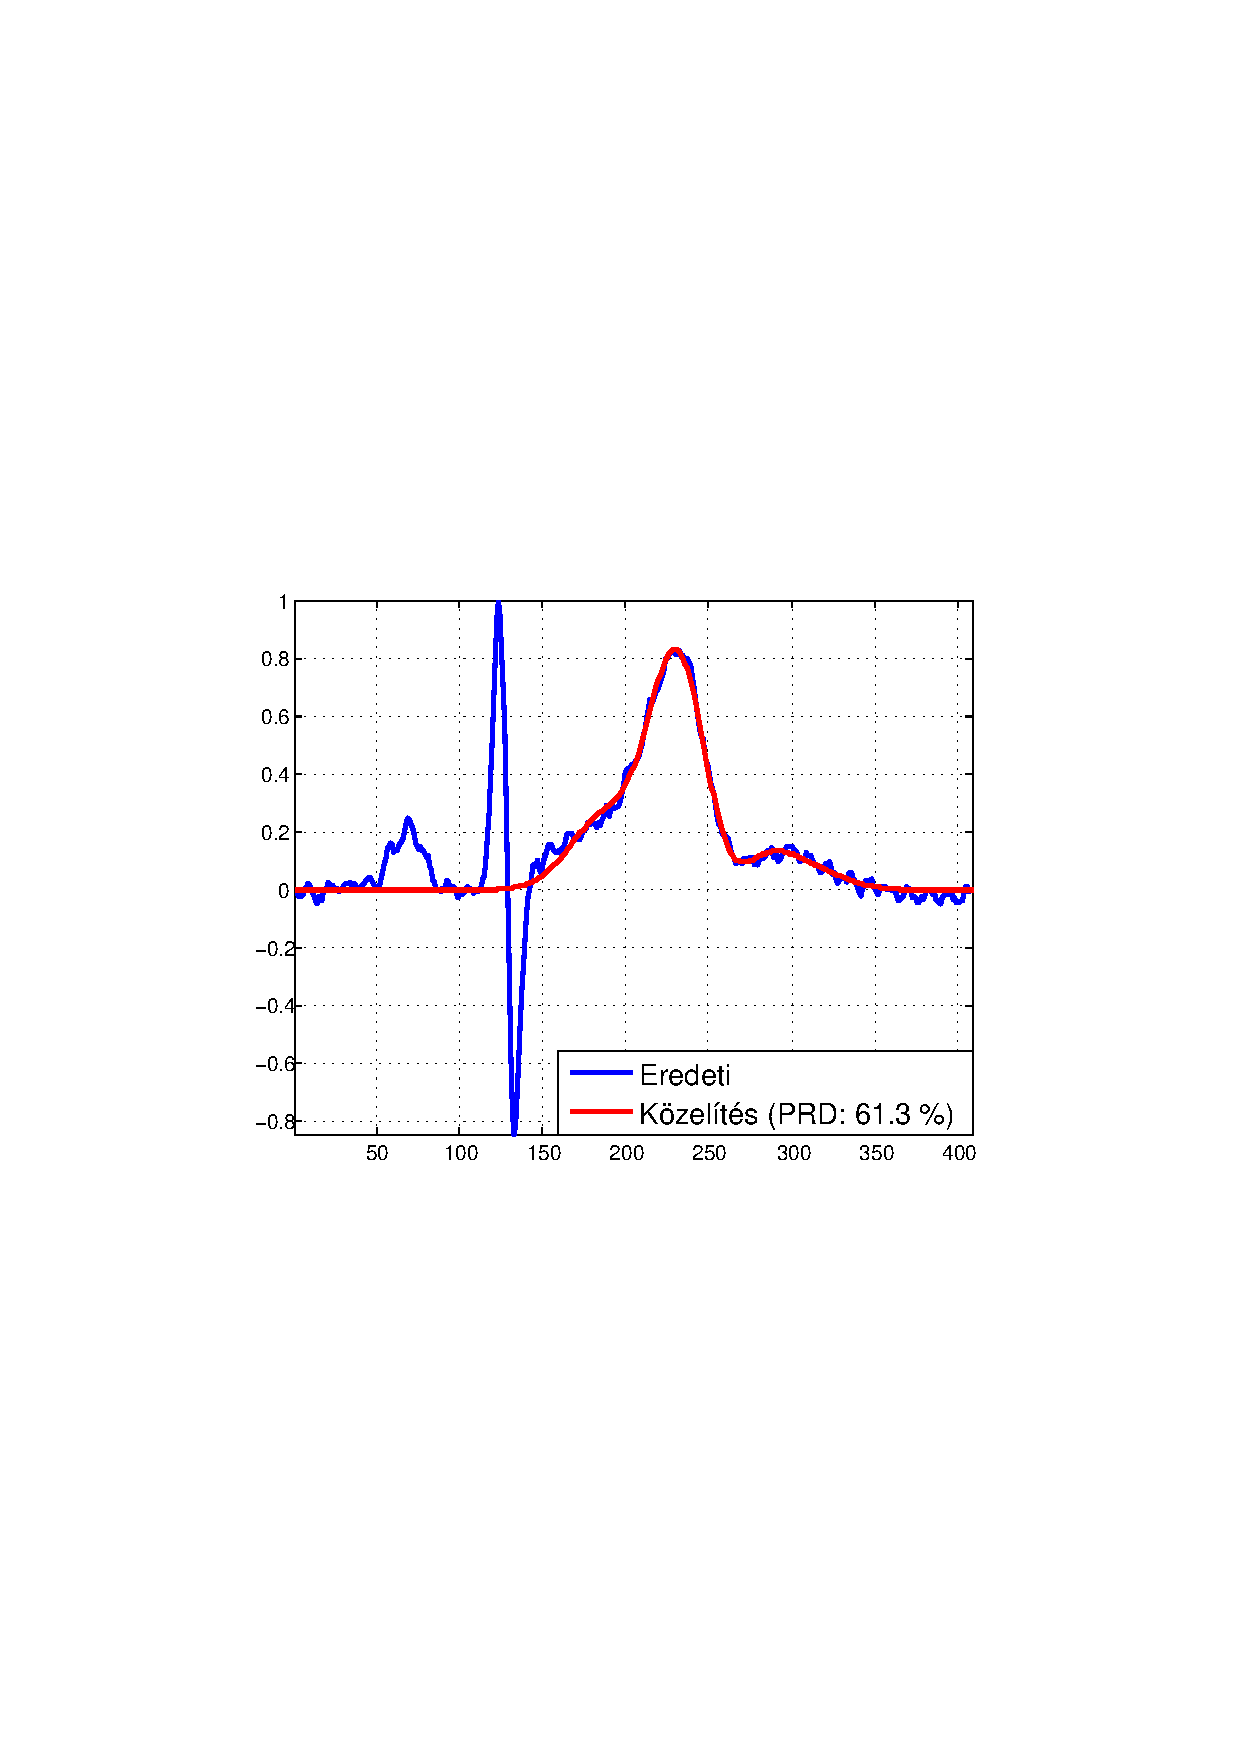
\includegraphics[scale=0.5,trim=100 280 100 280,clip]{./Abrak/Kitekintes/abra762_good.pdf}}
\caption{A mohó stratégia hátránya.}
\label{fig:counterexample}
\end{figure}	

\section{Eredmények a feladat specifikációjához képest}

A \ref{bevezetes:dolgozatspec} fejezetben bemutatásra került a feladat specifikációja, amely a dolgozatban bemutatott tömörítési eljárással, illetve az eljárás implementációjával kapcsolatban állított fel elvárásokat. A specifikáció első felében általános elvárások kerültek megfogalmazásra, melyek a tömörítő eljárást érintették. Ezek az elvárások röviden a következők: 

\begin{itemize}
\item A tömörítés kimenete egy olyan számsor legyen, amely pontosan reprezentálja a bemenetként kapott EKG felvételt, azonban álljon a bemenetnél kevesebb mintából.
\item A tömörítő eljárás szeparálja az egyes EKG felvételeken található szívütések szegmenseit. 
\item A tömörítő eljárás hatékonysága legyen összehasonlítható az idoralomban található egyéb eljárások hatékonyságával. 
\item A tömörítő eljárás szűrje az EKG felvételeken található zajt.
\end{itemize}

A \ref{eljaras tesztek} tesztek alapján elmondható, hogy a specifikációban megfogalmazott, tömörítő eljárással kapcsolatos elvárások közül mindegyik megvalósult. Az egyetlen kivételt a zajszűrés jelenti. A bemutatott algoritmus természetes módon szűri a bemenetkén kapott zajos felvételt, hiszen a mérést Hermite sima függvényekkel közelíti. A zajszűrés mértékének pontos meghatározása azonban további vizsgálatokat igényelne. 
\par A dolgozat elején bemutatott specifikáció második fele a tömörítő eljárás implementációjával szemben állít elvárásokat:

\begin{itemize}
\item Az implementációnak képesnek kell lennie az MIT-BIH adatbázisban található EKG felvételek tömörítésére. 
\item Az implementáció bemenetként a fennt említett adatbázisban található felvételt, illetve egy korábbi tömörítés következtében létrejött EKG reprezentációt kell elfogadnia.
\end{itemize} 

A \ref{modul tesztek} fejezetből látható, hogy az implementációval kapcsolatos legfontosabb elvárások közül mindegyiknek eleget tesz a tömörítő eljárás megvalósítása.  

\section{Köszönetnyilvánítás}



\chapter{Függelék}

A Függelék fejezet első része a felhasznát matematikai eszközök összefoglalását tartalmazza az \cite{szego, szoke} könyveket alapul véve. A matematikai eszközök bemutatásán kívül szintén ebben a fejezetben található a \ref{bevezetes transz dilat} fejezetben kimondott állítás bizonyítása. A Függelék fejezet végén a Nelder Mead optimalizációs algoritmus pszeudo kódja kerül ismertetésre. 

\section {Hermite  polinomok, Hermite függvények}
\subsubsection{Stirling  formula}
\begin{equation*}
n!\thicksim \sqrt {2\pi n}\Big(\frac ne\Big)^n,  \binom {2n} n\thicksim \frac {2^{2n}}{\sqrt{\pi n}}\ \ (
n\to\infty)
\end{equation*}

\subsubsection{\it  Rodrigues formula}
\begin{equation}
\begin{split}
&H_n(x):=e^{x^2}(-1)^n\left(\frac d{dx}\right)^n e^{-x^2}\ \ (n\in\Bbb N, x\in\Bbb R)\\
\end{split}
\end{equation}

\subsubsection{\it  Ortogonalitás, normált rendszer}
\begin{equation}
\begin{split}
&\int_{-\infty}^\infty e^{-x^2}H_n(x)H_m(x)\, dx=\pi^{1/2}2^n n!\, \delta_{mn}\ \ (m,n\in\Bbb N)\\
&\Phi_n(x):=H_n(x)e^{-x^2/2}/\sqrt{\pi^{1/2}2^n n!}=h_n(x)e^{-x^2/2} \ \ (n\in\Bbb N, x\in\Bbb R)\\
&\int_{-\infty}^\infty \Phi_n(x)\Phi_m(x)\, dx=\, \delta_{mn}\ \ (m,n\in\Bbb N)\\
&\int_{-\infty}^\infty e^{-x^2}\, dx=\pi^{1/2}<2
\end{split}
\end{equation}

\subsubsection{\it  Rekurziók}
\begin{equation}
\begin{split}
&H_n(x)=2xH_{n-1}(x)-2(n-1)H_{n-2}(x)\ (n\ge 2)\\
&H_{-1}(x)=0,  H_0(x)=1,\ \ H_1(x)=2x\\
&\Phi_n(x)=\sqrt{\frac 2 n}x\Phi_{n-1}-\sqrt{\frac {n-1} n}\Phi_{n-2}(x)\ (n\ge 2)\\ &\Phi_0(x)=e^{-x^2/2}/\pi^{1/4}, \Phi_1(x)= \sqrt 2 x e^{-x^2/2}/\pi^{1/4}\ \ (x\in\Bbb R)\\
&H'_n(x)=2nH_{n-1}(x)\ (n\in\Bbb N)\\
&\Phi'_n(x)=\sqrt{2n}\Phi_{n-1}(x)-x\Phi_n(x)\ \ (n\ge 0, x\in\Bbb R)\\
&\frac d{dx}(x\Phi_n(x))=(1-x^2)\Phi_n(x)+\sqrt{2n}x\Phi_{n-1}(x)\ \ (n\ge 1, x\in\Bbb R)
\label{eq:identities}
\end{split}
\end{equation}

\subsubsection{\it  Függvényértékek a $0$ helyen}
\begin{equation}
\begin{split}
&H_{2m+1}(0)=0,\ H_{2m}(0)=(-1)^m\frac{(2m)!}{m!}\\
&H'_{2m}(0)=0,\ H'_{2m+1}(0)=(-1)^m\frac{(2m+2)!}{(m+1)!}\\
&\Phi_{2m}(0)=(-1)^m2^{-m}\sqrt{\binom {2m}m}\thicksim (2 m)^{-1/4}\pi^{-1/2}\\
&\Phi'_{2m+1}(0)=(-1)^m2^{-m}\sqrt{\binom {2m}m}\thicksim (8m)^{1/4}\pi^{-1/2}
\end{split}
\end{equation}

\subsubsection{\it Kvadratúra formula}
$$
\int_{-\infty}^\infty e^{-x^2}f(x)\, dx\backsimeq \sum_{i=1}^n \lambda_{in}f(x_{in})
$$

$$
H_n(x_{in})=0,\ \lambda_{in}=\frac{\pi^{1/2}2^{n+1}n!}{[H'_n(x_{in}]^2}\ \ \  (n=1,2,\cdots, 1\le i\le n)
$$

\section{Approximáció afffin transzformáltakkal}
\label{app:aprx}

Jelölje a $\Bbb R$ számegyenesen szakaszonként folytonos, négyzetesen integrálható függvények terét $\mathcal F$. Az $\mathcal F$ téren jelentse
$$
\langle f,g\rangle:=\int_{-\infty}^\infty  f(x)g(x)\,dx
$$
a skaláris szorzatot.


\subsubsection{\it  Altértől vett távolság}

A  $\phi_n\in \mathcal F$ $(n\in\Bbb N)$ függvényrendszer  ortonormált, ha
$$
\langle \phi_n,\phi_m\rangle:=\delta_{mn}\ \ (m,n\in\Bbb N).
$$
Ebből a rendszerből az
$$
\ell(x)=\ell(x,\lambda, a)=\lambda x+a\ \ (x,a\in\Bbb R,\lambda>0)
$$
affin transzformációval származtatott
$$
\phi_n^{a,\lambda}(x):=\sqrt \lambda \phi_n(\lambda x+a)=\sqrt \lambda \phi_n(\ell(x)) \ (x,a\in\Bbb R,\lambda>0, n\in\Bbb N)
$$
rendszer szintén ortonormált. Valóban az $u=\ell(x)=\lambda x+a, dx=du/\lambda $ helyettesítéssel
\begin{equation}
\begin{split}
&\langle \phi_n^{a,\lambda},\phi_m^{a,\lambda}\rangle:=
\int_{-\infty}^\infty\lambda \phi_n(\lambda x+a)\phi_m(\lambda x+a)\, dx=\\
&=\int_{-\infty}^\infty \phi_n(u)\phi_m(u)\, dx=
\delta_{mn}\ \ (m,n\in\Bbb N).
\end{split}
\end{equation}
Jelölje  $X_n^{a,\lambda}$ a $\phi_0^{a,\lambda},\cdots,\phi_n^{a,\lambda}$ függvények által kifeszített alteret. Adott $f\in \mathcal F$ függvényhez a legközelebb eső $X_n^{a,\lambda}$-beli függvényt az
$$
S_n^{a,\lambda}f:=\sum_{k=0}^n \langle f,\phi_n^{a,\lambda}\rangle\phi_n^{a,\lambda}
$$
Fourier-projekcióval, az eltérés normájának a  négyzete  a
$$
D_n^2(a,\lambda):=\|f-S_n^{a,\lambda}f\|^2=\langle f,f\rangle-\sum_{k=0}^n |\langle f,\phi_k^{a,\lambda}\rangle|^2
$$
függvénnyel adható meg. A $D_n(a,\lambda)$ minimumának meghatározása ekvivalens az
$$
F_n(a,\lambda):=\sum_{k=0}^n |\langle f,\phi_k^{a,\lambda}\rangle|^2\ \
((a,\lambda)\in T:=\{(p,q)\in\Bbb R^2:p\in\Bbb R, q>0\}
$$
függvény maximumának meghatározásával.

\subsubsection{\it  Becslések az $F_n$ függvényre}

 A továbbiakban a
 $$
 \phi_n(x)=\Phi_n(x)=h_n(x)e^{-x^2/2}\ \ (x\in\Bbb R, n\in\Bbb N)
 $$
 normált Hermite-függvényeket választjuk ortonormált rendszernek. Ekkor
 \begin{equation}
 \begin{split}
 &|\Phi_n(x)|\le M_n e^{-x^2/4}\le M_n, \ |\Phi_n'(x)|\le N_n e^{-x^2/4}\le N_n\ (x\in\Bbb R, n\in\Bbb N)\\
 &M_n:=\max_{x\in\Bbb R}|h_n(x)|e^{-x^2/4},\ N_n:=\max_{x\in\Bbb R}|h'_n(x)-xh_n(x)|e^{-x^2/4}\\
 &\int_{-\infty}^\infty|\Phi_n(x)|\, dx\le M_n\int_{-\infty}^\infty e^{-x^2/4}\, dx<4M_n
 \end{split}
 \end{equation}
 Ezeket felhasználva becsléseket adhatóak az
 $$
 A_k(a,\lambda):=\langle f,\phi_k^{a,\lambda}\rangle=\sqrt{\lambda}\int_{-\infty}^\infty f(x)\phi_k(\lambda x+a)\, dx=\frac 1{\sqrt{\lambda}}\int_{-\infty}^\infty f((u-a)/\lambda)\phi_k(u)\, du
 $$
 Fourier-együtthatókra. A továbbiakban kompakt tartójú, korlátos függvényekből indulunk ki. Nem jelenti az általánosság megszorítását a következő feltételezés:
 $$
 f(x)=0,\ \text{ha}\ |x|\ge 1,\ \ |f(x)|\le 1 \ (x\in\Bbb R).
 $$
 A paraméteres integrálokra vonatkozó tételből  következik, hogy   az
 $$
 F_n(a,\lambda):=\sum_{k=0}^n|A_k(a,\lambda)|^2\ \ \  ((a,\lambda)\in T>0)
 $$
 függvény folytonosan  differenciálható. A következőkben bemutatásra kerül, hogy az $F_n:T\to [0,\infty)$
 folytonos függvénynek van maximuma a $T$ (nem kompakt) halmazon.

 A fenti egyenlőtlenségekből következik, hogy
 \begin{equation}
 \begin{split}
 &|A_k(\lambda,a)|\le \sqrt{\lambda} M_k\int_{-\infty}^\infty |f(x)|\, dx\le 2M_k\sqrt{\lambda}\ \ (\lambda\le 1)\\
 &|A_k(\lambda,a)|\le\frac 1{\sqrt{\lambda}}\int_{-\infty}^\infty |\Phi_k(u)|\, du\le
 \frac {4M_k}{\sqrt{\lambda}}\ (\lambda\ge 1),
 \end{split}
 \end{equation}
 továbbá $\lambda\ge 1,\ a\ge 2\lambda $ eset\'en
 \begin{equation}
 \begin{split}
 &|A_k(\lambda,a)|\le \frac 1{\sqrt{\lambda}}\int_{a-\lambda}^{a+\lambda}|\Phi_k(u)|\, du
 \le \frac 1{\sqrt{\lambda}}\int_{a-\lambda}^\infty |\Phi_k(u)|\, du\le\\
 &\le \frac {M_k}{\sqrt{\lambda}}\int_\lambda^\infty e^{-{u^2}/4}\, du<
 \frac {M_k}{\sqrt{\lambda}}\int_\lambda^\infty u e^{-{u^2}/4}\, du=
 2 M_k\sqrt{\lambda} e^{-{\lambda^2}/4}<\frac {8M_k}{\sqrt{\lambda}}
\end{split}
\end{equation}
Hasonlóan egyenlőtlenséget ad az $a<-2\lambda$ eset. Innen következik, hogy az
$$
T_s:=\{(p,q): -2s\le p\le 2s, 1/s\leq p \le s\}
$$
téglalapon kívül  érvényes a
$$
\sup_{(a,\lambda) \notin T_s}|A_k(a,\lambda)|\le \frac {8M_k}{\sqrt s}\ \  (s>1)
$$
becslés. Ennek alapján nyilvánvaló, hogy az $F_n$  függvénynek létezik a maximuma a $T$ téglelapon.

\iffalse
Célunk az
 maximum meghat\'aroz\'asa a leggyorsabb ereszked\'es elve alapj\'an. Bevezetve az $s(u)=\ell^{-1}(u)=(u-a)/\lambda$ jel\"ol\'est, a  param\'eteres integr\'al differenci\'al\'asi szab\'alya alapj\'an  azt kapjuk, hogy
\begin{equation}
\begin{split}
&\frac \partial {\partial a}A_k(a,\lambda)=\lambda^{1/2} \int_{-\infty}^\infty f(x)\phi_k'(\ell(x))\, dx\\
 &\frac \partial {\partial \lambda}A_k(a,\lambda)=\lambda^{1/2} \int_{-\infty}^\infty f(x)x\phi_k'(\ell(x))\, dx+\frac 12\lambda^{-1/2}\int_{-\infty}^\infty f(x)\phi_k(\ell(x))
 \end{split}
 \end{equation}



 A parci\'alis deriv\'altak a k\"ovetkez\H o h\'arom sorozattal fejezehet\H ok ki:
 \begin{equation}
 \begin{split}
 &A_k(a,\lambda):=\sqrt{\lambda}\int_{-\infty}^\infty f(x)\phi_k(\ell(x))\, dx\\
 &A_k^{[1]}(a,\lambda):=\sqrt{\lambda}\int_{-\infty}^\infty f(x))\phi_k'(\ell(x))\, dx\\
 &A_k^{[2]}(a,\lambda):=\sqrt{\lambda}\int_{-\infty}^\infty xf(x))\phi_k'(\ell(x))\, dx.
 \end{split}
  \end{equation}
Nevezetesen
\begin{equation}
\begin{split}
&F(a,\lambda)=\sum_{k=0}^n A_k^2(a,\lambda)\\
&\frac 12\frac \partial{\partial a} F(\lambda, a)=\sum_{k=0}^n A_k(a,\lambda)A_k^{[1]}(a,\lambda)\\
&\frac 12\frac \partial{\partial \lambda} F(a,\lambda)=\frac 1{2\lambda}\sum_{k=0}^n A_k^2(a,\lambda)+\sum_{k=0}^n A_k(\lambda,a)A_k^{[2]}(a,\lambda)=\\
&=\frac 1{2\lambda} F(a,\lambda )+\sum_{k=0}^n A_k(\lambda,a)A_k^{[2]}(\lambda,a)
\end{split}
\end{equation}

\fi

\section{Algoritmusok}


\iffalse

%\section{PSO pszeudok\'od}
\begin{algorithm}[htp] 
\begin{algorithmic}[1]
	\Function{PSO}{$Hiba,\,S,\,I_N,c_{1,2}$} 		
	\ForAll{$k\gets 1, S$} %\Comment{In our case, $c_1=1.5,\,c_2=2$ and $V_{max}=0.5\,.$}
		\State Randomize $\lambda_k,\; a_k, \; v_k$	 		
		\State Initialize $H_k.\lambda:=\lambda_k$ \Comment{A r\'eszecsk\'ehez tartoz\'o dilat\'aci\'o}
		\State Initialize $H_k.a:=a_k$		\Comment{A r\'eszecsk\'ehez tartoz\'o transzl\'aci\'o}	
		\State Initialize $H_k.pBest:=[\lambda_k, a_k]$    \Comment{A r\'eszecske legjobb poz\'\i ci\'oja}
		\State Initialize $H_k.pDBest:=\infty$   \Comment{A r\'eszecske legkisebb hib\'aja}
		\State Initialize $H_k.v:=v_k$   \Comment{A r\'eszecske kezd\H o gyorsul\'asa}
	\EndFor
	\For{$\ell\gets 1, I_N$}	
		\For{$k\gets 1, S$}								
			\If{$Hiba(H_k)<H_k.pDBest$}  \Comment{pBest friss\'\i t\'ese}
				\State $H_k.pBest=[\lambda_k, a_k]$
				\State $H_k.pDBest= Hiba(H_k)$
			\EndIf
		\EndFor		
		\If{$Hiba(H_k)<\underset{1\leq k\leq S}{\min}\, Hiba(H_k)$}  \Comment{gBest friss\'\i t\'ese}
				\State $gBest=[H_k.\lambda, H_k.a]$
			\EndIf

	\For{$k\gets 1, S$}						\Comment{gyorsul\'as \'es poz\'\i ci\'o friss\'\i t\'ese}
			\State $H_k.v = H_k.v + c_1 r_1 \cdot (H_k.pBest-[\lambda_k, a_k]) 
						 + c_2 r_2 \cdot (gBest-[\lambda_k, a_k])$ 
			\State $H_k.\lambda = H_k.\lambda + H_k.v$	
			\State $H_k.a = H_k.a + H_k.v$
			
		\EndFor					
	\EndFor
	\State \textbf{return} $gBest$
	\EndFunction
\end{algorithmic}
\caption{Particle Swarm Optimization}
\label{alg:pso}
\end{algorithm}

\fi

\newpage
%\section{Nelder-Mead pszeudok\'od}
Az indexek rendezésénél
$y_3\le y_2\le y_1$ teljesül. Az $IterLepes(5)$ rutin az 
$(x_1,x_2,x_3)$ hármast a $T_5$ transzformációval kapott
hármasra cseréli.
\bigskip

\begin{algorithm}[htb!] 
\begin{algorithmic}[1]
	\Function{Nelder-Mead}{} 
	\If{$y_3 \leq y_4 \wedge y_4 < y_2$}
		\State $x_1 = x_4$
	\ElsIf{$y_4 < y_3$}
		\If{$y_5 < y_4$}
			\State $x_1 = x_5$
		\Else
			\State $x_1 = x_4$
		\EndIf
	\ElsIf{$y_4 \geq y_2$}
		\If{$y_4 < y_1$}
			\If{$y_6 \leq y_4$}
				\State $x_1 = x_6$
			\Else
				\State $IterLepes(5)$
			\EndIf
		\ElsIf{$y_4 \geq y_1$}
			\If{$y_7 < y_3$}
				\State $x_1 = x_7$
			\Else
				\State $IterLepes(5)$
			\EndIf
		\EndIf
	\EndIf
	\EndFunction
\end{algorithmic}
\caption{Nelder-Mead}
\label{alg:NM}
\end{algorithm}

\end{document}
